% Options for packages loaded elsewhere
% Options for packages loaded elsewhere
\PassOptionsToPackage{unicode}{hyperref}
\PassOptionsToPackage{hyphens}{url}
\PassOptionsToPackage{space}{xeCJK}
%
\documentclass[
  12pt,
  letterpaper,
]{scrreprt}
\usepackage{xcolor}
\usepackage[left=1in,right=1in,top=1in,bottom=1in]{geometry}
\usepackage{amsmath,amssymb}
\setcounter{secnumdepth}{2}
\usepackage{iftex}
\ifPDFTeX
  \usepackage[T1]{fontenc}
  \usepackage[utf8]{inputenc}
  \usepackage{textcomp} % provide euro and other symbols
\else % if luatex or xetex
  \usepackage{unicode-math} % this also loads fontspec
  \defaultfontfeatures{Scale=MatchLowercase}
  \defaultfontfeatures[\rmfamily]{Ligatures=TeX,Scale=1}
\fi
\usepackage{lmodern}
\ifPDFTeX\else
  % xetex/luatex font selection
  \setmainfont[]{Crimson}
  \ifXeTeX
    \usepackage{xeCJK}
    \setCJKmainfont[]{Noto Serif KR}
  \fi
  \ifLuaTeX
    \usepackage[]{luatexja-fontspec}
    \setmainjfont[]{Noto Serif KR}
  \fi
\fi
% Use upquote if available, for straight quotes in verbatim environments
\IfFileExists{upquote.sty}{\usepackage{upquote}}{}
\IfFileExists{microtype.sty}{% use microtype if available
  \usepackage[]{microtype}
  \UseMicrotypeSet[protrusion]{basicmath} % disable protrusion for tt fonts
}{}
\makeatletter
\@ifundefined{KOMAClassName}{% if non-KOMA class
  \IfFileExists{parskip.sty}{%
    \usepackage{parskip}
  }{% else
    \setlength{\parindent}{0pt}
    \setlength{\parskip}{6pt plus 2pt minus 1pt}}
}{% if KOMA class
  \KOMAoptions{parskip=half}}
\makeatother
% Make \paragraph and \subparagraph free-standing
\makeatletter
\ifx\paragraph\undefined\else
  \let\oldparagraph\paragraph
  \renewcommand{\paragraph}{
    \@ifstar
      \xxxParagraphStar
      \xxxParagraphNoStar
  }
  \newcommand{\xxxParagraphStar}[1]{\oldparagraph*{#1}\mbox{}}
  \newcommand{\xxxParagraphNoStar}[1]{\oldparagraph{#1}\mbox{}}
\fi
\ifx\subparagraph\undefined\else
  \let\oldsubparagraph\subparagraph
  \renewcommand{\subparagraph}{
    \@ifstar
      \xxxSubParagraphStar
      \xxxSubParagraphNoStar
  }
  \newcommand{\xxxSubParagraphStar}[1]{\oldsubparagraph*{#1}\mbox{}}
  \newcommand{\xxxSubParagraphNoStar}[1]{\oldsubparagraph{#1}\mbox{}}
\fi
\makeatother


\usepackage{longtable,booktabs,array}
\usepackage{calc} % for calculating minipage widths
% Correct order of tables after \paragraph or \subparagraph
\usepackage{etoolbox}
\makeatletter
\patchcmd\longtable{\par}{\if@noskipsec\mbox{}\fi\par}{}{}
\makeatother
% Allow footnotes in longtable head/foot
\IfFileExists{footnotehyper.sty}{\usepackage{footnotehyper}}{\usepackage{footnote}}
\makesavenoteenv{longtable}
\usepackage{graphicx}
\makeatletter
\newsavebox\pandoc@box
\newcommand*\pandocbounded[1]{% scales image to fit in text height/width
  \sbox\pandoc@box{#1}%
  \Gscale@div\@tempa{\textheight}{\dimexpr\ht\pandoc@box+\dp\pandoc@box\relax}%
  \Gscale@div\@tempb{\linewidth}{\wd\pandoc@box}%
  \ifdim\@tempb\p@<\@tempa\p@\let\@tempa\@tempb\fi% select the smaller of both
  \ifdim\@tempa\p@<\p@\scalebox{\@tempa}{\usebox\pandoc@box}%
  \else\usebox{\pandoc@box}%
  \fi%
}
% Set default figure placement to htbp
\def\fps@figure{htbp}
\makeatother


% definitions for citeproc citations
\NewDocumentCommand\citeproctext{}{}
\NewDocumentCommand\citeproc{mm}{%
  \begingroup\def\citeproctext{#2}\cite{#1}\endgroup}
\makeatletter
 % allow citations to break across lines
 \let\@cite@ofmt\@firstofone
 % avoid brackets around text for \cite:
 \def\@biblabel#1{}
 \def\@cite#1#2{{#1\if@tempswa , #2\fi}}
\makeatother
\newlength{\cslhangindent}
\setlength{\cslhangindent}{1.5em}
\newlength{\csllabelwidth}
\setlength{\csllabelwidth}{3em}
\newenvironment{CSLReferences}[2] % #1 hanging-indent, #2 entry-spacing
 {\begin{list}{}{%
  \setlength{\itemindent}{0pt}
  \setlength{\leftmargin}{0pt}
  \setlength{\parsep}{0pt}
  % turn on hanging indent if param 1 is 1
  \ifodd #1
   \setlength{\leftmargin}{\cslhangindent}
   \setlength{\itemindent}{-1\cslhangindent}
  \fi
  % set entry spacing
  \setlength{\itemsep}{#2\baselineskip}}}
 {\end{list}}
\usepackage{calc}
\newcommand{\CSLBlock}[1]{\hfill\break\parbox[t]{\linewidth}{\strut\ignorespaces#1\strut}}
\newcommand{\CSLLeftMargin}[1]{\parbox[t]{\csllabelwidth}{\strut#1\strut}}
\newcommand{\CSLRightInline}[1]{\parbox[t]{\linewidth - \csllabelwidth}{\strut#1\strut}}
\newcommand{\CSLIndent}[1]{\hspace{\cslhangindent}#1}



\setlength{\emergencystretch}{3em} % prevent overfull lines

\providecommand{\tightlist}{%
  \setlength{\itemsep}{0pt}\setlength{\parskip}{0pt}}



 


\addtokomafont{disposition}{\rmfamily}
\KOMAoptions{chapterprefix=true,appendixprefix=true}
\KOMAoptions{headings=small}
\setkomafont{pageheadfoot}{\normalfont\normalcolor\footnotesize}
\setkomafont{pagenumber}{\normalfont\normalcolor\footnotesize}
\usepackage{tocbibind}  % Include TOC, List of Figures, and List of Tables in the TOC
\usepackage{fontspec}    % Ensure font support
\usepackage{placeins}
\usepackage{float}
\usepackage{setspace}
\usepackage{indentfirst}
\usepackage{chngcntr}
\counterwithin{figure}{subsection}
\usepackage{gb4e} \noautomath
\usepackage{booktabs}
\usepackage{longtable}
\usepackage{array}
\usepackage{multirow}
\usepackage{wrapfig}
\usepackage{float}
\usepackage{colortbl}
\usepackage{pdflscape}
\usepackage{tabu}
\usepackage{threeparttable}
\usepackage{threeparttablex}
\usepackage[normalem]{ulem}
\usepackage{makecell}
\usepackage{xcolor}
\makeatletter
\@ifpackageloaded{bookmark}{}{\usepackage{bookmark}}
\makeatother
\makeatletter
\@ifpackageloaded{caption}{}{\usepackage{caption}}
\AtBeginDocument{%
\ifdefined\contentsname
  \renewcommand*\contentsname{Table of contents}
\else
  \newcommand\contentsname{Table of contents}
\fi
\ifdefined\listfigurename
  \renewcommand*\listfigurename{List of Figures}
\else
  \newcommand\listfigurename{List of Figures}
\fi
\ifdefined\listtablename
  \renewcommand*\listtablename{List of Tables}
\else
  \newcommand\listtablename{List of Tables}
\fi
\ifdefined\figurename
  \renewcommand*\figurename{Figure}
\else
  \newcommand\figurename{Figure}
\fi
\ifdefined\tablename
  \renewcommand*\tablename{Table}
\else
  \newcommand\tablename{Table}
\fi
}
\@ifpackageloaded{float}{}{\usepackage{float}}
\floatstyle{ruled}
\@ifundefined{c@chapter}{\newfloat{codelisting}{h}{lop}}{\newfloat{codelisting}{h}{lop}[chapter]}
\floatname{codelisting}{Listing}
\newcommand*\listoflistings{\listof{codelisting}{List of Listings}}
\makeatother
\makeatletter
\makeatother
\makeatletter
\@ifpackageloaded{caption}{}{\usepackage{caption}}
\@ifpackageloaded{subcaption}{}{\usepackage{subcaption}}
\makeatother
\usepackage{bookmark}
\IfFileExists{xurl.sty}{\usepackage{xurl}}{} % add URL line breaks if available
\urlstyle{same}
\hypersetup{
  pdftitle={Multi-Word Representations in Minds and Models},
  pdfauthor={Zachary Nicholas Houghton},
  hidelinks,
  pdfcreator={LaTeX via pandoc}}


\title{Multi-Word Representations in Minds and Models}
\usepackage{etoolbox}
\makeatletter
\providecommand{\subtitle}[1]{% add subtitle to \maketitle
  \apptocmd{\@title}{\par {\large #1 \par}}{}{}
}
\makeatother
\subtitle{Investigating the Storage of Multi-Word Phrases in Humans and
Large Language Models}
\author{Zachary Nicholas Houghton}
\date{}
\begin{document}
\pagenumbering{roman}
\cleardoublepage
\thispagestyle{plain}
\begin{center}
   \null\vfill
   \textbf{%
      Multi-Word Representations in Minds and Models:\\
	  Investigating the Storage of Multi-Word Phrases in Humans and Large
  Language Models
   }%
   \\
   \bigskip
   By \\
   \bigskip
   {Zachary Nicholas Houghton}
\\   
   %2020 EDIT: Removed double-spacing btwn name and DISSERTATION   
   %\bigskip
   %B.S. (University of California, Davis) 2001 \\
   %\bigskip
   %2019 EDIT: Removed line for previous degree.
   DISSERTATION \\
   \bigskip
   Submitted in partial satisfaction of the requirements for the
   degree of \\
   \bigskip
   DOCTOR OF PHILOSOPHY \\
   \bigskip
   in \\
   \bigskip
   {Linguistics} \\ 
      \bigskip
   in the \\
   \bigskip
   OFFICE OF GRADUATE STUDIES \\
   \bigskip        
   of the \\
   \bigskip
   UNIVERSITY OF CALIFORNIA \\
   \bigskip
   DAVIS \\
   \bigskip
   Approved: \\
   \bigskip
   \bigskip
   \makebox[3in]{\hrulefill} \\
   Dr.~Emily Morgan, Chair \\
   \bigskip
   \bigskip
   \makebox[3in]{\hrulefill} \\
   Dr.~Masoud Jasbi \\
   \bigskip
   \bigskip
   \makebox[3in]{\hrulefill} \\
   Dr.~Fernanda Ferreira \\
   \bigskip
   Committee in Charge \\
   \bigskip
   2024 \\
   \vfill
\end{center}


\newpage
\newcounter{savedpage}
\setcounter{savedpage}{\value{page}}

\thispagestyle{empty}
\begin{titlepage}
\vspace*{\stretch{1}}
\begin{center}
  Copyright \copyright\ 2025 by Zachary Nicholas Houghton. \\
  \textit{All rights reserved.}
\end{center}
\end{titlepage}

\setcounter{page}{\value{savedpage}} % Reset the counter
\clearpage
\renewcommand*\contentsname{Table of contents}
{
\setcounter{tocdepth}{2}
\tableofcontents
}
\listoffigures
\listoftables

\bookmarksetup{startatroot}

\chapter*{Abstract}\label{sec-abstract}
\addcontentsline{toc}{chapter}{Abstract}

\markboth{Abstract}{Abstract}

This is my abstract.

\newpage

\bookmarksetup{startatroot}

\chapter*{Acknowledgements}\label{sec-acknowledgements}
\addcontentsline{toc}{chapter}{Acknowledgements}

\markboth{Acknowledgements}{Acknowledgements}

First and foremost, I would not be here if it weren't for my advisor,
Dr.~Emily Morgan. Emily has been a never-ending source of knowledge and
a constant source of reassurance. Emily was charged with the non-trivial
task of helping to translate my incoherent stream of thoughts into a
coherent set of ideas. She pushed me hard, believed in me, and never let
me fall behind. I'm extraordinarily fortunate to have had her as my
advisor.

I'd also like to thank many of the other professors here who have been
crucial to my development as a linguist. Specifically, I'd like to thank
Dr.~Fernanda Ferreira whose knowledge of the field is so expansive that
she can, without delay, provide a reference for any psycholinguistic
phenomenon one can think of. I'd also like Dr.~Kenji Sagae for his help
over the years regarding all things natural language processing.
Additionally, I'd like to thank Dr.~Santiago Barreda who has provided a
great deal of advice and help with statistical analyses. Finally, I'd
like to thank Dr.~Masoud Jasbi who has taught me the importance of
various linguistics theories, even those I don't agree with.

Many of the ideas presented here have benefited in some form or another
from feedback from many brilliant graduate students. I would especially
like to thank Dingyi (Penny) Pan and Casey Felton for their feedback on
much of the work included here.

I'd also like to thank Casey, Felix, and Nora for being a strong support
system during my time here. Our Sunday shenanigans were a welcomed
escape from the tireless work of completing a PhD.

My journey in linguistics started at the University of Oregon, and I
want to thank all of the professors that supported the beginning of my
journey. I particularly want to acknowledge Dr.~Vsevolod Kapatsinski.
Volya has donated countless hours of his time to me even after his role
as my undergraduate thesis advisor was long over. He continues to be an
endless source of knowledge and inspiration and much of my knowledge and
interest in language learning comes from him. Perhaps more importantly,
however, he is a constant reminder that linguistics is \emph{fun}! Had
it not been for our meetings over the years that devolved into
ridiculous linguistic tangents, I would have burnt out long ago.

I would also like to thank Kim 선생님 who encouraged me to apply for
graduate school in the first place and believed in me often times more
than I believed in myself.

In addition, I want to thank Dr.~Melissa Baese-Berk and Dr.~Misaki Kato,
and Dr.~Zara Harmon. A great deal of my success as a graduate student
came from their mentorship.

Along with the technical and academic guidance, it also would have been
impossible to complete this PhD without the unending support I received
from so many people in my personal life.

Specifically, I have been fortunate to have a strong support system in
the form of of my two sisters, Kayla and Lily. We've been through so
much together. I don't know where I would be, not just academically, but
more generally in life, had you two not been by my side.

This work would also have not been completed without the influence of my
parents. Specifically, I want to thank my mom for teaching me that the
ability to find the answer is far more important than knowing the
answer, and my dad, for teaching me the discipline and practical skills
to achieve my goals.

For both my undergraduate and graduate studies, I made the difficult
decision to pursue my education on the opposite side of the country from
my hometown in Connecticut. Despite the physical distance, I have always
been able to count on my friends back east---not only during the easier
times, but, more importantly, through the more challenging ones. Addy,
Charles, Paul, Spencer, Wyatt, and 보미: thank you for being such a
strong and constant support network.

Finally, to all the people I met during these five years at UC Davis:
you welcomed me and gave me a home. You supported me, believed in me,
and pushed me to be the best version of myself. I'm exceptionally proud
to be an Aggie.

The number of people who have been indispensable in me getting here is
undoubtedly larger than is feasible to include here. To those that I
have inevitably left out, I apologize.

\bookmarksetup{startatroot}

\chapter{Introduction}\label{introduction}

\pagenumbering{arabic}

\doublespacing

\setlength{\parindent}{4em}

How much of language is memorized and how much is improvised? Every time
we speak, we are faced with the choice between familiar expressions,
like \emph{I don't know}, and novel constructions, like \emph{to me it
is uncertain}. In other words, we constantly navigate a trade-off
between stored, item-specific knowledge -- our stored knowledge of
particular words and phrases -- and abstract knowledge, which allows us
to combine those stored representations in new ways.

From a young age, humans are capable of generating sentences that we've
never encountered before
(\citeproc{ref-berkoChildsLearningEnglish1958}{Berko, 1958}). This
ability is largely enabled by an ability to store forms (storage) that
we've learned and combine them (computation) into new forms using our
knowledge of the grammar
(\citeproc{ref-berkoChildsLearningEnglish1958}{Berko, 1958};
\citeproc{ref-morganModelingIdiosyncraticPreferences2015}{Morgan \&
Levy, 2015a}, \citeproc{ref-morganAbstractKnowledgeDirect2016}{2016a},
\citeproc{ref-morgan2024}{2024};
\citeproc{ref-stembergerFrequencyLexicalStorage1986}{Stemberger \&
MacWhinney, 1986},
\citeproc{ref-stembergerAreInflectedForms2004}{2004}). In theory,
storage and computation can be complementary forces: if a form is
stored, it does not necessarily need to be computed, and if a meaning
can be generated via computation, it does not necessarily need to be
stored. For example, if the word \emph{cats} is stored, then it is not
necessary to compute it (e.g., by combining the lexical root,
\emph{cat}, with a general plural rule, -\emph{s}). On the other hand,
if it can be computed (e.g., if we have learned the word \emph{cat} and
we have learned how to make regular forms plural in English), then we do
not necessarily need to store it. However, the fact that computation and
storage can be independent does not preclude the possibility of items
being both stored holistically and able to be formed compositionally.
Indeed, a surge of research in the last few decades has suggested the
opposite: that a rich amount of language, including words and multi-word
phrases, is stored holistically (e.g., \citeproc{ref-bybee2003}{Bybee,
2003}; \citeproc{ref-morgan2015}{Morgan \& Levy, 2015b},
\citeproc{ref-morganAbstractKnowledgeDirect2016}{2016a},
\citeproc{ref-morgan2024}{2024};
\citeproc{ref-stembergerFrequencyLexicalStorage1986}{Stemberger \&
MacWhinney, 1986},
\citeproc{ref-stembergerAreInflectedForms2004}{2004}).

The evidence that more complex forms, such as multi-morphemic words and
phrases, may be stored holistically begs a host of questions. For
example, what factors determine whether a phrase is stored holistically
or generated compositionally using knowledge of the grammar? If
\emph{pick up} is stored holistically, then under what circumstances
does a listener use their knowledge of the grammar to form the phrase
compositionally and under what circumstances do they access the
holistically stored representation? Similarly, how do compositional
forms interact with their holistically stored counterparts during
processing? When listeners hear \emph{pick}, are they able to activate
the representation of the holistically stored form \emph{pick up} before
hearing \emph{up}? Finally, how do stored representations differ from
the individual word-level representations? Is the representation of
\emph{pick up} completely disconnected from the individual
representations of \emph{pick} and \emph{up}, despite the fact that they
have overlapping acoustics (i.e., when hearing \emph{pick up} one
necessarily hears \emph{pick} and \emph{up})?

The present section introduces the relevant background for each of these
questions. Section~\ref{sec-accounts-of-storage} describes the current
debates about storage.
Section~\ref{sec-evidence-of-storage-in-words-and-phrases} explores the
evidence for the holistic storage of multi-morphemic words and
multi-word phrases. Section~\ref{sec-factors-that-drive-storage} reviews
the evidence for factors that drive storage.
Section~\ref{sec-representations-of-stored-items} examines how stored
items are represented.
Section~\ref{sec-processing-consequences-of-storage} examines the
processing consequences of holistic storage.
Section~\ref{sec-storage-in-humans-vs-large-language-models} examines
how large language models trade off between storage and computation.
Finally, Section~\ref{sec-outline-of-dissertation} outlines the rest of
the dissertation.

\section{Accounts of Storage}\label{sec-accounts-of-storage}

Traditional linguistic theories have assumed that very little is stored
and instead a great deal of language production leverages humans'
remarkable ability to generate complex meaning by composing words
together (\citeproc{ref-chomsky1965}{Chomsky, 1965}). This was based on
an assumption that human memory is limited and storing items that could
be generated compositionally would be an inefficient use of memory.
These theories posit that stems of words are stored and more complex
word forms are generated via regular rules. For example, \emph{cat}
would be stored and \emph{cats} would be generated using knowledge of
the grammar. Similarly, phrases would be generated so long as they're
compositional. Holistic storage of multi-word phrases is instead
reserved for idioms (\citeproc{ref-chomsky1965}{Chomsky, 1965}) and
perhaps extremely high-frequency items (\citeproc{ref-pinker2002}{Pinker
\& Ullman, 2002}). According to these theories, \emph{I don't know}
would be generated by accessing the individual words and then combining
the individual representations together.

However, there may be advantages to storing words or phrases that we can
compute. For example, if we are producing a combination of words often
enough (e.g., \emph{bread and butter}), it may be efficient to store it
in memory and retrieve the stored representation instead of composing it
every time. Further, the brain may have dramatically more space for
storage than we had previously realized, with an upper bound of
10\textsuperscript{8432} bits
(\citeproc{ref-wangDiscoveringCapacityHuman2003}{Wang et al., 2003}).
Given that Mollica \& Piantadosi
(\citeproc{ref-mollicaHumansStoreMegabytes2019}{2019}) have estimated
that in terms of linguistic information humans store only somewhere
between one million and ten million bits of information, memory
constraints are not likely to be a limitation to this.

Following this, usage-based theories have long posited the possibility
of multi-word phrases being stored holistically
(\citeproc{ref-bybee2003}{Bybee, 2003}; e.g.,
\citeproc{ref-bybee2001}{Bybee \& Hopper, 2001};
\citeproc{ref-kapatsinski2018}{Kapatsinski, 2018};
\citeproc{ref-morgan2015}{Morgan \& Levy, 2015b},
\citeproc{ref-morganAbstractKnowledgeDirect2016}{2016a},
\citeproc{ref-morgan2024}{2024};
\citeproc{ref-stembergerFrequencyLexicalStorage1986}{Stemberger \&
MacWhinney, 1986},
\citeproc{ref-stembergerAreInflectedForms2004}{2004}). These theories
posit that multi-word phrases can be stored if they're used often
enough. For example Tomasello
(\citeproc{ref-tomaselloConstructingLanguageUsagebased2005}{2005})
argued that early verb knowledge is holistic in nature, with children
reproducing memorized chunks as opposed to generating verbs in novel
contexts. Further, Bybee (\citeproc{ref-bybee2003}{2003}) argued that
after learning to produce these verbs in novel contexts, children don't
necessarily flush these holistic representations from memory. Instead,
proponents of usage-based theories argue that high-frequency phrases
like \emph{I don't know} are stored holistically while lower and
mid-frequency phrases are generated compositionally.

Usage-based theories of storage naturally developed out of the phonetics
and phonology literature, being championed by linguists such as Janet
Pierrehumbert and Joan Bybee, who demonstrated that phonetic
representations could not be reduced to abstract representations with no
phonetic details (\citeproc{ref-bybeeWordFrequencyContext2002}{Bybee,
2002}, \citeproc{ref-bybee2003}{2003};
\citeproc{ref-bybeeEffectUsageDegrees1999}{Bybee \& Scheibman, 1999};
e.g.,
\citeproc{ref-pierrehumbertPhonologicalRepresentationAbstract2016}{Pierrehumbert,
2016}). Instead, abstract representations require some link to phonetic
details in various contexts. In other words, the pronunciation for a
word cannot be simply reduced to individual phonemes, because the
pronunciations for those phonemes depend on various factors, such as the
frequency of the word and the adjacent phonemes. For example, Bybee
(\citeproc{ref-bybeeWordFrequencyContext2002}{2002}) demonstrated that
phonetically conditioned changes affect high-frequency words before
low-frequency words. She further demonstrated that a word that occurs
more often in a context favorable for the phonetically conditioned
change will change more quickly. She argued that it is difficult to
account for these with a model that reduces words to abstract
phonological representations that are context-independent. Similarly,
McMurray et al.
(\citeproc{ref-mcmurrayWithincategoryVOTAffects2009}{2009}) demonstrated
that people are sensitive to gradient changes in VOT. However if people
are representing /b/ and /p/ as abstract phonetic categories, than
people should not be sensitive to within-category variability.

The phonetics literature demonstrated that representations of words
could not be reduced to context-independent phoneme-level
representations and this lead to many of the same questions being asked
about higher levels of representations (e.g.,
\citeproc{ref-bybee2003}{Bybee, 2003}). That is, if simple words are
being represented holistically with rich phonetic detail, then perhaps
it is possible that similarly monomorphemic words or even phrases may
also be represented holistically.

\section{Evidence of Storage in Words and
Phrases}\label{sec-evidence-of-storage-in-words-and-phrases}

There is a great deal of evidence that multi-word phrases are stored
holistically. For example, high-frequency phrases such as \emph{I don't
know} undergo phonetic reduction that isn't seen in other low or
mid-frequency phrases containing \emph{don't}
(\citeproc{ref-bybeeEffectUsageDegrees1999}{Bybee \& Scheibman, 1999}).
If the representation of \emph{don't} is the same across different
context, we would expect \emph{don't} to be equally reduced in those
contexts. As such, the phonetic reduction of \emph{I don't know}
suggests a holistic representation separate from that of the individual
words. Following this, Bybee (\citeproc{ref-bybee2003}{2003})
demonstrated that there are many high-frequency phrases that undergo
phonetic reduction that can't be accounted for by phonetic reduction of
the words outside of those phrases ( e.g., \emph{going to}, \emph{have
to}, \emph{want to}, etc).

Similarly, Yi (\citeproc{ref-yiEumun2002}{2002}) found evidence for
holistic storage of phrases in Korean as well. In Korean, certain
consonants undergo tensification when they occur after the future tense
marker -\emph{l}. Yi (\citeproc{ref-yiEumun2002}{2002}) demonstrated
that the rate of this tensification is higher in high-frequency phrases
than low-frequency phrases, suggesting that they have a separate
representation. These results parallel findings on a word-level (which
most theories posit have separate representations). For example, in
Korean epenthesis (insertion of a sound) occurs more often in
high-frequency words than in low-frequency words
(\citeproc{ref-leeFrequencyEffectsMorphologisation2015}{Lee \&
Kapatsinski, 2015}). Similarly, deletion is more likely to occur in a
frequent word like \emph{most} than in an infrequent word like
\emph{mast} (\citeproc{ref-bybeeWordFrequencyContext2002}{Bybee, 2002};
\citeproc{ref-kapatsinskiHierarchicalInferenceSound2021}{Kapatsinski,
2021}). This parallelism is important because monomorphemic words must
be stored. Thus the fact that the patterns of phonetic reduction in
certain phrases mirrors the patterns at the word-level suggest that they
may be stored.

The psycholinguistics literature has also provided an abundance of
evidence for multi-word holistic storage Stemberger \& MacWhinney
(\citeproc{ref-stembergerFrequencyLexicalStorage1986}{1986}). For
example, by examining corpus data Stemberger \& MacWhinney
(\citeproc{ref-stembergerFrequencyLexicalStorage1986}{1986})
demonstrated that errors occur less in high-frequency words than
low-frequency words. They argued that one of the consequences of
high-frequency is greater accuracy. They further suggested that if
inflected forms are stored holistically than no-marking errors should be
less common in high-frequency inflected forms than in lower frequency
forms for both regular and irregular items. This is exactly what they
found: they showed that fewer no-marking errors (e.g., producing
\emph{walk} instead of \emph{walked}) are made on the past-tense forms
of frequent verbs relative to infrequent verbs. However, corpus data can
be messy, so they ended their study by examining spontaneous speech.
They found that in spontaneous speech participants produce no-marking
errors less often in high-frequency regular verbs than in low-frequency
regular verbs. They argued that if people are accessing each morpheme
(e.g., accessing \emph{walked} by accessing \emph{walk}, then
\emph{-ed}), then errors on \emph{-ed} should be independent of the base
form. That is, accessing \emph{walk} more easily or more difficulty
should not influence the error rate of the past-tense morpheme, which is
constant across all verbs (if they're not stored holistically).

In addition to production, the processing literature has also found
evidence of storage. For example, Siyanova-Chanturia et al.
(\citeproc{ref-siyanova-chanturiaSeeingPhraseTime2011}{2011})
investigated the reading times of binomials in their frequent ordering
(e.g., \emph{bread and butter}) and in their infrequent ordering (e.g.,
\emph{butter and bread}). They found that humans read the binomial
faster in their frequent ordering. Further, in a follow-up study Morgan
\& Levy (\citeproc{ref-morgan2015}{2015b}) examined whether this finding
is due to generative constraints, such as a preference for short words
before long words (\citeproc{ref-benorChickenEggProbabilistic2006}{Benor
\& Levy, 2006}) or whether it is due to the items being stored
holistically. By annotating a corpus of binomials for constraints known
for affecting the orderings of binomials in corpus data, Morgan \& Levy
(\citeproc{ref-morganAbstractKnowledgeDirect2016}{2016a}) developed a
probabilistic model to predict binomial orderings. The model combines
various constraints that affect binomial orderings into a single
preference estimate that indicates the preferred order and the strength
of that preference for a given binomial (i.e., whether \emph{bread and
butter} is preferred over \emph{butter and bread}, and by how much).
Further, Morgan \& Levy
(\citeproc{ref-morganAbstractKnowledgeDirect2016}{2016a}) demonstrated
that this generative preference value is a strong predictor of human
ordering preferences for lower-frequency items, but not for
high-frequency items, suggesting that humans rely primarily on
item-specific knowledge for high-frequency items. Interestingly though,
in a follow-up study Morgan \& Levy (\citeproc{ref-morgan2024}{2024})
demonstrated that these generative preferences exert an effect on all
items, regardless of frequency, although they are weaker for
high-frequency items.

A related line of research examined the role of storage in the
development of frequency-dependent preference extremity, which is the
tendency of high frequency items to be more polarized in their orderings
than low frequency items
(\citeproc{ref-liuFrequencydependentRegularizationConstituent2020}{Liu
\& Morgan, 2020},
\citeproc{ref-liuFrequencyDependentRegularizationSyntactic2021}{2021};
\citeproc{ref-morganFrequencydependentRegularizationIterated2016a}{Morgan
\& Levy, 2016b}). For example, Morgan \& Levy
(\citeproc{ref-morganFrequencydependentRegularizationIterated2016a}{2016b})
demonstrated that high frequency binomials (e.g., \emph{bread and
butter}) are more fixed in their ordering preferences than low or mid
frequency binomials. Similar work has also demonstrated that more
frequent verbs have more polarized preferences with respect to the
dative alternation
(\citeproc{ref-liuFrequencydependentRegularizationConstituent2020}{Liu
\& Morgan, 2020}) and that adjectives in adjective-adjective-noun
constructions (big round ball) show more polarized preferences
(\citeproc{ref-liuFrequencyDependentRegularizationSyntactic2021}{Liu \&
Morgan, 2021}). Further, Morgan \& Levy
(\citeproc{ref-morganFrequencydependentRegularizationIterated2016a}{2016b})
demonstrated that a model that assumes binomials are stored holistically
predicts the emergence of these preferences over generations of
learners. It is harder to account for this pattern without storage at
the phrase level, because generative preferences do not predict the
ordering preferences for high-frequency items. Thus, if people are
simply composing binomials on the fly from their individual words, it's
unclear why high-frequency items become polarized in their orderings.

Finally, there is also evidence of holistic storage from the learning
literature O'Donnell
(\citeproc{ref-odonnellProductivityReuseLanguage2016}{2016}). For
example, there is evidence that attending to the whole utterance as
opposed to attending to each individual word facilitates learning
(\citeproc{ref-siegelmanAdvantageStartingBig2015}{Siegelman \& Arnon,
2015}). Specifically, Siegelman \& Arnon
(\citeproc{ref-siegelmanAdvantageStartingBig2015}{2015}) gave adult L2
learners of German sentences that were either segmented into individual
words, or not segmented at all. They found that participants learned
grammatical gender in German better when the sentences were not
segmented. They argued that by presenting participants with the
unsegmented segments, participants were forced to pay attention to
bigger chunks of the sentences, making it easier for them to learn the
grammatical gender patterns. This suggests that holistic storage may
actually facilitate the learning of various grammatical relationships.

Additionally, in modeling learning of the English past tense, models
that store some items holistically outperform models that don't
(\citeproc{ref-odonnellProductivityReuseLanguage2016}{O'Donnell, 2016}).
For example, O'Donnell
(\citeproc{ref-odonnellProductivityReuseLanguage2016}{2016}) tested 4
probabilistic models on their ability to learn the English past tense.
These models differed in whether they stored items holistically or
composed them using morphological knowledge. He found that their
inference-based model, which stored units of varying sizes, was able to
learn the English past tense much better than the other models.

However, while there is an abundance of evidence that a lot more is
stored than was previously considered, what factors determine whether a
multi-word phrase is stored holistically?

\section{Factors that Drive
Storage}\label{sec-factors-that-drive-storage}

Despite the evidence of holistic storage, it is still unclear what
drives storage. Frequency has been assumed to be the driving force of
storage in the literature, and for good reason: there is no shortage of
evidence that frequency drives holistic storage
(\citeproc{ref-bybee2003}{Bybee, 2003}; \citeproc{ref-bybee2001}{Bybee
\& Hopper, 2001}; \citeproc{ref-bybeeEffectUsageDegrees1999}{Bybee \&
Scheibman, 1999};
\citeproc{ref-kapatsinskiFrequencyEmergencePrefabs2009}{Kapatsinski \&
Radicke, 2009}; \citeproc{ref-morgan2015}{Morgan \& Levy, 2015b},
\citeproc{ref-morganAbstractKnowledgeDirect2016}{2016a};
\citeproc{ref-pierrehumbertPhonologicalRepresentationAbstract2016}{Pierrehumbert,
2016}; \citeproc{ref-stembergerFrequencyLexicalStorage1986}{Stemberger
\& MacWhinney, 1986},
\citeproc{ref-stembergerAreInflectedForms2004}{2004}). For example, as
mentioned in the previous section phonetic reduction has been shown to
occur in high frequency multi-word phrases, but not in their medium/low
frequency counterparts (\citeproc{ref-bybee2003}{Bybee, 2003};
\citeproc{ref-bybeeEffectUsageDegrees1999}{Bybee \& Scheibman, 1999}).
In addition to previous examples, there is also evidence that high
frequency phrases lose the recognizability of their component parts
relative to low or mid frequency phrases
(\citeproc{ref-kapatsinskiFrequencyEmergencePrefabs2009}{Kapatsinski \&
Radicke, 2009}). In other words, \emph{up} is harder to recognize in
\emph{pick up} than in \emph{run up} (we will revisit this example in
more detail in the next section).

While frequency clearly plays a large role in holistic storage, it's
unclear if other factors also influence whether a word or phrase is
stored holistically. For example, predictability also plays an important
part in many linguistic theories, especially in the learning literature
(\citeproc{ref-kapatsinski2018}{Kapatsinski, 2018};
\citeproc{ref-olejarczukDistributionalLearningErrordriven2018}{Olejarczuk
et al., 2018};
\citeproc{ref-ramscarChildrenValueInformativity2013}{Ramscar et al.,
2013}; \citeproc{ref-saffranStatisticalLearning8MonthOld1996}{Saffran et
al., 1996}). Olejarczuk et al.
(\citeproc{ref-olejarczukDistributionalLearningErrordriven2018}{2018})
examined how humans learn new phonetic categories. They found that when
learners experience a rare member of a phonetic category, that member of
the category exerts a disproportionate influence on the learner's
representation of that category. In other words, learners try to
actively predict upcoming sounds when learning new phonetic categories
and update their representations in proportion to how surprising the
upcoming sound is
(\citeproc{ref-olejarczukDistributionalLearningErrordriven2018}{Olejarczuk
et al., 2018}).

Additionally, Ramscar et al.
(\citeproc{ref-ramscarChildrenValueInformativity2013}{2013})
demonstrated that children rely on how predictive a word is of a meaning
when learning the meanings of words. Specifically, they examined how
children and adults learn novel words. In their artificial language
paradigm, participants first saw two objects together (A and B) and
heard them labeled ambiguously as a \emph{dax}. They then heard B and C
together with the ambiguous label, \emph{pid}. In testing, all three
objects were presented, and participants were tasked with identifying
the \emph{dax}, the \emph{pid}, and the \emph{wug}, which was a novel
label. They found that both children and adults learn that A refers to
\emph{dax} and C refers to \emph{pid}, but differ in what they learn
\emph{wug} refers to. Adults use logical exclusion and learn that
\emph{wug} refers to \emph{B}, however children learn that B is not as
predictive of \emph{dax} or \emph{wug}, but do not conclude that B must
then refer to \emph{wug}. Instead, since B has a higher background rate
(it occurs in every context), children learn that \emph{wug} refers to
either A or C.

Finally, learners are highly sensitive to predictability when segmenting
the speech stream into words
(\citeproc{ref-saffranStatisticalLearning8MonthOld1996}{Saffran et al.,
1996}). In their classic paper, Saffran et al.
(\citeproc{ref-saffranStatisticalLearning8MonthOld1996}{1996})
demonstrated that children leverage transitional probabilities to
segment the speech stream into individual words. These results, taken in
conjunction with the other results demonstrating the importance of
predictability in learning, suggest that predictability may also drive
what we store holistically.

\section{Representations of Stored
Items}\label{sec-representations-of-stored-items}

An equally important question is how are stored items represented.
Specifically, do stored representations maintain internal structure with
respect to their component parts? For example, Kapatsinski \& Radicke
(\citeproc{ref-kapatsinskiFrequencyEmergencePrefabs2009}{2009}) argued
that stored constructions may lose some amount of their internal
structure. They presented participants with sentences containing
\emph{up} either inside of a word (e.g., \emph{cup}) or inside of a
V+\emph{up} construction (e.g., \emph{pick up}). Participants were
tasked with pressing a button when they heard \emph{up}. They found that
in high frequency V+\emph{up} constructions it is harder to recognize
\emph{up} than in medium frequency phrases, even after accounting for
phonetic reduction (Figure~\ref{fig-kapatsinskiplot}). In other words,
participants grow faster to recognize up as the frequency of the phrase
increases, until reaching the highest frequency phrases, where their
reaction time grows slower. This increase in recognition time suggests
1) that high frequency V+\emph{up} phrases are stored holistically
(since participants should be faster to recognize words in
high-frequency contexts if they are forming them compositionally) and 2)
holistically stored items lose some amount of their internal structure.

\begin{figure}[htbp]

\caption{\label{fig-kapatsinskiplot}A plot of the results reproduced
from Kapatsinski \& Radicke
(\citeproc{ref-kapatsinskiFrequencyEmergencePrefabs2009}{2009}).}

\centering{

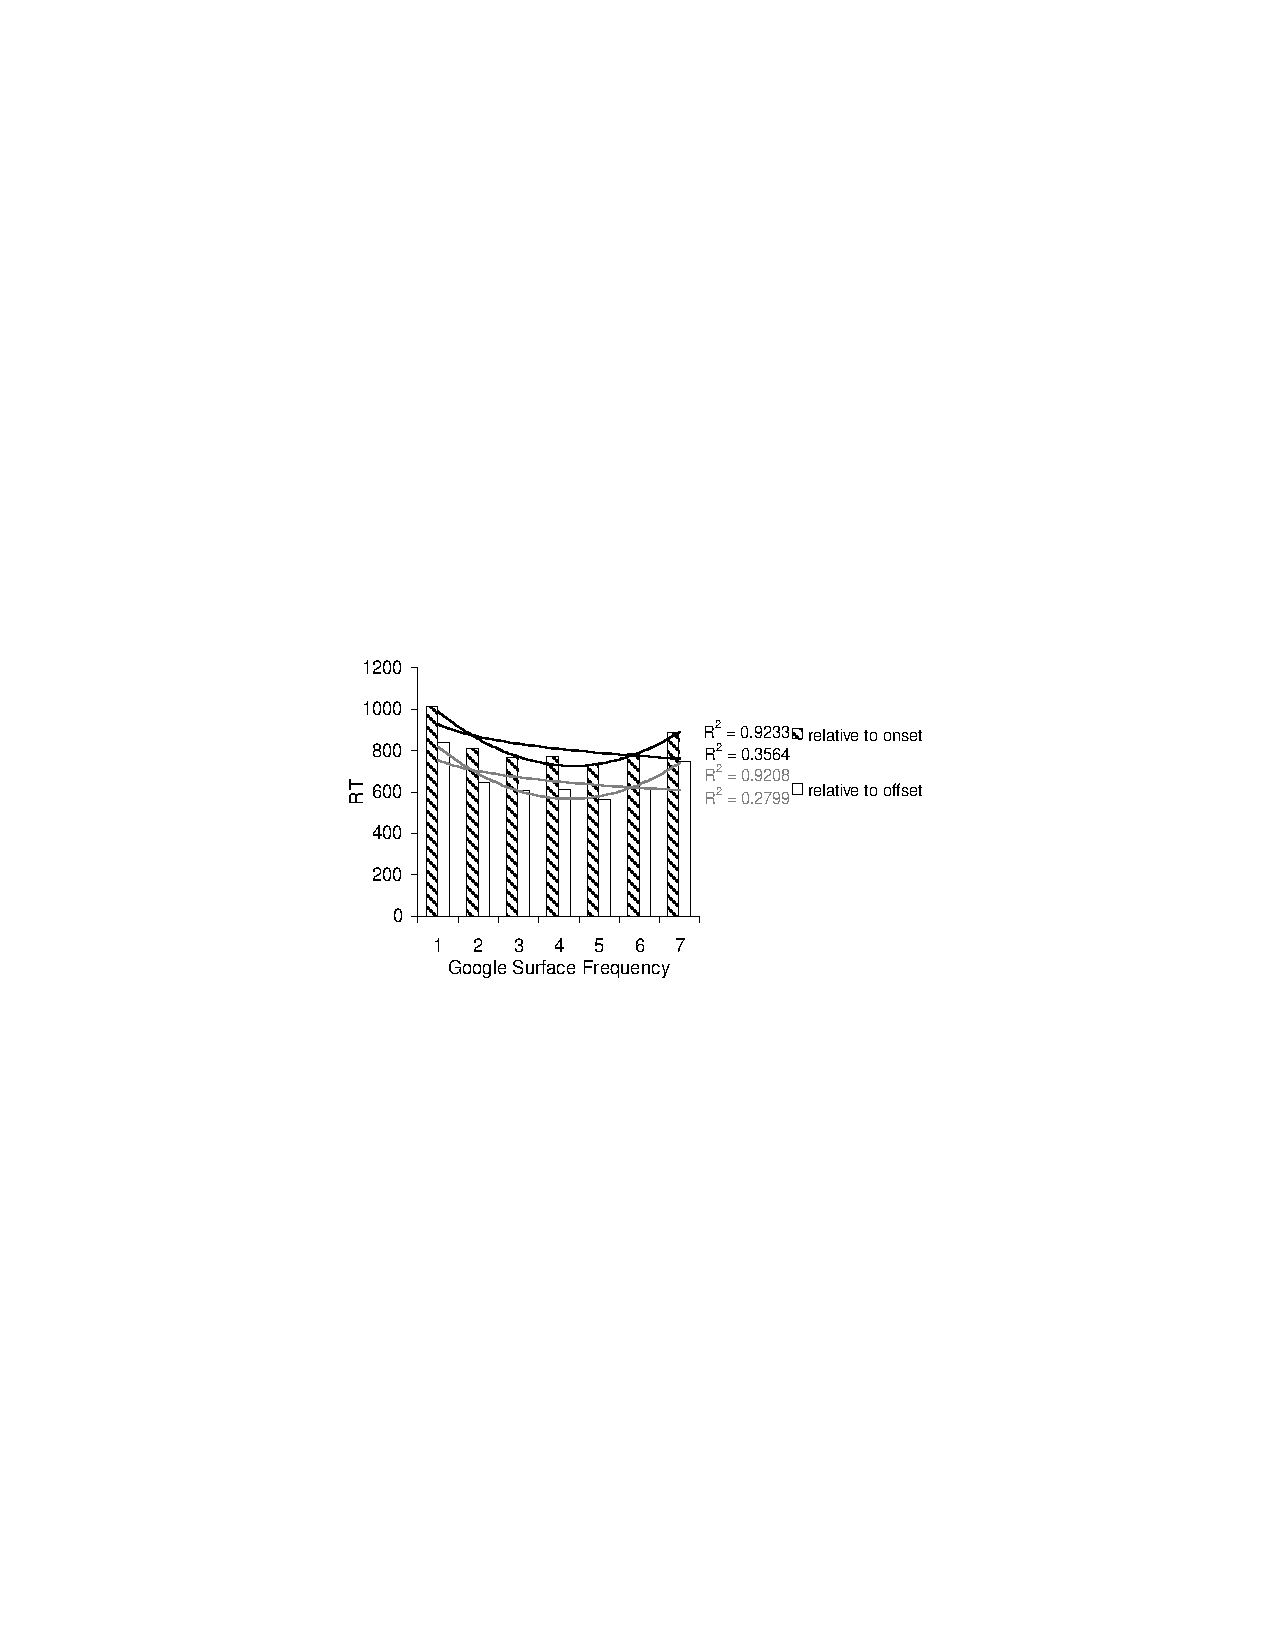
\includegraphics[width=1\linewidth,height=\textheight,keepaspectratio]{Chapters/Introduction/Figures/kapatsinskiradicke_graph.pdf}

}

\end{figure}%

A visualization of what this may look like is demonstrated in
Figure~\ref{fig-nointernalstructure}. The left tree represents the
phrase \emph{pick up} stored holistically but with intact internal
structure and the right tree represents the phrase \emph{pick up} stored
holistically but without internal structure.

\begin{figure}[htbp]

\caption{\label{fig-nointernalstructure}A visualization of a
holistically stored phrase with internal structure (left) and without
internal structure (right).}

\centering{

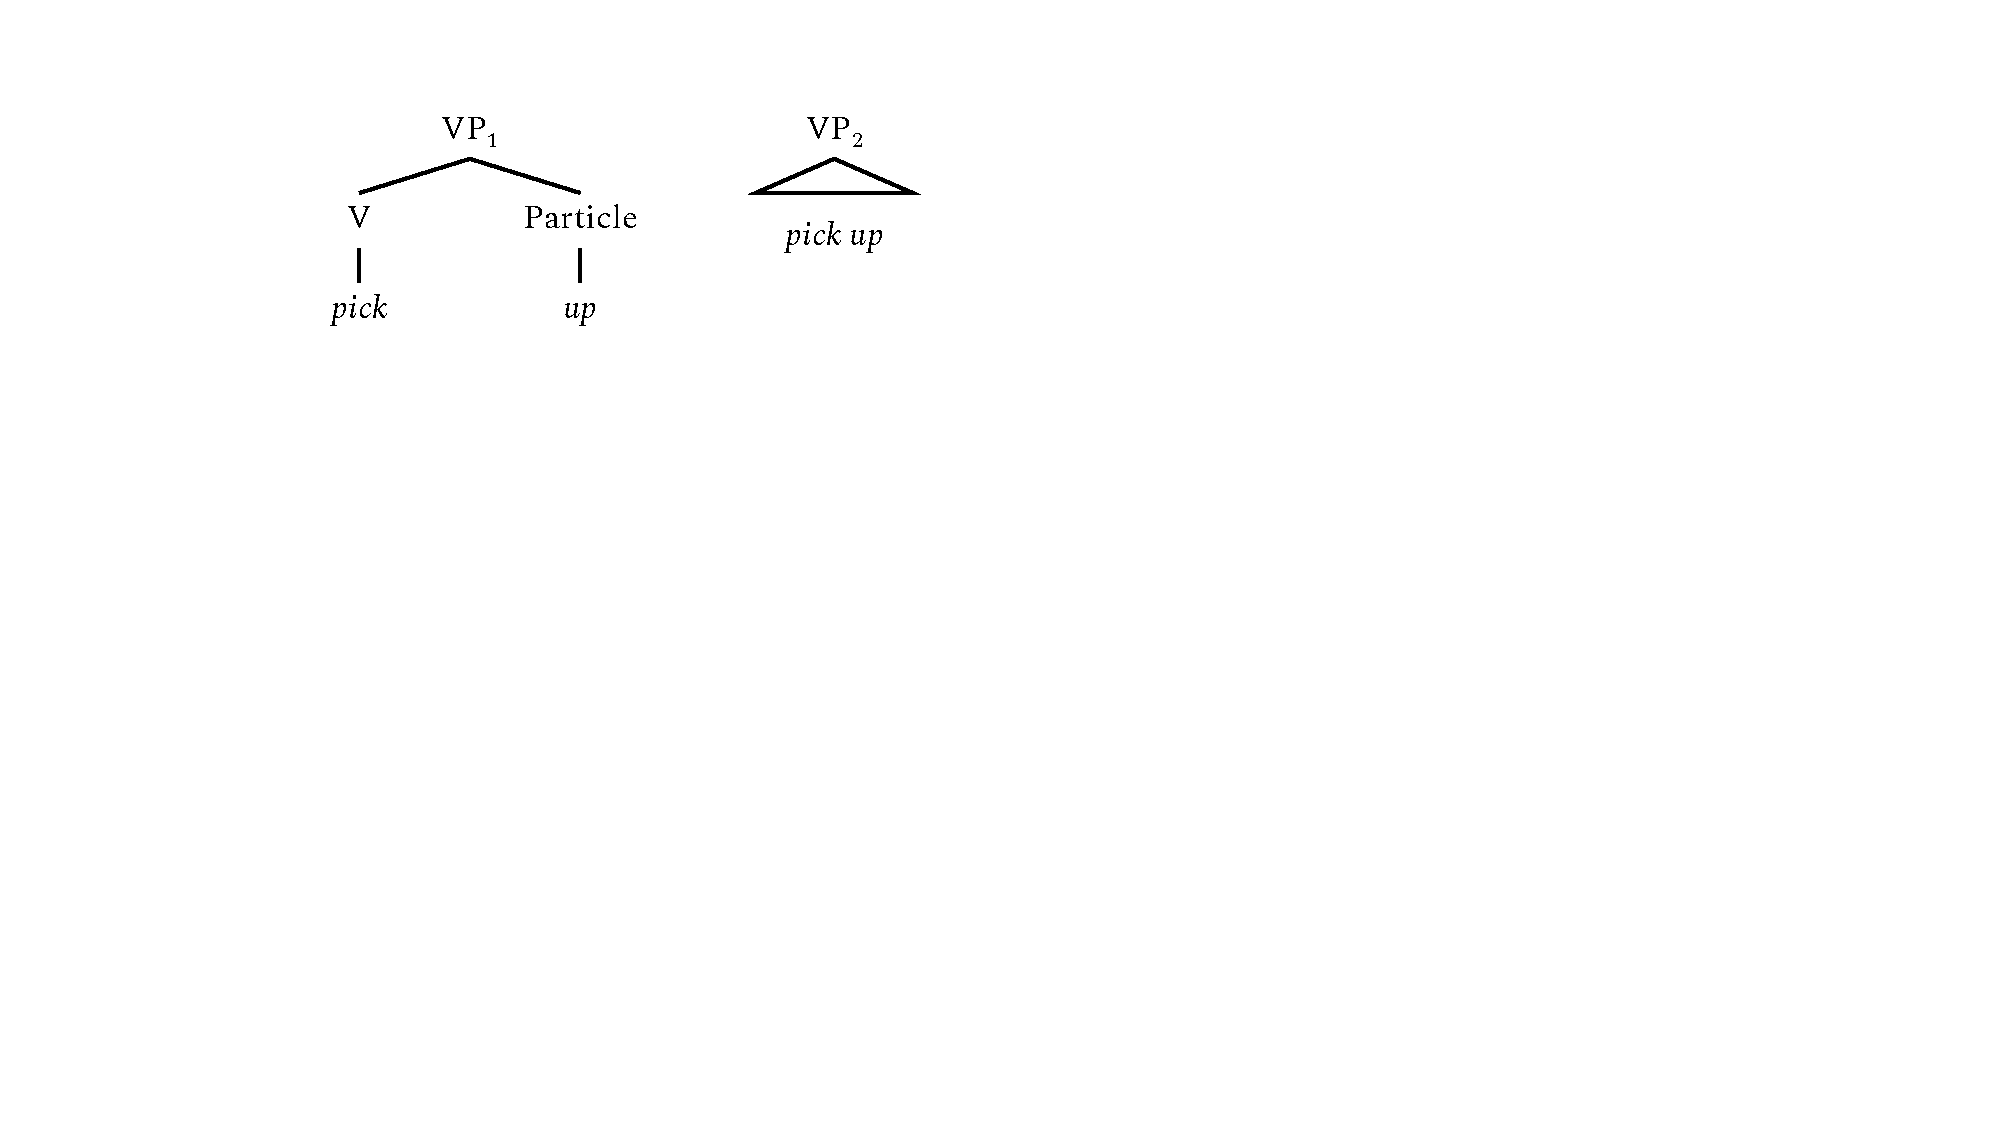
\includegraphics[width=0.6\linewidth,height=\textheight,keepaspectratio]{Chapters/Introduction/Figures/storage_syntax_tree.pdf}

}

\end{figure}%

This lack of internal structure could be lost over time, or it may
simply not have been learned in the first place. A great deal of
children's early learning is driven by memorizing chunks
(\citeproc{ref-bybee2003}{Bybee, 2003};
\citeproc{ref-tomaselloConstructingLanguageUsagebased2005}{Tomasello,
2005}). For example, Tomasello
(\citeproc{ref-tomaselloConstructingLanguageUsagebased2005}{2005})
argued that young children learn verbs in fixed ``islands'', producing
them in fixed-constructions before eventually learning to generalize
them to other contexts. As a result, children may be learning holistic
representations of them initially.

Additionally, if predictability drives word-segmentation, many
predictable phrases may be segmented out of the speech stream as a
single chunk. Following this, Bybee (\citeproc{ref-bybee2003}{2003})
argued that after learning these chunks, it seems unlikely that children
would then flush these from their memory. Further, many high frequency
and high predictability phrases have semantically vague relationships
(e.g., \emph{trick or treat}). These phrases may be difficult to
breakdown into their component words due to the lack of semantic
transparency. Children may learn to store these phrases holistically.
However, it is possible that their representations for these items are
updated to reflect knowledge of the individual words upon further
learning. Thus it is not entirely clear if holistically stored items
lack internal representations of the individual words.

On the other hand, internal structure could be lost over time. For
example, learners are more likely to semantically extend frequent forms
to novel contexts than infrequent forms
(\citeproc{ref-harmonPuttingOldTools2017}{Harmon \& Kapatsinski, 2017}).
This increase in accessibility may similarly drive their loss of
internal structure over time: as a phrase is extended to new contexts,
the representation of that phrase may also become more general to
accommodate the new context. This may lead to the internal structure
being lost over time as the contexts that the phrase is used in becomes
more different from the contexts in which the individual words are used.

\section{Processing Consequences of
Storage}\label{sec-processing-consequences-of-storage}

Speech is inherently temporally linear: unlike reading, when you hear a
sentence, you cannot skip forward or rewind back in time. As such, how
are holistically stored multi-word phrases processed? One possibility is
that when hearing part of the phrase, listeners may access the
representation for the holistically stored phrase. For example, in an
extreme case, hearing \emph{Habeas} may be enough to access the
representation of \emph{Habeas Corpus}.

However, this seems not to be the case. For example, Staub et al.
(\citeproc{ref-staubTimeCoursePlausibility2007}{2007}) examined the
effects of plausibility on the reading times of high frequency and low
frequency compound nouns (Noun and Noun compounds). Specifically,
participants read sentences that were either locally plausible or
locally implausible:

\begin{enumerate} 

    \item \textbf{Novel Compound}
    \begin{enumerate}
        \item[\textbf{1a}] The zookeeper picked up the monkey medicine that was in the enclosure.
        \item[\textbf{1b}] The zookeeper spread out the monkey medicine that was in the enclosure.
    \end{enumerate} \label{staubsentencenovel}
    \item \textbf{Familiar Compound}
    \begin{enumerate}
        \item[\textbf{2a}] Jenny looked out on the huge mountain lion pacing in its cage. \label{familiarplaus}
        \item[\textbf{2b}] Jenny heard the huge mountain lion pacing in its cage. \label{familiarimplaus}
    \end{enumerate} \label{staubsentencefamiliar}
\end{enumerate}

For example, Sentence 1a is locally plausible because the sentence is
plausible at the first noun. That is, \emph{picked up the monkey} is
plausible. On the other hand, 1b is locally implausible because it is
implausible at the first noun; \emph{spread out the monkey} is not
plausible. Sentences 2a and 2b are analogous but with a high frequency
compound noun.

Staub et al. (\citeproc{ref-staubTimeCoursePlausibility2007}{2007})
examined readers' eye-movements as they read these sentences and found
that for locally implausible sentences there was a slowdown at the first
noun. Crucially, this slowdown was equal for both the high and low
frequency compound nouns. However, if high frequency compound nouns are
stored holistically, and humans are able to access the representation at
the first noun, then participants should have been able to overcome at
least some of the slowdown due to the implausibility effect for the high
frequency items. However, this is not what Staub et al.
(\citeproc{ref-staubTimeCoursePlausibility2007}{2007}) found.

Given the results of Staub et al.
(\citeproc{ref-staubTimeCoursePlausibility2007}{2007}), one natural
possibility is that recognition happens incrementally and the
representation of the phrase becomes activated more strongly than the
words after the listener has heard each of the words in the phrase.
However, if this was the case then the results from Kapatsinski \&
Radicke (\citeproc{ref-kapatsinskiFrequencyEmergencePrefabs2009}{2009})
discussed earlier would complicate things. Recall that Kapatsinski \&
Radicke (\citeproc{ref-kapatsinskiFrequencyEmergencePrefabs2009}{2009})
found that participants are slower to recognize \emph{up} in high
frequency phrases. If recognition occurs incrementally, one would expect
that for high frequency phrases, \emph{up} would be recognized even
faster. That is, a slower recognition of \emph{up} in the context of
high-frequency phrases indicates that \emph{up} is harder to recognize
depending on what the preceding verb is. It's hard to see how an
incremental approach can account for this context-dependent difficulty
in recognition.

Following these results, it is possible that an incremental approach
with competition (such as one proposed by
\citeproc{ref-mcclellandTRACEModelSpeech1984}{McClelland et al., 1984})
may be the best account. Specifically, it is possible that processing
unfolds incrementally such that the representations of each individual
word are activated, however upon accessing the representation of the
phrase the word-level representations may be inhibited. For example,
upon hearing \emph{pick} perhaps the word-level representation for
\emph{pick} is activated, and upon hearing \emph{up} perhaps instead of
activating the representation for \emph{up}, the holistically stored
representation for \emph{pick up} is activated and the representations
at the word-level (\emph{pick} and \emph{up}) are inhibited. This
inhibition of \emph{up} maybe be the cause of the increased recognition
times for high-frequency V+\emph{up} compounds.

\section{Storage in Humans vs Large Language
Models}\label{sec-storage-in-humans-vs-large-language-models}

By now it should be clear that the literature has demonstrated that a
great deal of items are stored holistically. However it's unclear how
this can arise as a function of learning. In order to help address this
question, we turn to large language models, which have developed rapidly
over the last several years.

\subsection{Transformer Model
Architecture}\label{transformer-model-architecture}

When I started this program in 2020, the idea of a single language model
that could produce fluent text that was discernible from text written by
humans seemed like a far-off dream. However, with rapid advancements in
transformer models, the language models of today have seemed to
accomplish that goal. With their rapid advancement, the question of
whether they may be accomplishing this goal in a similar manner as
humans has been at the forefront of a great deal of linguistics and
cognitive science research. Thus in this section, we will introduce the
transformer architecture along with the current state of the literature
on their ability to store and learn generalized knowledge.

The term large language model typically refers to a transformer model
(\citeproc{ref-vaswaniAttentionAllYou2017}{Vaswani et al., 2017}), such
as Llama (\citeproc{ref-touvronLlama2Open2023}{Touvron et al., 2023}).
The heart and soul of the transformer model is a feed-forward neural
network (Figure~\ref{fig-neuralnet}). These models typically take
token-level embeddings as their input and try to predict the next token.
For example, if the model is presented with the input \emph{The boy went
outside to fly his \_\_\_\_\_}, the large language model may assign high
probabilities to the output tokens \emph{kite} or
\emph{airplane}.\footnote{Technically, the token-level of large language
  models is not analogous to words. For example, GPT-2's tokenizer
  tokenizes \emph{kite} into two tokens: \emph{k}, and \emph{ite}. As
  such, GPT-2 assigns a high probability to \emph{k} as the upcoming
  token in that context.}

\begin{figure}[htbp]

\caption{\label{fig-neuralnet}A visualization of a feed-forward neural
network.}

\centering{

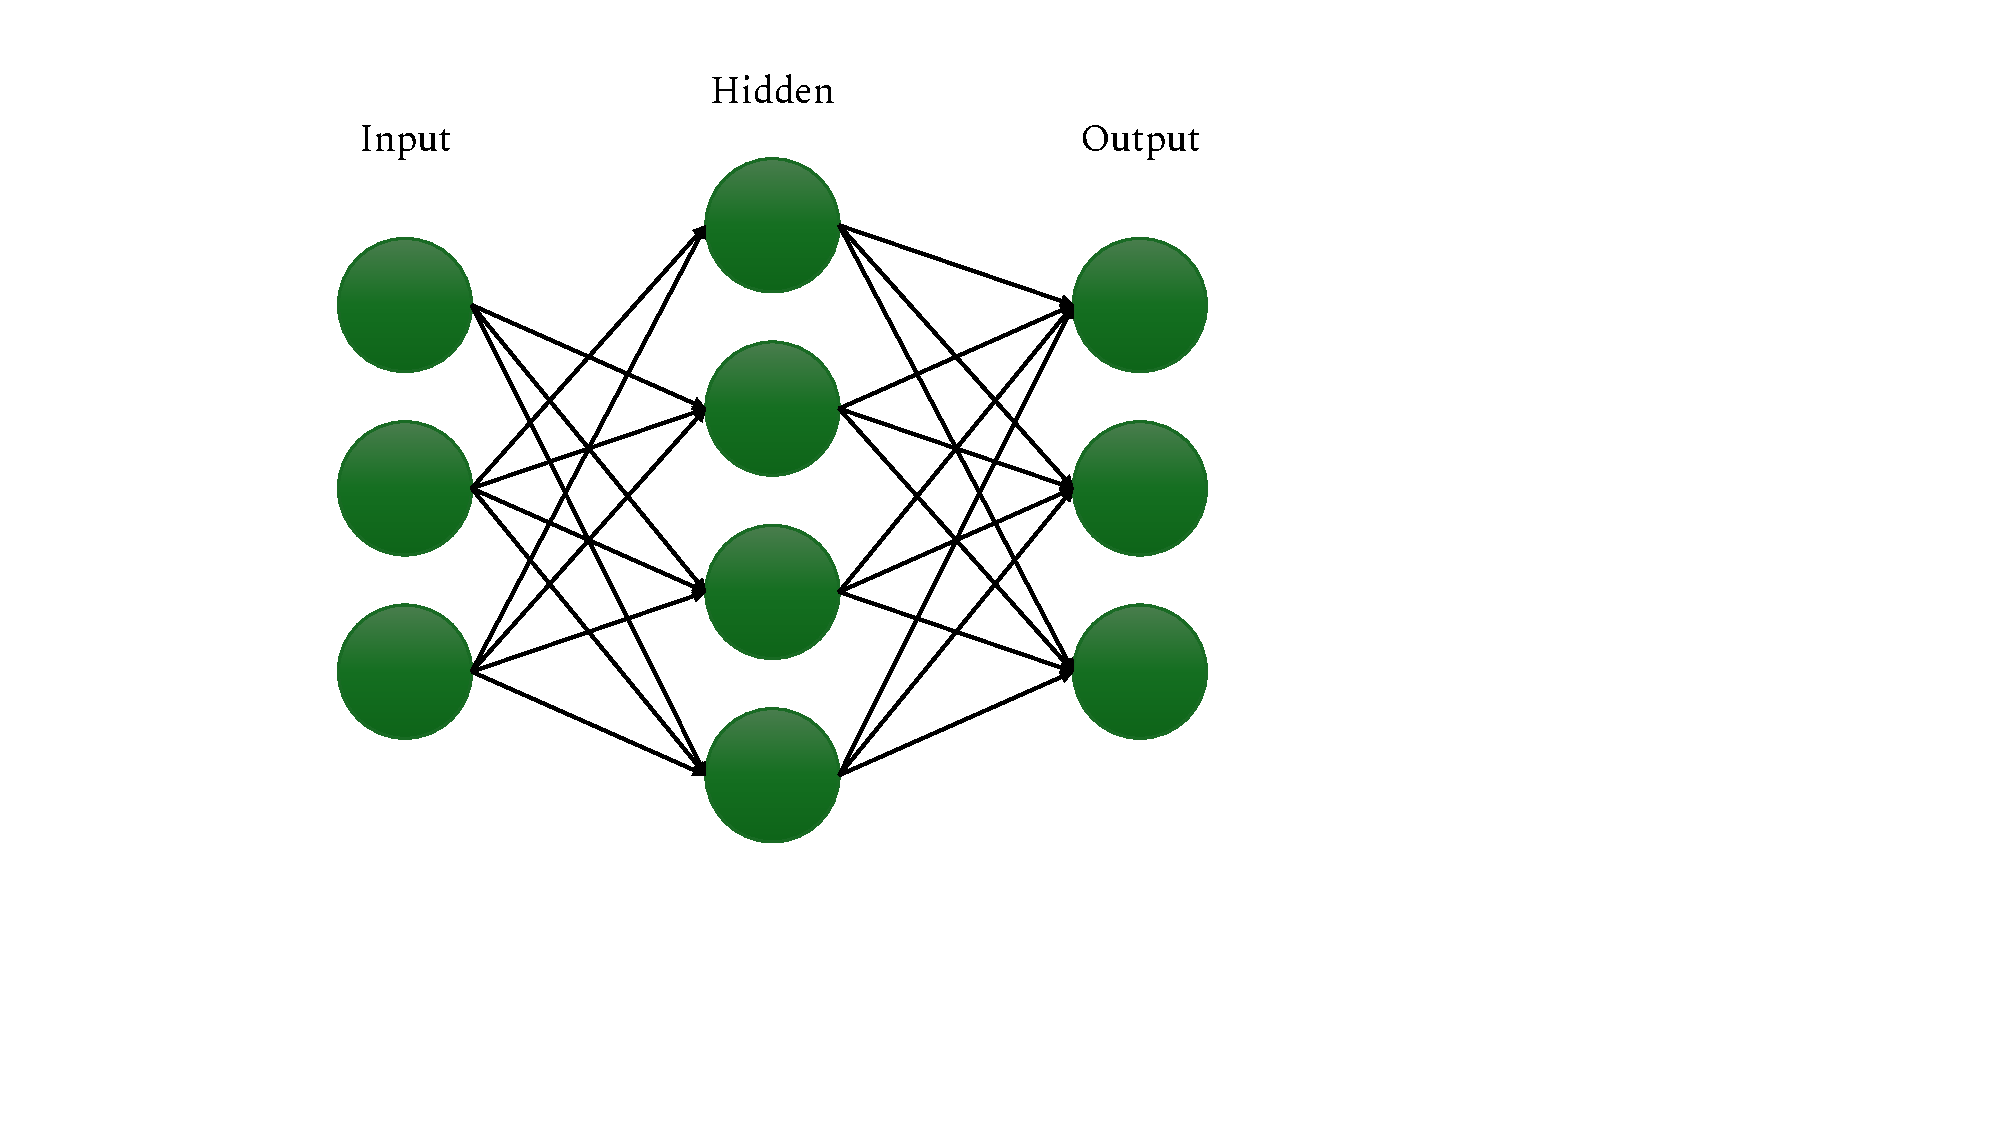
\includegraphics[width=0.7\linewidth,height=\textheight,keepaspectratio]{Chapters/Introduction/Figures/feed-forward neural network visualization.pdf}

}

\end{figure}%

In addition to a feed-forward neural network, the transformer
architecture also includes a self-attention mechanism. Self-attention
helps the model learn which words are related to each other, which has
been a driving factor in the success of the transformer model over its
predecessors. For example, previous models such as Long-Short Term
Memory (LSTM) models or Recurrent Neural Network (RNN) models struggled
with long-term dependencies
(\citeproc{ref-al-selwiLSTMInefficiencyLongterm2023}{Al-Selwi et al.,
2023}; \citeproc{ref-bengioProblemLearningLongterm1993}{Bengio et al.,
1993}). The self-attention mechanism was one of the solutions proposed
to address this difficulty. The self-attention mechanism is a way to
quantify which words are most related to each other. Specifically, the
self-attention mechanism computes the strength of the relationship of
each pair of words in the sentences
(\citeproc{ref-vaswaniAttentionAllYou2017}{Vaswani et al., 2017}). Thus
in the sentence, \emph{the students that go to school are bright}, the
self-attention mechanism would assign a high value to the pair
\{\emph{students, are\}} because the word \emph{students} is very
relevant for predicting \emph{are} (as opposed to \emph{is}).

The full transformer model architecture is presented in
Figure~\ref{fig-transformermodel}, reproduced from Vaswani et al.
(\citeproc{ref-vaswaniAttentionAllYou2017}{2017}).

\begin{figure}[htbp]

\caption{\label{fig-transformermodel}The transformer model architecture,
reproduced from Vaswani et al.
(\citeproc{ref-vaswaniAttentionAllYou2017}{2017}).}

\centering{

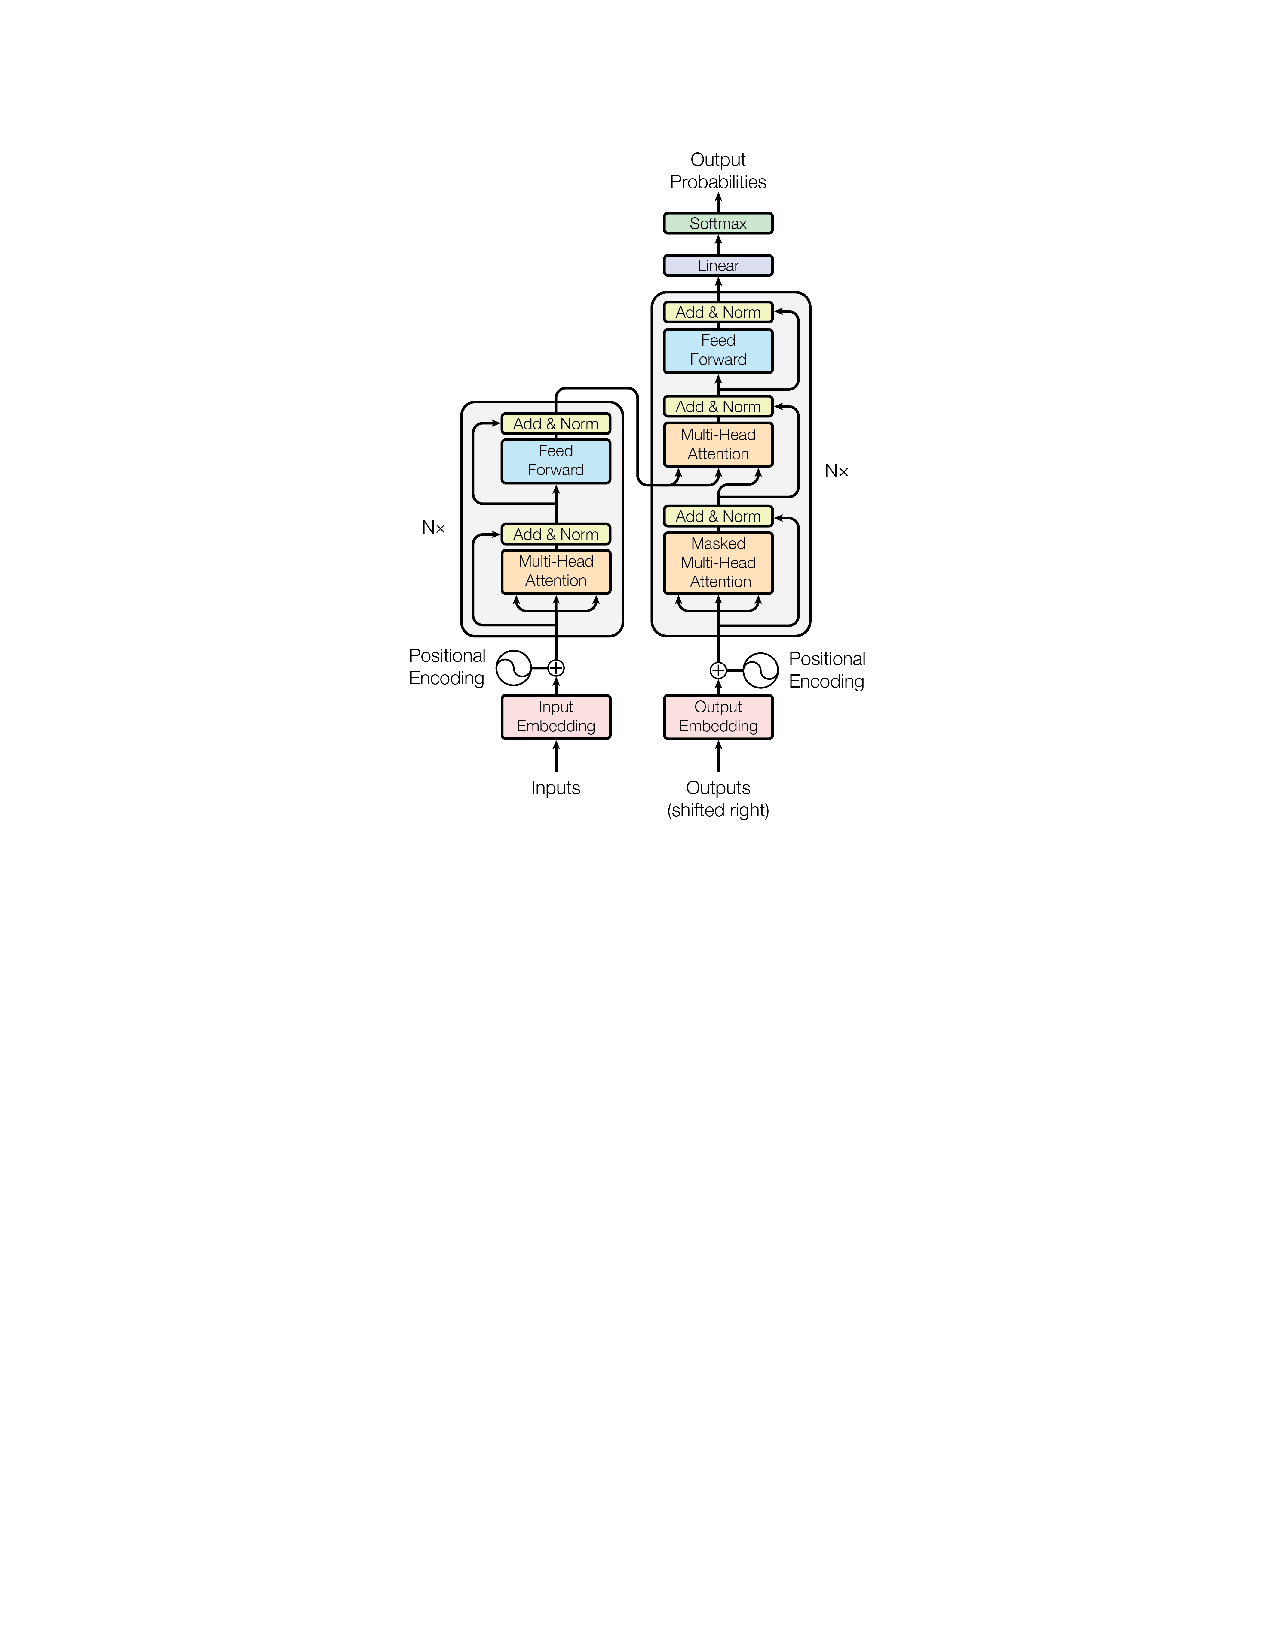
\includegraphics[width=1\linewidth,height=\textheight,keepaspectratio]{Chapters/Introduction/Figures/transformer-architecture.pdf}

}

\end{figure}%

\subsection{Lessons from Transformer
Models}\label{lessons-from-transformer-models}

Transformer models have achieved state-of-the-art performance on many
benchmarks and are undoubtedly able to produce fluent, human-like text.
However, it remains unclear to what extent they do this in a human-like
manner. Specifically, how much are these models simply memorizing as
opposed to learning something more abstract about the language?

On one hand, modern large language models are trained on trillions of
tokens of data
(\citeproc{ref-groeneveldOLMoAcceleratingScience2024}{Groeneveld et al.,
2024}). This is magnitudes larger than humans, who have heard an average
of 350 million words by the time they enter college
(\citeproc{ref-levyProcessingExtraposedStructures2012}{Levy et al.,
2012}). Due to the size of the training data, there has been a lot of
skepticism about how much they're actually learning and how much they're
simply parroting from the training data
(\citeproc{ref-benderDangersStochasticParrots2021}{Bender et al.,
2021}). This skepticism is furthered by the fact that a lot of the
training data for high-end large language models is either not
open-access, or so huge that it is difficult to work with.

Further, there is evidence that large language models do copy a decent
amount from their training. For example, Haley
(\citeproc{ref-haleyThisBERTNow2020}{2020}) demonstrated that many of
the BERT models are not able to reliably determine the correct plural
form for novel words. Similarly, Li \& Wisniewski
(\citeproc{ref-liAreNeuralNetworks2021}{2021}) demonstrated that BERT
relies on memorization when producing the correct tense for a word as
opposed to learning a more general linguistic pattern.

However, there is also a substantial amount of evidence that language
models are learning more general patterns of the language
(\citeproc{ref-lasriSubjectVerbAgreement2022}{Lasri et al., 2022};
\citeproc{ref-liAssessingCapacityTransformer2023}{Li et al., 2023};
\citeproc{ref-liAreNeuralNetworks2021}{Li \& Wisniewski, 2021};
\citeproc{ref-mccoyHowMuchLanguage2023}{McCoy et al., 2023};
\citeproc{ref-misraLanguageModelsLearn2024}{Misra \& Mahowald, 2024};
\citeproc{ref-weissweilerLinguisticGeneralizationsAre2025}{Weissweiler
et al., 2025}; \citeproc{ref-yaoBothDirectIndirect2025}{Yao et al.,
2025}). For example, Lasri et al.
(\citeproc{ref-lasriSubjectVerbAgreement2022}{2022}) examined whether
BERT is able to use the correct inflection of verbs in semantically
incoherent contexts (e.g., \emph{colorless green ideas sleep
furiously}). They found that while BERT does do worse when the context
is semantically incoherent, the decrease in performance is comparable to
the decrease we see in humans.

Additionally, Li et al.
(\citeproc{ref-liAssessingCapacityTransformer2023}{2023}) examined
BERT's performance on subject-verb and object-past agreements in French.
They found that BERT uses abstract knowledge to predict subject-verb and
object-past agreements.

There is also evidence that other transformer models can learn more
abstract knowledge as well. For example, McCoy et al.
(\citeproc{ref-mccoyHowMuchLanguage2023}{2023}) examined the text that
GPT-2 produces in relation to its training data. They found that while
GPT-2 does copy a great deal, it also produces both novel words and
syntactic structures.

More recently, there has been an interesting line of research examining
language models trained on a more human amount of data. For example,
Misra \& Mahowald (\citeproc{ref-misraLanguageModelsLearn2024}{2024})
demonstrated that a language model trained on the BabyLM-strict corpus
(\citeproc{ref-warstadtFindingsBabyLMChallenge2023}{Warstadt et al.,
2023}) (a corpus containing a comparable amount of data as humans
receive) can learn article-adjective-numeral-noun constructions (AANNs).
AANNs are constructions such as \emph{a beautiful five days}. They occur
relatively infrequently in English but humans still learn natural
preferences for these. For example, while \emph{a beautiful five days}
is perfectly grammatical, \emph{a blue five pencils} is not. They found
that even after removing all AANN occurrences from the training data,
the large language model is still able to learn these constructions.
They further demonstrated that this is likely learned from similar
constructions, such as \emph{a few days}. The results of this show that
even when trained on a comparable amount of data as humans, language
models are still able to learn general patterns in the language.

Similarly, Yao et al. (\citeproc{ref-yaoBothDirectIndirect2025}{2025})
examined how language models learn the dative alternation. The dative
alternation is a common construction in English where one can say either
\emph{give X to Y} or \emph{give Y X}. Humans have preferences for these
such as a length and an animacy preference. They trained a language
model on a comparable amount of data to humans. Crucially they removed
dative alternations that contained a length or animacy bias. They found
that while the effect weakens, there is still an effect of length. They
argued that this is evidence that language models are learning general
patterns of the language. These results taken together with previous
results demonstrate the ability of transformer models to learn general
patterns in the language.

However, there is still a lot we don't know. What factors determine
whether models learn general patterns of the language as opposed to
relying on item-specific preferences? For example, humans seem to be
sensitive to a combination of type and token frequency when they
generalize beyond a specific word
(\citeproc{ref-harmonPuttingOldTools2017}{Harmon \& Kapatsinski, 2017}).
Are language models sensitive to similar factors? Further is this
knowledge represented in a similar way as humans? That is, are the
general preferences that large language models learn similar to those
that humans learn? Understanding the answers to these questions is
important for evaluating these models as theories of human language
learning.

\section{Outline of Dissertation}\label{sec-outline-of-dissertation}

In the present dissertation, we provide an in depth examination of how
humans trade off between storage and computation. In the next chapter,
we examine whether predictability drives storage and how holistic
representations are accessed. In Chapter 3, we examine how holistically
stored items are represented. Chapter 4 examines how large language
models trade off between storage and computation. Chapter 5 examines how
stored items are represented in large language models. Chapter 6
examines whether storage accounts can explain frequency-dependent
preference extremity. Finally, Chapter 7 examines a novel prediction
found in Chapter 6.

\bookmarksetup{startatroot}

\chapter{Does Predictability Drive the Holistic Storage of Compound
Nouns?}\label{does-predictability-drive-the-holistic-storage-of-compound-nouns}

\section{Introduction}\label{introduction-1}

Learning a language is not a trivial task. In order to be successful,
learners must accurately segment the continuous speech stream into
smaller segments, including phrases, words, morphemes, and phonemes. One
of the main questions that arises out of this task is what exactly is
the size of the units that learners are storing? That is, are they
storing individual words, entire sentences, phrases, or some combination
of all of these? One possibility is that learners store very little
outside of words and idioms. For example, traditional theories have
argued that learners don't store any more than they need to: they store
only what they can't form compositionally using a set of rules, and
generate everything else (e.g., \citeproc{ref-chomsky1965}{Chomsky,
1965}). For example, inflected words, such as \emph{walked} would be
generated by accessing the stored root, \emph{walk}, and then applying a
past tense rule that generates \emph{walked} from the root. Similarly, a
phrase like \emph{I don't know} would be generated by accessing each of
the individually stored words \emph{i}, \emph{don't}, and \emph{know}.

On the opposite side of this theoretical spectrum, another possibility
is that learners store everything, including entire sentences. Ambridge
(\citeproc{ref-ambridgeStoredAbstractionsRadical2020}{2020}) argued for
exactly this, specifically arguing that everything a learner hears ``is
stored with its meaning, as understood in that individual situation''
and that unwitnessed novel-forms are produced using on-the-fly analogy
across stored exemplars Ambridge
(\citeproc{ref-ambridgeStoredAbstractionsRadical2020}{2020}). For
example, producing a novel plural form, like \emph{wugs}, would consist
of analogizing (on-the-fly) over multiple stored exemplars (e.g.,
\emph{cats}, \emph{chairs}, \emph{dogs}, etc).

It is also possible that what gets stored is somewhere in between these
two extremes. For example, usage-based construction grammar approaches
have posited that a lot more than just words are stored -- including
high frequency phrases -- but rather than storing everything, or storing
only the most basic units, that storage is driven by usage
(\citeproc{ref-arnonMoreWordsFrequency2010}{Arnon \& Snider, 2010};
\citeproc{ref-baayenAmorphousModelMorphological2011}{R. H. Baayen et
al., 2011}; \citeproc{ref-bybee2003}{Bybee, 2003};
\citeproc{ref-bybee2001}{Bybee \& Hopper, 2001};
\citeproc{ref-goldbergConstructionsNewTheoretical2003}{Goldberg, 2003};
\citeproc{ref-morgan2015}{Morgan \& Levy, 2015b},
\citeproc{ref-morganAbstractKnowledgeDirect2016}{2016a},
\citeproc{ref-morgan2024}{2024};
\citeproc{ref-odonnellProductivityReuseLanguage2016}{O'Donnell, 2016};
\citeproc{ref-tomaselloConstructingLanguageUsagebased2005}{Tomasello,
2005}). That is to say, the size of the units stored is driven by the
statistical distribution of the language that the learner is producing
and perceiving. For example, Bybee (\citeproc{ref-bybee2003}{2003}) drew
an analogy to learning to play a piece on the piano:

\begin{quote}
An important result of learning to play several pieces is that new
pieces are then easier to master. Why is this? I hypothesize that the
player can access bits of old stored pieces and incorporate them into
new pieces. The part of a new piece that uses parts of a major scale is
much easier to master if the player has practiced scales than is a part
with a new melody that does not hearken back to common sequences. This
means that snatches of motor sequences can be reused in new contexts.
The more motor sequences stored, the greater ease with which the player
can master a new piece.
\end{quote}

\noindent In this same line of thinking, Bybee
(\citeproc{ref-bybee2003}{2003}) further argued against a strictly
traditional view, stating that learning the English past tense
\emph{-ed} requires learning a series of words that contain that segment
(e.g., \emph{played}, \emph{spilled}, \emph{talked}) and that these are
not necessarily flushed from memory after learning the English past
tense marker.

There is no shortage of evidence for the holistic storage of multi-word
phrases. For example, high-frequency phrases, such as \emph{I don't
know}, have been shown to undergo phonetic reduction that isn't seen in
other low or mid-frequency phrases containing \emph{don't}
(\citeproc{ref-bybeeEffectUsageDegrees1999}{Bybee \& Scheibman, 1999})
suggesting that the representation of \emph{I don't know} is separate
from the representation of each of the individual words. In other words,
the susceptibility of high-frequency phrases to phonological change is
strong evidence that they may come to have a mental representation for
the whole expression (i.e., holistic storage). This example is not an
outlier either, there are many examples of high-frequency phrases
undergoing phonetic reduction: \emph{going to}, want to\emph{, have to},
etc (\citeproc{ref-bybee2003}{Bybee, 2003}). In Korean, Yi
(\citeproc{ref-yiEumun2002}{2002}) demonstrated that in multi-word
phrases containing the adnominal future marker (\emph{-l}), the
tensification of the consonant following the adnominal is predicted by
the phrasal frequency. That is, in high-frequency phrases, consonants
following the adnominal became tense at a higher rate than in
low-frequency phrases.\footnote{A similar effect has been demonstrated
  on the word-level as well in Korean, where epenthesis has been
  documented to occur more often in high-frequency words than in
  low-frequency words
  (\citeproc{ref-leeFrequencyEffectsMorphologisation2015}{Lee \&
  Kapatsinski, 2015}). This suggests that there may not be a clear
  division between the representation of high-frequency phrases and
  high-frequency words.}

Evidence for holistic storage is not limited to phonological effects,
either. In the Psycholinguistics literature, Siyanova-Chanturia et al.
(\citeproc{ref-siyanova-chanturiaSeeingPhraseTime2011}{2011})
demonstrated that readers are sensitive to the ordering of binomials in
English. In an eye-tracking experiment, participants read frequent
binomial expressions in English in their preferred order (e.g.,
\emph{bride and groom}) and their reversed order (\emph{groom and
bride}). They found that the preferred orderings were read faster.
Further, Morgan \& Levy
(\citeproc{ref-morganAbstractKnowledgeDirect2016}{2016a}) investigated
whether the results from Siyanova-Chanturia et al.
(\citeproc{ref-siyanova-chanturiaSeeingPhraseTime2011}{2011}) could be
attributed to abstract knowledge of binomial orderings (e.g., a
preference for male names before female names) or whether they were due
to participants' direct experience with those items (e.g., hearing one
ordering of a specific binomial more often than the complementary
ordering). They developed a probabilistic model to approximate native
English speakers' ordering preferences and combined that with a
forced-choice and a self-paced reading task in order to investigate
whether ordering preferences were driven by abstract knowledge or direct
experience of the expression. They found that reading times for frequent
binomials were influenced only by relative frequency (i.e., direct
experience), not abstract knowledge. That is to say, ordering
preferences of frequent binomials weren't explained by abstract ordering
preferences, but rather by linguistic experience with the specific
binomial, suggesting that high-frequency binomials are stored
holistically.

Similarly, O'Donnell
(\citeproc{ref-odonnellProductivityReuseLanguage2016}{2016}) tested 4
probabilistic models on their ability to learn the English past tense
and derivational morphology. Specifically, they tested a Full-parsing
model, which stores minimal-sized units only, a Full-listing model,
which stores the entirety of units only, an Exemplar-based model, which
stores all units and all sub-units consistent with the data, and finally
a Productivity as an Inference model, which, similar to the
Exemplar-based Inference model, can store both smaller and larger
structures, but probabilistically determines which items to store based
on the data. They found that the Inference-based model performed the
best overall for both past tenses and derivational morphology. In other
words, storing units of varying sizes (as opposed to just minimal or
maximal-sized units) seems to be the most conducive to learning the
various morphological paradigms in English.

Despite the clear evidence for the holistic storage of some multi-word
units, however, it is still largely unclear what determines whether a
unit is stored holistically. For example, it is possible that storage is
driven by either \textbf{phrasal frequency}
(\citeproc{ref-bybee2001}{Bybee \& Hopper, 2001}) or by the mutual
\textbf{predictability} of a phrase's component parts {[}i.e., how
predictable the whole phrase is from part of the phrase; O'Donnell
(\citeproc{ref-odonnellProductivityReuseLanguage2016}{2016}){]}. For
example, as previously stated, there is an abundance of evidence that
high-frequency phrases are more susceptible to phonetic reduction than
low-frequency phrases (\citeproc{ref-bybee2003}{Bybee, 2003};
\citeproc{ref-bybeeEffectUsageDegrees1999}{Bybee \& Scheibman, 1999}).
Additionally, high-frequency phrases have been shown to lose the
recognizability of their component parts relative to low-frequency
phrases
(\citeproc{ref-kapatsinskiFrequencyEmergencePrefabs2009}{Kapatsinski \&
Radicke, 2009}). For example, \emph{up} is harder to recognize in
\emph{pick up} than in \emph{run up}. On the other hand, in the learning
literature, there is significant evidence that learning is driven by
prediction error as opposed to raw co-occurrence statistics. For
example, Ramscar et al.
(\citeproc{ref-ramscarChildrenValueInformativity2013}{2013})
demonstrated that in word learning, children rely on more than simple
co-occurrence statistics but also on how \emph{informative} -- that is,
how \emph{predictive} -- a cue is of an outcome (relative to other
cues). Specifically, they demonstrated that children rely on not only
co-occurrence rate, but also background rate (how often a cue is present
without an outcome). In other words, assuming doors have a higher
co-occurrence rate and lower background rate than all the other
competing cues (e.g., brown, house, room) for the word \emph{door}, then
children will learn that doors are the best predictor of the word
\emph{door}
(\citeproc{ref-ramscarChildrenValueInformativity2013}{Ramscar et al.,
2013}).

A similar debate persists in the speech perception literature, where
Pierrehumbert
(\citeproc{ref-pierrehumbertExemplarDynamicsWord2001}{2001}) argued that
internal representations reflect the raw frequency distribution of the
input. On the other hand, Olejarczuk et al.
(\citeproc{ref-olejarczukDistributionalLearningErrordriven2018}{2018})
argued that the learning of phonemes is driven not by co-occurrence
statistics (i.e., raw frequency), but rather by surprisal (i.e.,
prediction error). In other words, learners are actively predicting
upcoming phonemes and update their beliefs in proportion to how
surprising the upcoming phoneme is. Thus the debate between
co-occurrence vs predictability in the role of learning is not unique to
the word learning literature.

Additionally, if learners are storing more than just single-word units,
what are the processing consequences of this? For example, as mentioned
earlier, Kapatsinski \& Radicke
(\citeproc{ref-kapatsinskiFrequencyEmergencePrefabs2009}{2009})
investigated the recognition of the particle \emph{up} in phrases of
varying frequencies and found that the recognition of the particle
\emph{up} is significantly more difficult in a high-frequency phrases
than in low frequency phrases, suggesting that high frequency units
`fuse' together, losing some of the recognizability of their individual
parts.

On the other hand, Staub et al.
(\citeproc{ref-staubTimeCoursePlausibility2007}{2007}) investigated the
effects of plausibility on the reading times of familiar and novel
compound nouns, which were compound nouns with high and low phrasal
frequency respectively. Participants read sentences which contained a
novel compound noun or a familiar compound noun (See the sentences
below) in a plausible condition (a) or an implausible condition (b).
Crucially, the second noun in the compound eliminated the local
implausibility such that every sentence was plausible after reading the
second noun. For example, in 1b \emph{The zookeeper spread out the
monkey\ldots{}} is locally implausible, however upon reading the second
noun in the compound, \emph{medicine}, the local implausibility is
eliminated.

\begin{enumerate} 

    \item \textbf{Novel Compound}
    \begin{enumerate}
        \item[\textbf{1a}] The zookeeper picked up the monkey medicine that was in the enclosure.
        \item[\textbf{1b}] The zookeeper spread out the monkey medicine that was in the enclosure.
    \end{enumerate} \label{staubsentencenovel}
    \item \textbf{Familiar Compound}
    \begin{enumerate}
        \item[\textbf{2a}] Jenny looked out on the huge mountain lion pacing in its cage. \label{familiarplaus}
        \item[\textbf{2b}] Jenny heard the huge mountain lion pacing in its cage. \label{familiarimplaus}
    \end{enumerate} \label{staubsentencefamiliar}
\end{enumerate}

\noindent They found that the size of the plausibility effect was the
same for both novel and familiar compound nouns. That is to say, while
familiar items were read more quickly than novel items, and there was an
increase in reading times in the implausible condition, the size of the
plausibility effect was not different for familiar items (relative to
novel items). However, if familiar items are stored holistically, one
might expect that readers would predict the second noun upon reading the
first, thus eliminating the local implausibility. Thus, if these items
are stored holistically it begs the question of what the processing
consequences of storage are. On the other hand, it may just be that
these items are not stored. For example, it is possible that, as has
been previewed throughout the introduction, phrasal frequency may not be
the driving factor of storage and that it is actually predictability
that might be driving storage. If this is the case, then it is possible
that the reason for a lack of an interaction effect in Staub et al.
(\citeproc{ref-staubTimeCoursePlausibility2007}{2007})'s results is due
to their stimuli being low predictability compound nouns. For example,
while \emph{mountain lion} has a high phrasal frequency, \emph{mountain}
is not very predictable of \emph{lion} (that is, the probability of
\emph{lion} following \emph{mountain} is fairly low, despite the overall
phrase having a relatively high frequency).

Thus there are two main problems that the present study aims to provide
insight on: what exactly drives holistic storage, and what are the
processing consequences of storage? In Experiment 1, we first replicate
Staub et al. (\citeproc{ref-staubTimeCoursePlausibility2007}{2007})'s
experiment using a maze task (\citeproc{ref-boyceMazeMadeEasy2020}{Boyce
et al., 2020}). In Experiment 2, we use the same methodology, but
instead of using high (phrasal) frequency compound nouns, we use high
\emph{predictability} compound nouns (e.g., \emph{peanut butter}). By
using the highest predictability compound nouns from the google
\emph{n}-grams corpus {[}Michel et al.
(\citeproc{ref-michel2011quantitativeanalysisculture}{2011}), we ask
whether the difference in reaction times between the locally implausible
and plausible contexts differs depending on whether the compound noun is
highly predictable or not. For example, if highly predictable compound
nouns are stored holistically, it is possible that when listeners hear,
or read, the first noun in a highly predictable compound noun they may
access the second noun as well and/or a holistic compound noun
representation. If this is the case, then locally implausible contexts
should not incur as much processing difficulty when the compound noun is
highly predictable because the second noun eliminates the local
implausibility. Lastly in Experiments 3 and 4 we replicate these with
eye-tracking.

\section{Experiment 1}\label{experiment-1}

\subsection{Methods}\label{methods}

\subsubsection{Participants}\label{participants}

Participants were presented with sentences online via ibex farm, a
web-based experiment software platform that is freely-available
(\url{github.com/addrummond/ibex}) and were recruited through the
University of California Linguistics/Psychology Human Subjects Pool. To
prevent selection bias, participants signed up for the experiment
blindly, without knowledge of the content of the experiment. 146
participants were recruited, however 30 participants were excluded for
having an overall accuracy below 70\% (in this case, accuracy is
operationalized as choosing the correct word; an inaccuracy would be
choosing the ungrammatical distractor word), leaving a total of 116
participants. All participants self-reported being native English
speakers.

\subsubsection{Stimuli}\label{stimuli}

The experimental sentences were sentences containing compound nouns from
(\citeproc{ref-staubTimeCoursePlausibility2007}{Staub et al., 2007})
which varied upon two dimensions: local plausibility and familiarity.
Locally plausible sentences were sentences in which the reading at the
first noun was plausible and locally implausible sentences were
sentences in which the reading at the first noun in the compound was
implausible (see example sentences \ref{staubsentencenovel} and
\ref{staubsentencefamiliar}). Local plausibility was a within-item
effect and familiarity (the frequency of the compound noun) was a
between-item effect. Examples \ref{staubsentencenovel} and
\ref{staubsentencefamiliar} above exemplify each condition: the first
sentence in each is locally plausible while the second one is locally
implausible. For example, in sentence
\hyperref[staubsentencefamiliar]{2a}, it is semantically plausible that
\emph{Jenny looked out on the huge mountain\ldots{}} but not
semantically plausible that \emph{Jenny heard the huge mountain}
(\hyperref[staubsentencefamiliar]{2b}). Altogether, our stimuli
consisted of 24 novel items, 24 familiar items {[}taken from Staub et
al. (\citeproc{ref-staubTimeCoursePlausibility2007}{2007}){]}, and 188
filler sentences in order to avoid participants discerning the
experimental design.

\subsubsection{Procedure}\label{procedure}

Experiment 1 is a direct replication of Staub et al.
(\citeproc{ref-staubTimeCoursePlausibility2007}{2007}) using the A-Maze
task (\citeproc{ref-boyceMazeMadeEasy2020}{Boyce et al., 2020}) instead
of eye-tracking.\footnote{The maze task was used due to the limitations
  of the COVID-19 pandemic} In the A-maze task, participants are
presented with the first word in the sentence and then have to correctly
choose between an ungrammatical distractor word and the next word in the
sentence. When participants select the correct word, they continue to
the next word in the sentence until the sentence is finished. The
distractor words for the A-maze were generated automatically following
Boyce et al. (\citeproc{ref-boyceMazeMadeEasy2020}{2020}) using the
Gulordava model Gulordava et al.
(\citeproc{ref-gulordava2018colorlessgreenrecurrent}{n.d.}). The
locations of the distractor word and target word were counterbalanced so
that they appeared an equal number of times on the left and right side
of the screen. For each word, the reaction time was recorded along with
whether the subject chose the correct item or not. See
Figure~\ref{fig-mazevisualization} for a visualization of the maze task,
reproduced from Boyce et al.
(\citeproc{ref-boyceMazeMadeEasy2020}{2020}).

\begin{figure}[htbp]

\caption{\label{fig-mazevisualization}A visualization of the maze task,
reproduced from Boyce et al.
(\citeproc{ref-boyceMazeMadeEasy2020}{2020}).}

\centering{

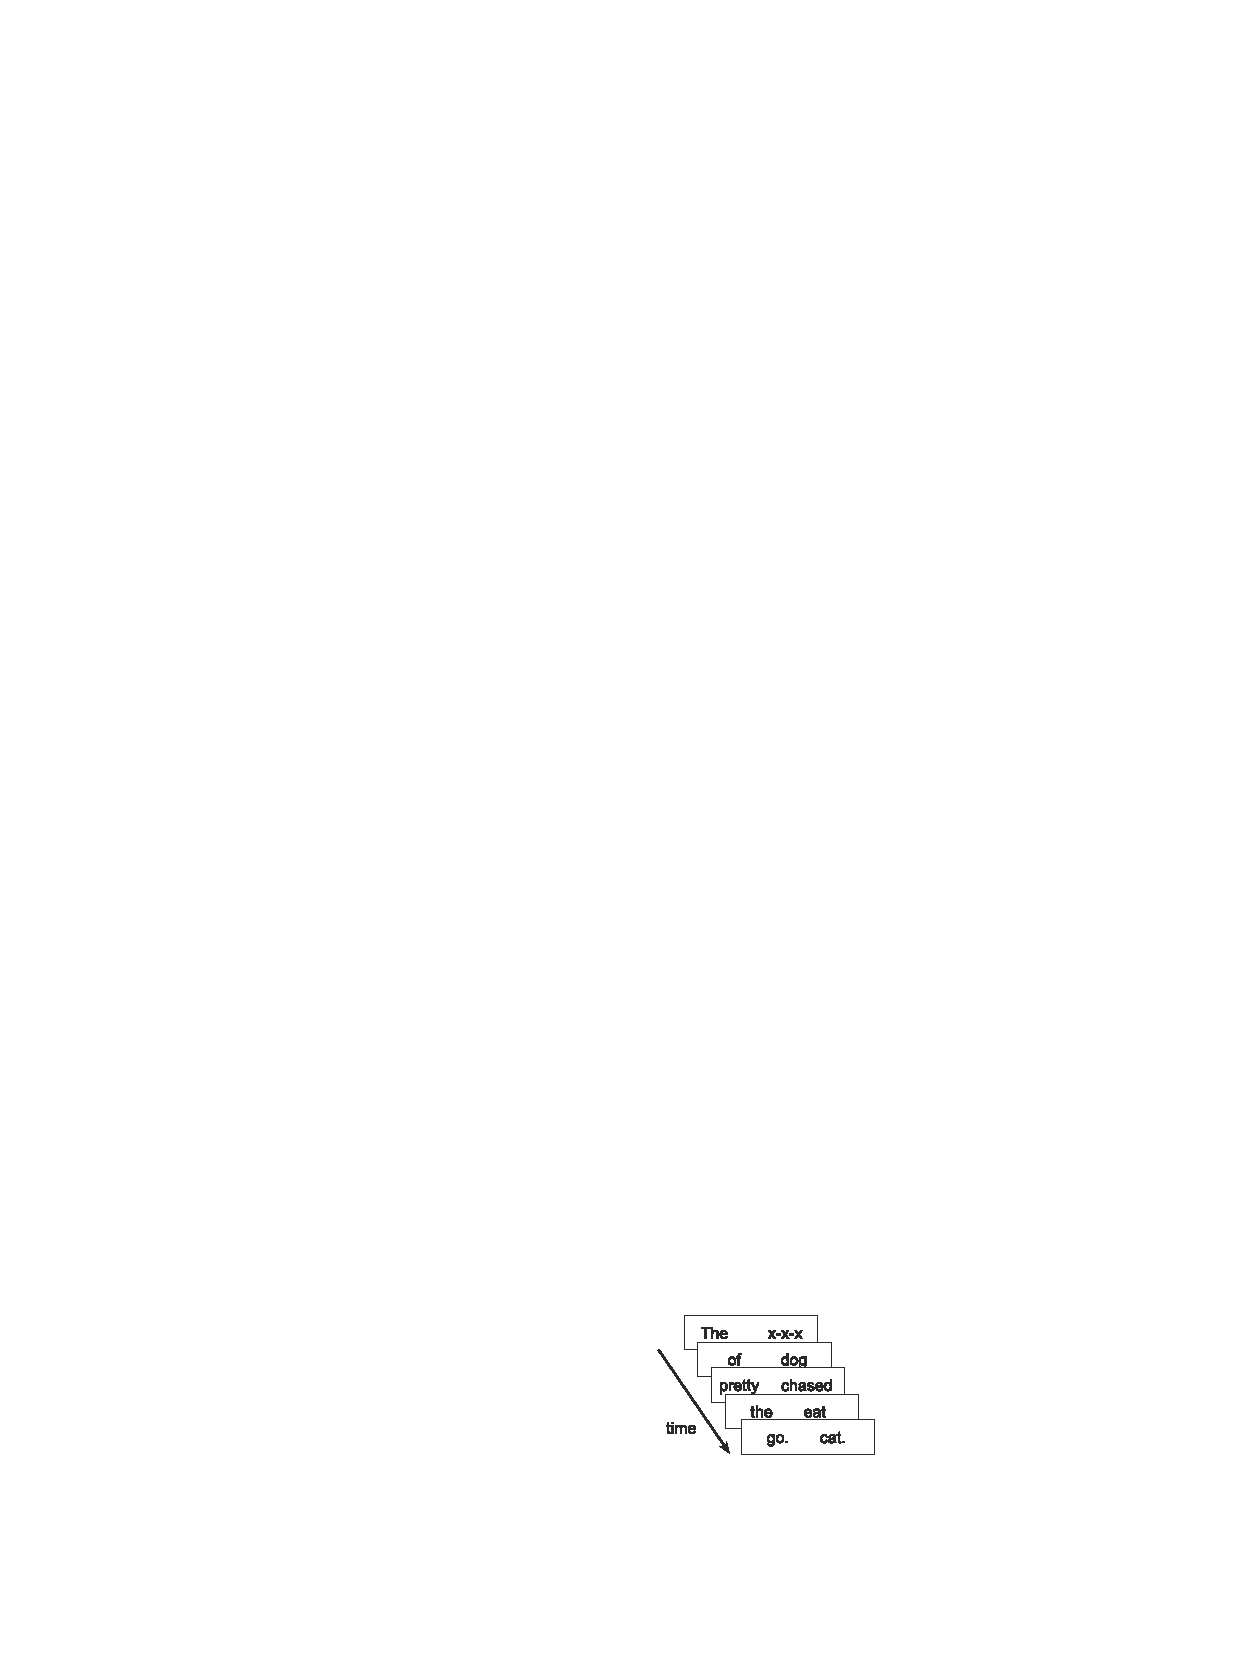
\includegraphics[width=0.5\linewidth,height=\textheight,keepaspectratio]{Chapters/Compound Nouns/Figures/mazevisualization.pdf}

}

\end{figure}%

Sentences were presented in a random order and each word was presented
an equal number of times on the left and right side of the screen.
Additionally, each item appeared an equal number of times in the
implausible and plausible context and no participant was presented with
the same item in more than one condition. The complete dataset included
9994 response tokens.

\subsubsection{Analysis}\label{analysis}

The data was analyzed using Bayesian linear regression models, as
implemented in the \emph{brms} package
(\citeproc{ref-burknerBrmsPackageBayesian2017}{Bürkner, 2017}) within
the R programming environment R Core Team
(\citeproc{ref-Rpackage}{2022}). We subsetted the data into two sets
based on the region: one set for the first noun in the compound noun and
one set for the second noun in the compound. The primary dependent
variable was log reaction time for both of these regions (following
\citeproc{ref-boyceMazeMadeEasy2020}{Boyce et al., 2020}). The primary
independent variables were plausibility and familiarity (following
\citeproc{ref-staubTimeCoursePlausibility2007}{Staub et al., 2007}). We
modeled reaction time as a function of plausibility and familiarity,
including their interaction, with maximal random effects
(\citeproc{ref-barrRandomEffectsStructure2013}{Barr et al., 2013}). The
formula used for the model is presented in equation
Equation~\ref{eq-modelfamil} below, with \emph{Plaus} as plausibility
and \emph{Famil} as familiarity. All models were sum-coded
\begin{equation}\phantomsection\label{eq-modelfamil}{
Reaction Time \sim Plaus*Famil+(Plaus*Famil|Subject)+(Plaus|Item)
}\end{equation}

\subsection{Results}\label{results}

As mentioned in the methods section, for the purpose of the analysis,
the data was divided into two regions: the N1 region and the N2 region,
which were the first and second noun in the compound noun respectively.
The results of the Bayesian regression model for the N1 region are
presented in Table~\ref{tbl-N1Staub} and in Figure~\ref{fig-N1Staub},
and the results of the N2 region are presented in
Table~\ref{tbl-N2Staub} and in Figure~\ref{fig-N2Staub}.

For the N1 region, there was an increase in reaction time for the
implausible condition relative to the plausible condition. There was no
such effect for familiarity. In other words, while participants took
longer selecting the correct word in the implausible condition, their
reaction times were not affected by the familiarity of the compound
noun. This is expected given that the familiarity condition was not the
frequency of the first noun, but rather the frequency of the compound
noun as a whole. Additionally, there was no interaction effect between
plausibility and familiarity.

At the N2 region, there was an increase in reaction time in the
plausible condition and a decrease in reaction time in the familiar
condition, but no interaction effect. In other words, participants were
slower to choose the correct word in the plausible condition. They were
also quicker to choose the correct word if the compound noun was
familiar. However, plausibility did not mediate the effects of
familiarity. That is to say, the size of the plausibility effect was not
different for familiar versus novel compound nouns. Following
Wagenmakers et al.
(\citeproc{ref-wagenmakers2010bayesianhypothesistesting}{2010}), a
post-hoc Bayes factor analysis was conducted to compare the interaction
effect to the null hypothesis (interaction effect = 0). We found a Bayes
Factor value of 18.15 which constitutes strong support for the null
hypothesis.

\begin{longtable}[]{@{}
  >{\raggedright\arraybackslash}p{(\linewidth - 10\tabcolsep) * \real{0.3521}}
  >{\raggedright\arraybackslash}p{(\linewidth - 10\tabcolsep) * \real{0.1268}}
  >{\raggedright\arraybackslash}p{(\linewidth - 10\tabcolsep) * \real{0.1408}}
  >{\raggedright\arraybackslash}p{(\linewidth - 10\tabcolsep) * \real{0.0986}}
  >{\raggedright\arraybackslash}p{(\linewidth - 10\tabcolsep) * \real{0.0845}}
  >{\raggedleft\arraybackslash}p{(\linewidth - 10\tabcolsep) * \real{0.1972}}@{}}

\caption{\label{tbl-N1Staub}Model results examining the effect of
plausibility and frequency for the N1 region.}

\tabularnewline

\toprule\noalign{}
\begin{minipage}[b]{\linewidth}\raggedright
\end{minipage} & \begin{minipage}[b]{\linewidth}\raggedright
Estimate
\end{minipage} & \begin{minipage}[b]{\linewidth}\raggedright
Est.Error
\end{minipage} & \begin{minipage}[b]{\linewidth}\raggedright
Q2.5
\end{minipage} & \begin{minipage}[b]{\linewidth}\raggedright
Q97.5
\end{minipage} & \begin{minipage}[b]{\linewidth}\raggedleft
\% Samples \textgreater{} 0
\end{minipage} \\
\midrule\noalign{}
\endhead
\bottomrule\noalign{}
\endlastfoot
Intercept & 6.822 & 0.023 & 6.777 & 6.866 & 100.00 \\
Plausibility & 0.060 & 0.010 & 0.040 & 0.080 & 83.86 \\
Familiarity & 0.015 & 0.015 & -0.014 & 0.044 & 100.00 \\
Plausibility:Familiarity & -0.003 & 0.010 & -0.023 & 0.017 & 38.76 \\

\end{longtable}

\begin{longtable}[]{@{}
  >{\raggedright\arraybackslash}p{(\linewidth - 10\tabcolsep) * \real{0.3472}}
  >{\raggedright\arraybackslash}p{(\linewidth - 10\tabcolsep) * \real{0.1250}}
  >{\raggedright\arraybackslash}p{(\linewidth - 10\tabcolsep) * \real{0.1389}}
  >{\raggedright\arraybackslash}p{(\linewidth - 10\tabcolsep) * \real{0.0972}}
  >{\raggedright\arraybackslash}p{(\linewidth - 10\tabcolsep) * \real{0.0972}}
  >{\raggedleft\arraybackslash}p{(\linewidth - 10\tabcolsep) * \real{0.1944}}@{}}

\caption{\label{tbl-N2Staub}Model results examining the effect of
plausibility and frequency for the N2 region.}

\tabularnewline

\toprule\noalign{}
\begin{minipage}[b]{\linewidth}\raggedright
\end{minipage} & \begin{minipage}[b]{\linewidth}\raggedright
Estimate
\end{minipage} & \begin{minipage}[b]{\linewidth}\raggedright
Est.Error
\end{minipage} & \begin{minipage}[b]{\linewidth}\raggedright
Q2.5
\end{minipage} & \begin{minipage}[b]{\linewidth}\raggedright
Q97.5
\end{minipage} & \begin{minipage}[b]{\linewidth}\raggedleft
\% Samples \textgreater{} 0
\end{minipage} \\
\midrule\noalign{}
\endhead
\bottomrule\noalign{}
\endlastfoot
Intercept & 6.874 & 0.025 & 6.824 & 6.924 & 100.00 \\
Plausibility & -0.066 & 0.009 & -0.083 & -0.049 & 0.06 \\
Familiarity & -0.070 & 0.019 & -0.109 & -0.033 & 0.00 \\
Plausibility:Familiarity & 0.003 & 0.009 & -0.015 & 0.020 & 63.36 \\

\end{longtable}

\begin{figure}[htbp]

\caption{\label{fig-N1Staub}Plot of log reaction time at the N1 region
as a function of plausibility and familiarity.}

\centering{

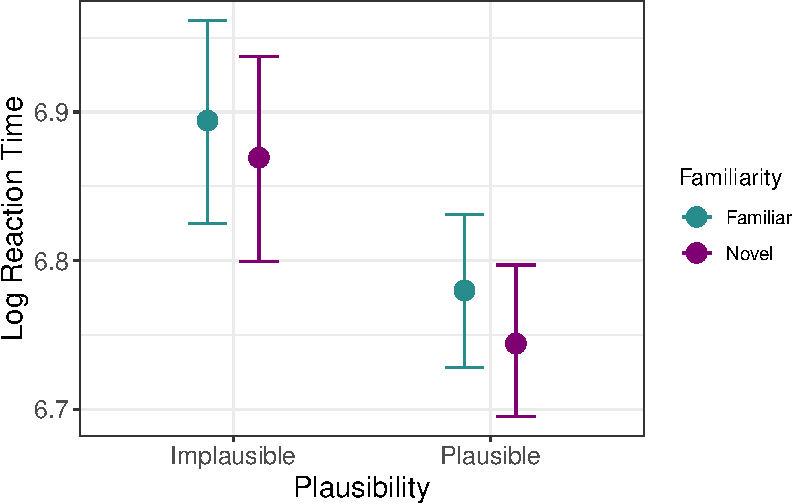
\includegraphics[width=0.8\linewidth,height=\textheight,keepaspectratio]{Chapters/Compound Nouns/staub_rep_ext_files/figure-pdf/fig-N1Staub-1.pdf}

}

\end{figure}%

\begin{figure}[htbp]

\caption{\label{fig-N2Staub}Plot of log reaction time at the N2 region
as a function of plausibility and familiarity.}

\centering{

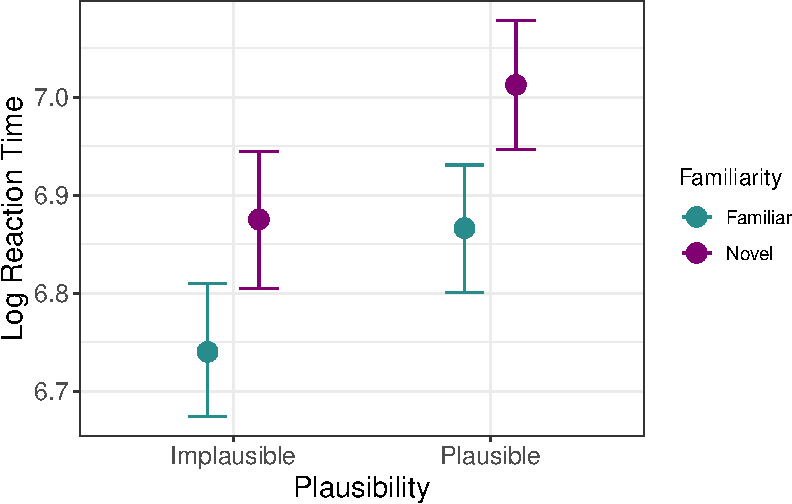
\includegraphics[width=0.8\linewidth,height=\textheight,keepaspectratio]{Chapters/Compound Nouns/staub_rep_ext_files/figure-pdf/fig-N2Staub-1.pdf}

}

\end{figure}%

\subsection{Discussion}\label{discussion}

Our results directly replicate Staub et al.
(\citeproc{ref-staubTimeCoursePlausibility2007}{2007}) using the Maze
task, demonstrating the viability of this method for the tasks at hand.
For the N1 region, while there was a clear increase in reaction time for
items in the implausible condition, there was no interaction effect
between plausibility and familiarity. In other words, the effect of
plausibility was the same for both familiar and novel compound nouns. If
familiar compound nouns are stored holistically, however, it is possible
that we would see less of a (im)plausibility effect relative to novel
items, because readers might be predicting the second noun in the
compound upon reading the first noun. Recall Table
\ref{staubsentencefamiliar}, reproduced below for convenience:

\begin{enumerate}
   \item \textbf{Novel Compound}
    \begin{enumerate}
        \item[\textbf{1a}] The zookeeper picked up the monkey medicine that was in the enclosure.
        \item[\textbf{1b}] The zookeeper spread out the monkey medicine that was in the enclosure.
    \end{enumerate} \label{staubsentencenovel}
    \item \textbf{Familiar Compound}
    \begin{enumerate}
        \item[\textbf{2a}] Jenny looked out on the huge mountain lion pacing in its cage. \label{familiarplaus}
        \item[\textbf{2b}] Jenny heard the huge mountain lion pacing in its cage. \label{familiarimplaus}
    \end{enumerate} \label{figanext}
\end{enumerate}

It is possible that if \emph{mountain lion} was stored holistically,
then upon reading \emph{Jenny heard the huge mountain\ldots{}}, the
reader might have less difficulty with the local implausibility
(relative to a low-frequency compound noun) because they would predict
\emph{lion}, which would eliminate the implausibility (\emph{heard the
mountain lion} is not implausible). However, we do not see this.
Instead, the effect of plausibility is similar for both familiar and
novel items. One possible explanation for these results is that the
familiar phrases are not necessarily stored. Instead storage might be
driven by predictability. If this is the case then it would explain why
we do not see this effect in Staub et al.
(\citeproc{ref-staubTimeCoursePlausibility2007}{2007}) or in Experiment
1, especially since all of the items used in Staub et al.
(\citeproc{ref-staubTimeCoursePlausibility2007}{2007}) are low
predictability compound nouns.

At the N2 region, the decrease in reaction time for familiarity is not
surprising given that familiarity, as previously mentioned, was based on
the frequency of the compound noun as a whole, however the increase in
reaction time for the plausible condition is interesting, especially
since the sentences were only locally implausible on the N1 region: the
second noun in the compound always eliminated the local implausibility.
It is possible this increase in reaction time is a garden path effect
for committing to an interpretation of the sentence with the N1 and
having to reanalyze the sentence. For example, when reading \emph{Jenny
looked upon the huge mountain\ldots{}}, after reading \emph{lion}, the
reader may need to reanalyze the sentence, as the subject is not looking
upon a mountain at all, but rather they are looking at a \emph{mountain
lion}. However, in the implausible condition participants may not fully
commit to the interpretation since it is locally implausible, and thus
may be waiting for a choice that eliminates the implausibility, thus
explaining the absence of a similar slowdown in the implausible
condition.

In Experiment 3, we examine whether readers can overcome this local
implausibility for high-predictability items.

\section{Experiment 2}\label{experiment-2}

\subsection{Methods}\label{methods-1}

\subsubsection{Participants}\label{participants-1}

Participant recruitment was identical to Experiment 1. 105 participants
were recruited, and 19 participants were excluded for being below 70\%
accuracy, leaving a total of 86 participants. All participants
self-reported being native English speakers.

\subsubsection{Stimuli}\label{stimuli-1}

We operationalized predictability through the odds ratio of the compound
noun to the first word when that word is not followed by the second word
in the compound noun which is exemplified in
Equation~\ref{eq-oddsratio}.

\begin{equation}\phantomsection\label{eq-oddsratio}{
\frac{\mathrm{count(\textit{peanut butter})}}{\mathrm{count(\textit{peanut})} - \mathrm{count(\textit{peanut butter})}} 
}\end{equation}

In non-mathematical terms, Equation~\ref{eq-oddsratio} quantifies how
predictable the first noun is of the second noun (i.e., how likely the
second noun is to follow after the first noun, relative to every other
word that could follow). For example, the odds ratio of \emph{peanut
butter} would be the odds ratio of the compound noun -- \emph{peanut
butter} -- to the first noun -- \emph{peanut} -- when \emph{butter} does
not follow it.

In order to collect the most predictable compound nouns, we searched the
Google \emph{n}-grams corpus
(\citeproc{ref-michel2011quantitativeanalysisculture}{Michel et al.,
2011}) using the ZS Python package
(\citeproc{ref-smithZSFileFormat2014}{Smith, 2014}). We then collected
the compound nouns with the highest predictability values, using the
following exclusion criteria: excluding words with a match count below
90,000,\footnote{This was done in order to help filter out nonsense
  words (e.g., \emph{teawhit head}) as well as eliminate words that had
  high predictability scores but were just a product of the corpus and
  unlikely to reflect the input of human learners (e.g.,
  \emph{broomwheat tea} which has a predictability score of 287 in the
  corpus).} excluding nonsense words, proper nouns, technical words
(e.g., \emph{tenth circuit}), and words in which we could not create
locally plausible and implausible sentences.\footnote{Given our
  methodology, we needed to be able to make sentences that were
  plausible and implausible using the same compound noun. This
  restriction meant we had to exclude words like \emph{Parmesan cheese}
  where it would be impossible for the reading at the N1 region to be
  implausible without the reading of the compound noun also being
  implausible.} We gathered a total of 37 compound nouns for our high
predictability condition. We subsequently normed the sentences we
created using the high predictability compounds, as well as the
sentences from Staub et al.
(\citeproc{ref-staubTimeCoursePlausibility2007}{2007}) which we
confirmed were all low predictability compounds relative to our compound
nouns.

We followed the same methodology as Staub et al.
(\citeproc{ref-staubTimeCoursePlausibility2007}{2007}) for our norming
procedure: we provided participants with each item in four conditions
(see below) and asked participants to rate each sentence on a 7-point
Likert scale in terms of how well the last word fit in the sentence. No
participant rated more than one version of each sentence.

\begin{enumerate} \setcounter{enumi}{2}
   \item \textbf{Norming Conditions}
    \begin{enumerate}
        \item[\textbf{3a}] Jimmy picked up the peanut (plausible, through the first noun).
        \item[\textbf{3b}] Jimmy picked up the peanut butter (plausible, through the second noun).
        \item[\textbf{3c}] Jimmy spread out the peanut (implausible, through the first noun).
        \item[\textbf{3d}] Jimmy spread out the peanut butter (implausible, through the second noun).
    \end{enumerate} \label{figanext}
\end{enumerate}

Finally, we excluded items in which the implausible sentence through the
first noun was rated more or similarly well to the other conditions
(i.e., the plausible sentence through the first noun, the plausible
sentence through the second noun, and the implausible sentence through
the second noun). It is important to note that due to our experimental
design, the implausible sentence through the second noun is technically
plausible at the second noun, because the second noun eliminates the
local implausibility. Thus this condition should also receive a high
rating, despite being the implausible condition. The mean values for
each condition are as follows: plausible, through the first noun: 5.58
(sd = 0.78); plausible, through the second noun: 5.41 (sd = 0.71);
implausible, through the first noun: 3.13 (0.63); implausible, through
the second noun: 5.47 (sd = 0.82).

After norming, we selected sentences such that the difference in
plausibility values between the plausible and implausible conditions
were roughly the same for the high predictability and low predictability
conditions. This was done to avoid conflating an interaction effect
between predictability and plausibility with an item-specific effect.
That is, if the plausibility effect was smaller for high predictability
sentences relative to the low predictability sentences, then it would be
impossible to tell if the interaction effect between predictability and
plausibility is meaningful or just a product of our stimuli. The mean
plausibility difference for the low predictability items was 2.47 and
the mean plausibility difference for the high predictability items was
2.48. We confirmed that there was not a significant difference in
plausibility values through a t-test (t = 0.0446, df = 39, p = 0.52).
After accounting for this, we ended up with 21 high predictability and
21 low predictability items (which were taken from
\citeproc{ref-staubTimeCoursePlausibility2007}{Staub et al., 2007}), for
a total of 42 items. Lastly, in order to avoid participants discerning
the experimental design we also included 188 filler items.

\subsubsection{Procedure}\label{procedure-1}

Following Experiment 1, we used the A-maze task
(\citeproc{ref-boyceMazeMadeEasy2020}{Boyce et al., 2020}) with
automatically-generated distractor items
(\citeproc{ref-gulordava2018colorlessgreenrecurrent}{Gulordava et al.,
n.d.}). Our dependent variable was reaction time and our independent
variables were plausibility and predictability. We again used ibex farm
to run our maze task. Sentences were presented in a random order and
each word was presented an equal amount of times on the left and right
side of the screen. Additionally, each item appeared an equal number of
times in the implausible and plausible context and no participant was
presented with the same item in more than one condition.

\subsubsection{Analysis}\label{analysis-1}

The data was analyzed using Bayesian linear regression models, as
implemented in the \emph{brms} package
(\citeproc{ref-burknerBrmsPackageBayesian2017}{Bürkner, 2017}) within
the R programming environment (\citeproc{ref-Rpackage}{R Core Team,
2022}). We subsetted the data into two sets based on the region: one set
for the first noun in the compound noun and one set for the second noun
in the compound. The primary dependent variable was log reaction time
for both of these regions (following
\citeproc{ref-boyceMazeMadeEasy2020}{Boyce et al., 2020}). The
independent variables were plausibility and predictability. Reaction
time was modeled as a function of plausibility and predictability, along
with their interaction, with maximal random effects
(\citeproc{ref-barrRandomEffectsStructure2013}{Barr et al., 2013}). The
formula used for the model is presented in Equation~\ref{eq-model2}
below, with \emph{Plaus} as plausibility and \emph{Predic} as
predictability.

\begin{equation}\phantomsection\label{eq-model2}{
Reaction Time\sim Plaus*Predict+(Plaus*Predict|Subject)+(Plaus|Item) 
}\end{equation}

\subsection{Results}\label{results-1}

As mentioned in the methods section, for the purpose of the analysis,
the data was divided into two regions: the N1 region and the N2 region,
which were the first and second noun in the compound noun respectively.
The results of the Bayesian regression models for the N1 region are
presented in Table~\ref{tbl-N1Predictability} and
Table~\ref{tbl-N1LogOdds}, and visualized in
Figure~\ref{fig-N1Predictability} and Figure~\ref{fig-N1LogOdds}. The
results of the N2 region are presented in
Table~\ref{tbl-N2Predictability} and Table~\ref{tbl-N2LogOdds}, and
visualized in Figure~\ref{fig-N2Predictability} and
Figure~\ref{fig-N2LogOdds}.

With regards to the N1 region, Table~\ref{tbl-N1Predictability} presents
the results of the analysis we ran with predictability as a binary
predictor (high or low), while Table~\ref{tbl-N1LogOdds} presents the
results of the analysis we ran with predictability as a continuous
predictor (operationalized as the log odds ratio). Our results
demonstrate that, similar to experiment 1, there was an increase in
reaction time for the implausible condition, but no effect for
predictability or the interaction between the two.

With regards to the N2 region, Table~\ref{tbl-N2Predictability} presents
the results of the analysis we ran with predictability as a binary
predictor (high or low), while Table~\ref{tbl-N2LogOdds} presents the
results of the analysis we ran with predictability as a continuous
predictor (operationalized as the log odds ratio). Our results, as in
Experiment 1, demonstrate an increase in reaction time in the plausible
condition and and a decrease in reaction time in the high-predictability
condition, but no interaction effect between plausibility and
predictability. As in Experiment 1, we once again conducted a post-hoc
Bayes factor analysis to compare the interaction effect to the null
hypothesis (interaction effect = 0). We found a Bayes Factor value of
15.67 which constitutes strong support for the null hypothesis.

Figure~\ref{fig-N1Predictability} and Figure~\ref{fig-N2Predictability}
provide visualizations of the analyses run with predictability as a
binary variable while Figure~\ref{fig-N1LogOdds} and
Figure~\ref{fig-N2LogOdds} present analyses with predictability as a
continuous variable.

\begin{longtable}[]{@{}
  >{\raggedright\arraybackslash}p{(\linewidth - 10\tabcolsep) * \real{0.3784}}
  >{\raggedright\arraybackslash}p{(\linewidth - 10\tabcolsep) * \real{0.1216}}
  >{\raggedright\arraybackslash}p{(\linewidth - 10\tabcolsep) * \real{0.1351}}
  >{\raggedright\arraybackslash}p{(\linewidth - 10\tabcolsep) * \real{0.0946}}
  >{\raggedright\arraybackslash}p{(\linewidth - 10\tabcolsep) * \real{0.0811}}
  >{\raggedleft\arraybackslash}p{(\linewidth - 10\tabcolsep) * \real{0.1892}}@{}}

\caption{\label{tbl-N1Predictability}Regression analysis results for the
N1 region with predictability as a binary predictor (high or low).}

\tabularnewline

\toprule\noalign{}
\begin{minipage}[b]{\linewidth}\raggedright
\end{minipage} & \begin{minipage}[b]{\linewidth}\raggedright
Estimate
\end{minipage} & \begin{minipage}[b]{\linewidth}\raggedright
Est.Error
\end{minipage} & \begin{minipage}[b]{\linewidth}\raggedright
Q2.5
\end{minipage} & \begin{minipage}[b]{\linewidth}\raggedright
Q97.5
\end{minipage} & \begin{minipage}[b]{\linewidth}\raggedleft
\% Samples \textgreater{} 0
\end{minipage} \\
\midrule\noalign{}
\endhead
\bottomrule\noalign{}
\endlastfoot
Intercept & 6.879 & 0.029 & 6.823 & 6.936 & 100.00 \\
Plausibility & 0.068 & 0.014 & 0.041 & 0.095 & 100.00 \\
Predictability & 0.034 & 0.024 & -0.012 & 0.081 & 92.30 \\
Plausibility:Predictability & -0.001 & 0.013 & -0.027 & 0.025 & 46.72 \\

\end{longtable}

\begin{longtable}[]{@{}
  >{\raggedright\arraybackslash}p{(\linewidth - 10\tabcolsep) * \real{0.3134}}
  >{\raggedright\arraybackslash}p{(\linewidth - 10\tabcolsep) * \real{0.1343}}
  >{\raggedright\arraybackslash}p{(\linewidth - 10\tabcolsep) * \real{0.1493}}
  >{\raggedright\arraybackslash}p{(\linewidth - 10\tabcolsep) * \real{0.1045}}
  >{\raggedright\arraybackslash}p{(\linewidth - 10\tabcolsep) * \real{0.0896}}
  >{\raggedleft\arraybackslash}p{(\linewidth - 10\tabcolsep) * \real{0.2090}}@{}}

\caption{\label{tbl-N1LogOdds}Regression analysis results for the N1
region with predictability as a continuous predictor (log odds ratio).}

\tabularnewline

\toprule\noalign{}
\begin{minipage}[b]{\linewidth}\raggedright
\end{minipage} & \begin{minipage}[b]{\linewidth}\raggedright
Estimate
\end{minipage} & \begin{minipage}[b]{\linewidth}\raggedright
Est.Error
\end{minipage} & \begin{minipage}[b]{\linewidth}\raggedright
Q2.5
\end{minipage} & \begin{minipage}[b]{\linewidth}\raggedright
Q97.5
\end{minipage} & \begin{minipage}[b]{\linewidth}\raggedleft
\% Samples \textgreater{} 0
\end{minipage} \\
\midrule\noalign{}
\endhead
\bottomrule\noalign{}
\endlastfoot
Intercept & 6.876 & 0.030 & 6.817 & 6.935 & 100.00 \\
Plausibility & 0.069 & 0.013 & 0.042 & 0.095 & 100.00 \\
LogOdds & 0.005 & 0.007 & -0.009 & 0.020 & 76.50 \\
Plausibility:LogOdds & 0.001 & 0.004 & -0.007 & 0.009 & 61.64 \\

\end{longtable}

\begin{longtable}[]{@{}
  >{\raggedright\arraybackslash}p{(\linewidth - 10\tabcolsep) * \real{0.3733}}
  >{\raggedright\arraybackslash}p{(\linewidth - 10\tabcolsep) * \real{0.1200}}
  >{\raggedright\arraybackslash}p{(\linewidth - 10\tabcolsep) * \real{0.1333}}
  >{\raggedright\arraybackslash}p{(\linewidth - 10\tabcolsep) * \real{0.0933}}
  >{\raggedright\arraybackslash}p{(\linewidth - 10\tabcolsep) * \real{0.0933}}
  >{\raggedleft\arraybackslash}p{(\linewidth - 10\tabcolsep) * \real{0.1867}}@{}}

\caption{\label{tbl-N2Predictability}Regression analysis results for the
N2 region with predictability as a binary predictor (high or low).}

\tabularnewline

\toprule\noalign{}
\begin{minipage}[b]{\linewidth}\raggedright
\end{minipage} & \begin{minipage}[b]{\linewidth}\raggedright
Estimate
\end{minipage} & \begin{minipage}[b]{\linewidth}\raggedright
Est.Error
\end{minipage} & \begin{minipage}[b]{\linewidth}\raggedright
Q2.5
\end{minipage} & \begin{minipage}[b]{\linewidth}\raggedright
Q97.5
\end{minipage} & \begin{minipage}[b]{\linewidth}\raggedleft
\% Samples \textgreater{} 0
\end{minipage} \\
\midrule\noalign{}
\endhead
\bottomrule\noalign{}
\endlastfoot
Intercept & 6.793 & 0.029 & 6.738 & 6.852 & 100.00 \\
Plausibility & -0.072 & 0.012 & -0.097 & -0.049 & 0.00 \\
Predictability & -0.080 & 0.026 & -0.132 & -0.030 & 0.12 \\
Plausibility:Predictability & 0.005 & 0.012 & -0.017 & 0.028 & 67.46 \\

\end{longtable}

\begin{longtable}[]{@{}
  >{\raggedright\arraybackslash}p{(\linewidth - 10\tabcolsep) * \real{0.3088}}
  >{\raggedright\arraybackslash}p{(\linewidth - 10\tabcolsep) * \real{0.1324}}
  >{\raggedright\arraybackslash}p{(\linewidth - 10\tabcolsep) * \real{0.1471}}
  >{\raggedright\arraybackslash}p{(\linewidth - 10\tabcolsep) * \real{0.1029}}
  >{\raggedright\arraybackslash}p{(\linewidth - 10\tabcolsep) * \real{0.1029}}
  >{\raggedleft\arraybackslash}p{(\linewidth - 10\tabcolsep) * \real{0.2059}}@{}}

\caption{\label{tbl-N2LogOdds}Regression analysis results for the N2
region with predictability as a continuous predictor (log odds ratio).}

\tabularnewline

\toprule\noalign{}
\begin{minipage}[b]{\linewidth}\raggedright
\end{minipage} & \begin{minipage}[b]{\linewidth}\raggedright
Estimate
\end{minipage} & \begin{minipage}[b]{\linewidth}\raggedright
Est.Error
\end{minipage} & \begin{minipage}[b]{\linewidth}\raggedright
Q2.5
\end{minipage} & \begin{minipage}[b]{\linewidth}\raggedright
Q97.5
\end{minipage} & \begin{minipage}[b]{\linewidth}\raggedleft
\% Samples \textgreater{} 0
\end{minipage} \\
\midrule\noalign{}
\endhead
\bottomrule\noalign{}
\endlastfoot
Intercept & 6.802 & 0.026 & 6.752 & 6.853 & 100.00 \\
Plausibility & -0.073 & 0.012 & -0.097 & -0.048 & 0.00 \\
LogOdds & -0.033 & 0.007 & -0.046 & -0.019 & 0.00 \\
Plausibility:LogOdds & 0.001 & 0.004 & -0.006 & 0.008 & 60.44 \\

\end{longtable}

\begin{figure}[htbp]

\caption{\label{fig-N1Predictability}Plot of the N1 region with
predictability as a binary variable (high or low).}

\centering{

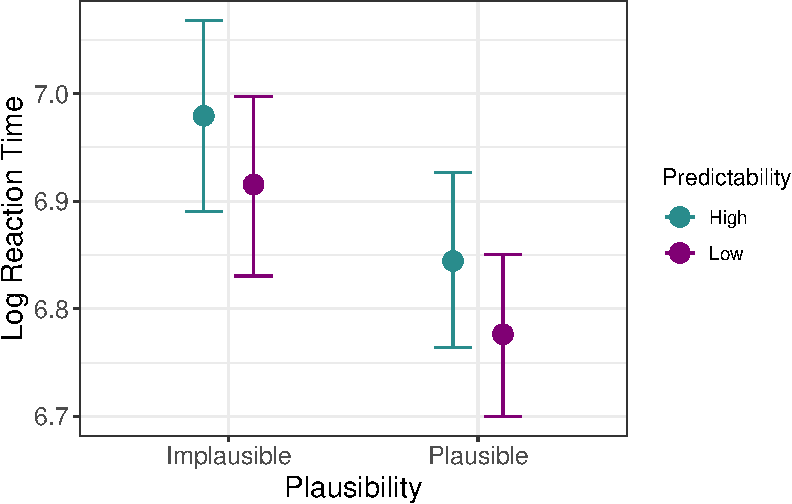
\includegraphics[width=0.8\linewidth,height=\textheight,keepaspectratio]{Chapters/Compound Nouns/staub_rep_ext_files/figure-pdf/fig-N1Predictability-1.pdf}

}

\end{figure}%

\begin{figure}[htbp]

\caption{\label{fig-N1LogOdds}Plot of the N1 region with predictability
as a continuous variable.}

\centering{

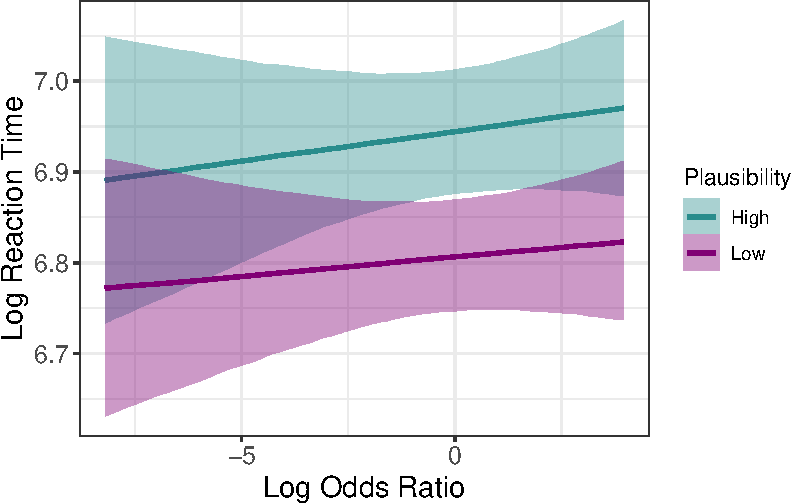
\includegraphics[width=0.8\linewidth,height=\textheight,keepaspectratio]{Chapters/Compound Nouns/staub_rep_ext_files/figure-pdf/fig-N1LogOdds-1.pdf}

}

\end{figure}%

\begin{figure}[htbp]

\caption{\label{fig-N2Predictability}Plot of the N2 region with
predictability as a binary variable (high or low).}

\centering{

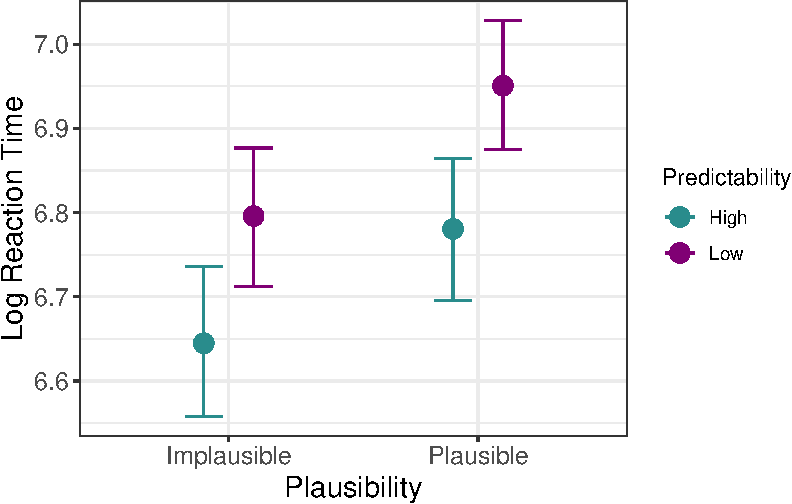
\includegraphics[width=0.8\linewidth,height=\textheight,keepaspectratio]{Chapters/Compound Nouns/staub_rep_ext_files/figure-pdf/fig-N2Predictability-1.pdf}

}

\end{figure}%

\begin{figure}[htbp]

\caption{\label{fig-N2LogOdds}Plot of the N2 region with predictability
as a continuous variable.}

\centering{

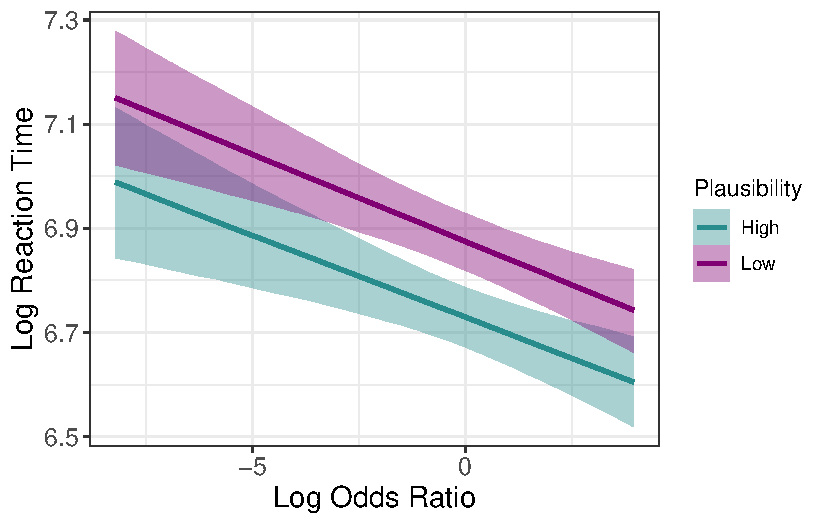
\includegraphics[width=0.8\linewidth,height=\textheight,keepaspectratio]{Chapters/Compound Nouns/staub_rep_ext_files/figure-pdf/fig-N2LogOdds-1.pdf}

}

\end{figure}%

\subsection{Discussion}\label{discussion-1}

Experiment 2 replicates and extends Experiment 1 using predictability
instead of familiarity (i.e., phrasal frequency). Interestingly, the
results of Experiment 2 were extremely similar to the results of
Experiment 1: There was no interaction effect between predictability and
plausibility on the RTs for the N1 condition. Additionally, while we see
an effect of implausibility on the N1 region, we don't see an effect of
predictability. This is expected since predictability is defined as the
odds that the N2 appears given the N1, so we should see this effect on
the N2 region, not the N1 region.

The results of the N2 region also bear remarkable similarities to our
results in Experiment 1: There was a plausibility and predictability
effect, but no interaction between the two. Specifically, there was an
\emph{increase} in reaction time for items in the plausible condition
relative to the implausible condition. It is possible that, as mentioned
in the discussion section of Experiment 1, this increase in reaction
time is a garden path effect for committing to an interpretation of the
sentence with the N1 and having to reanalyze the sentence.

\section{Experiment 3}\label{experiment-3}

In Experiment 3, we directly replicate Experiment 1 using eye-tracking.

\subsection{Methods}\label{methods-2}

\subsubsection{Participants}\label{participants-2}

46 native English speakers were recruited from the University of
California, Davis subjects pool. They were given course credit in
exchange for their participation. All participants had normal or
corrected vision.

\subsubsection{Materials}\label{materials}

The materials were identical to Experiment 1.

We recorded participants' eye movements using the Eyelink 1000 Plus. We
recorded pupil movements from the right eye. Participants were seated
850mm away from the screen. Our screen resolution was 1920x1080, 531.3mm
in width, and 298.8mm in height.

Comprehension was checked for non-experimental trials and participants
below 80\% accuracy were excluded. Out of our 56 participants, 0 were
excluded for falling below the accuracy threshold.

\subsubsection{Analyses}\label{analyses}

Prior to our analyses, sentences with blinks were excluded and fixations
less than 80ms in duration and within one character of the nearest
fixation were merged into that fixation (following
\citeproc{ref-staubTimeCoursePlausibility2007}{Staub et al., 2007}). For
our regions of interest (the first noun and the second noun in the
compound noun), we computed first fixation duration, first pass time,
go-past time, and first-pass regression.

For each analysis, our independent variables were plausibility (high or
low) and familiarity (high or low) and their interaction. We also
included random slopes for condition and predictability by subject and
plausibility by compound noun as well as intercepts for subject and
compound noun. For each of our models, we used sum-coding, where the
intercept represents the grand mean and the fixed-effect coefficient
estimates represent the distance from the grand mean.

\subsection{Results}\label{results-2}

\subsubsection{First Fixation Times}\label{first-fixation-times}

\paragraph{N1}\label{n1}

Our results for the effects of plausibility and familiarity on first
fixation times are described in Table~\ref{tbl-firstfixn1staub} and
visualized in Figure~\ref{fig-firstfixn1staub}.

We find an effect of plausibility, however we find no effect for
familiarity and no interaction effect. The results suggest that
regardless of familiarity, participants' first fixations are longer in
the implausible context.

\begin{longtable}[]{@{}
  >{\raggedright\arraybackslash}p{(\linewidth - 10\tabcolsep) * \real{0.3378}}
  >{\raggedright\arraybackslash}p{(\linewidth - 10\tabcolsep) * \real{0.1216}}
  >{\raggedright\arraybackslash}p{(\linewidth - 10\tabcolsep) * \real{0.1351}}
  >{\raggedright\arraybackslash}p{(\linewidth - 10\tabcolsep) * \real{0.1081}}
  >{\raggedright\arraybackslash}p{(\linewidth - 10\tabcolsep) * \real{0.1081}}
  >{\raggedleft\arraybackslash}p{(\linewidth - 10\tabcolsep) * \real{0.1892}}@{}}

\caption{\label{tbl-firstfixn1staub}Model results examining the effect
of plausibility and frequency on first fixation times for the N1
region.}

\tabularnewline

\toprule\noalign{}
\begin{minipage}[b]{\linewidth}\raggedright
\end{minipage} & \begin{minipage}[b]{\linewidth}\raggedright
Estimate
\end{minipage} & \begin{minipage}[b]{\linewidth}\raggedright
Est.Error
\end{minipage} & \begin{minipage}[b]{\linewidth}\raggedright
Q2.5
\end{minipage} & \begin{minipage}[b]{\linewidth}\raggedright
Q97.5
\end{minipage} & \begin{minipage}[b]{\linewidth}\raggedleft
\% Samples \textgreater{} 0
\end{minipage} \\
\midrule\noalign{}
\endhead
\bottomrule\noalign{}
\endlastfoot
Intercept & 239.234 & 5.536 & 228.463 & 250.049 & 100.000 \\
Plausibility & 4.188 & 2.156 & -0.022 & 8.378 & 97.400 \\
Familiarity & -0.866 & 2.399 & -5.589 & 3.784 & 35.525 \\
Plausibility:Familiarity & 0.027 & 2.398 & -4.843 & 4.782 & 49.675 \\

\end{longtable}

\begin{figure}[htbp]

\caption{\label{fig-firstfixn1staub}Visualization of the effects of
plausibility and familiarity on first fixation times for the N1 region.}

\centering{

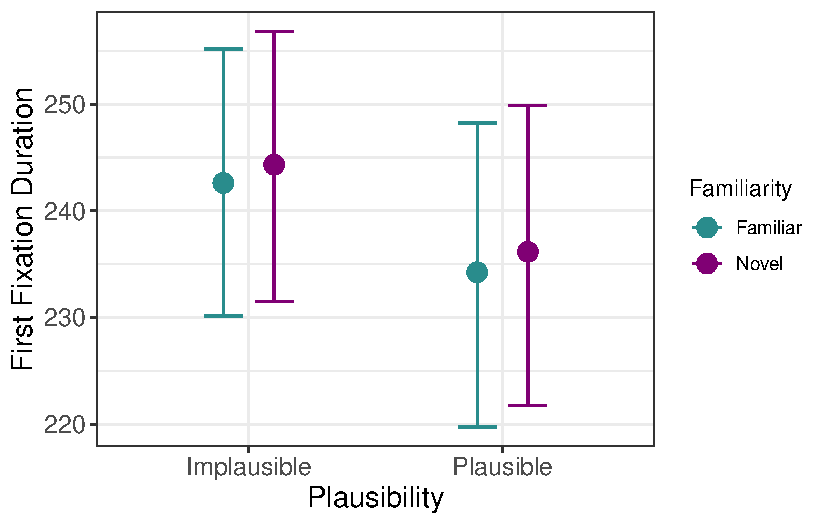
\includegraphics[width=0.8\linewidth,height=\textheight,keepaspectratio]{Chapters/Compound Nouns/staub_rep_ext_files/figure-pdf/fig-firstfixn1staub-1.pdf}

}

\end{figure}%

\paragraph{N2}\label{n2}

Our results for the effects of plausibility and familiarity on first
fixation times on the N2 region are described in
Table~\ref{tbl-firstfixn2staub} and visualized in
Figure~\ref{fig-firstfixn2staub}.

We find an effect of plausibility, however we find no effect for
familiarity and no interaction effect. The results suggest that
regardless of familiarity, participants' first fixations are longer in
the implausible context.

Our results suggest an effect of familiarity such that familiar items
had shorter first fixation times. We find no effect of plausibility
which is expected because the N2 has no difference in terms of
plausibility. We also find no interaction effect. These results suggest
that readers' first fixation times on the N2 region are shorter for the
familiar compounds.

\begin{longtable}[]{@{}
  >{\raggedright\arraybackslash}p{(\linewidth - 10\tabcolsep) * \real{0.3378}}
  >{\raggedright\arraybackslash}p{(\linewidth - 10\tabcolsep) * \real{0.1216}}
  >{\raggedright\arraybackslash}p{(\linewidth - 10\tabcolsep) * \real{0.1351}}
  >{\raggedright\arraybackslash}p{(\linewidth - 10\tabcolsep) * \real{0.1081}}
  >{\raggedright\arraybackslash}p{(\linewidth - 10\tabcolsep) * \real{0.1081}}
  >{\raggedleft\arraybackslash}p{(\linewidth - 10\tabcolsep) * \real{0.1892}}@{}}

\caption{\label{tbl-firstfixn2staub}Model results examining the effect
of plausibility and familiarity on first fixation times for the N2
region.}

\tabularnewline

\toprule\noalign{}
\begin{minipage}[b]{\linewidth}\raggedright
\end{minipage} & \begin{minipage}[b]{\linewidth}\raggedright
Estimate
\end{minipage} & \begin{minipage}[b]{\linewidth}\raggedright
Est.Error
\end{minipage} & \begin{minipage}[b]{\linewidth}\raggedright
Q2.5
\end{minipage} & \begin{minipage}[b]{\linewidth}\raggedright
Q97.5
\end{minipage} & \begin{minipage}[b]{\linewidth}\raggedleft
\% Samples \textgreater{} 0
\end{minipage} \\
\midrule\noalign{}
\endhead
\bottomrule\noalign{}
\endlastfoot
Intercept & 249.615 & 6.468 & 236.382 & 262.346 & 100.000 \\
Plausibility & -2.094 & 2.652 & -7.400 & 3.120 & 21.575 \\
Familiarity & -6.973 & 4.270 & -15.430 & 1.443 & 5.425 \\
Plausibility:Familiarity & -1.055 & 2.365 & -5.669 & 3.620 & 32.475 \\

\end{longtable}

\begin{figure}[htbp]

\caption{\label{fig-firstfixn2staub}Visualization of the effects of
plausibility and familiarity on first fixation times for the N2 region.}

\centering{

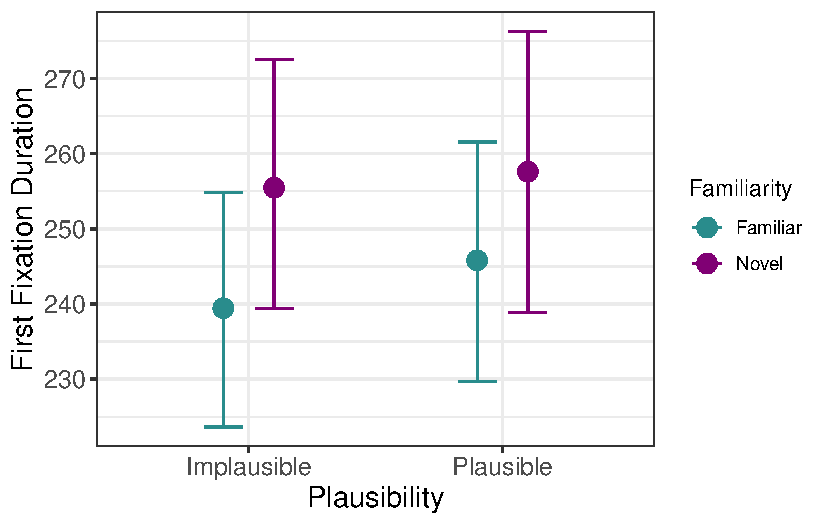
\includegraphics[width=0.8\linewidth,height=\textheight,keepaspectratio]{Chapters/Compound Nouns/staub_rep_ext_files/figure-pdf/fig-firstfixn2staub-1.pdf}

}

\end{figure}%

\subsubsection{Gaze/First-Pass Time}\label{gazefirst-pass-time}

\paragraph{N1}\label{n1-1}

Our results for the effects of plausibility and familiarity on
gaze/first-pass times on the N1 region are described in
Table~\ref{tbl-gazen1staub} and visualized in
Figure~\ref{fig-gazen1staub}.

We find no effect of plausibility or familiarity on reading times for
the N1 region. These results suggest that readers' gaze/first-pass times
were not sensitive to the plausibility manipulation.

\begin{longtable}[]{@{}
  >{\raggedright\arraybackslash}p{(\linewidth - 10\tabcolsep) * \real{0.3378}}
  >{\raggedright\arraybackslash}p{(\linewidth - 10\tabcolsep) * \real{0.1216}}
  >{\raggedright\arraybackslash}p{(\linewidth - 10\tabcolsep) * \real{0.1351}}
  >{\raggedright\arraybackslash}p{(\linewidth - 10\tabcolsep) * \real{0.1081}}
  >{\raggedright\arraybackslash}p{(\linewidth - 10\tabcolsep) * \real{0.1081}}
  >{\raggedleft\arraybackslash}p{(\linewidth - 10\tabcolsep) * \real{0.1892}}@{}}

\caption{\label{tbl-gazen1staub}Model results examining the effect of
plausibility and familiarity on gaze/first-pass times for the N1
region.}

\tabularnewline

\toprule\noalign{}
\begin{minipage}[b]{\linewidth}\raggedright
\end{minipage} & \begin{minipage}[b]{\linewidth}\raggedright
Estimate
\end{minipage} & \begin{minipage}[b]{\linewidth}\raggedright
Est.Error
\end{minipage} & \begin{minipage}[b]{\linewidth}\raggedright
Q2.5
\end{minipage} & \begin{minipage}[b]{\linewidth}\raggedright
Q97.5
\end{minipage} & \begin{minipage}[b]{\linewidth}\raggedleft
\% Samples \textgreater{} 0
\end{minipage} \\
\midrule\noalign{}
\endhead
\bottomrule\noalign{}
\endlastfoot
Intercept & 273.963 & 8.562 & 257.093 & 290.927 & 100.000 \\
Plausibility & 0.037 & 0.195 & -0.334 & 0.422 & 57.825 \\
Familiarity & -0.003 & 0.199 & -0.399 & 0.381 & 49.725 \\
Plausibility:Familiarity & 0.009 & 0.199 & -0.376 & 0.404 & 51.925 \\

\end{longtable}

\newpage

\begin{figure}[htbp]

\caption{\label{fig-gazen1staub}Visualization of the effects of
plausibility and familiarity on Gaze/first-pass times for the N1
region.}

\centering{

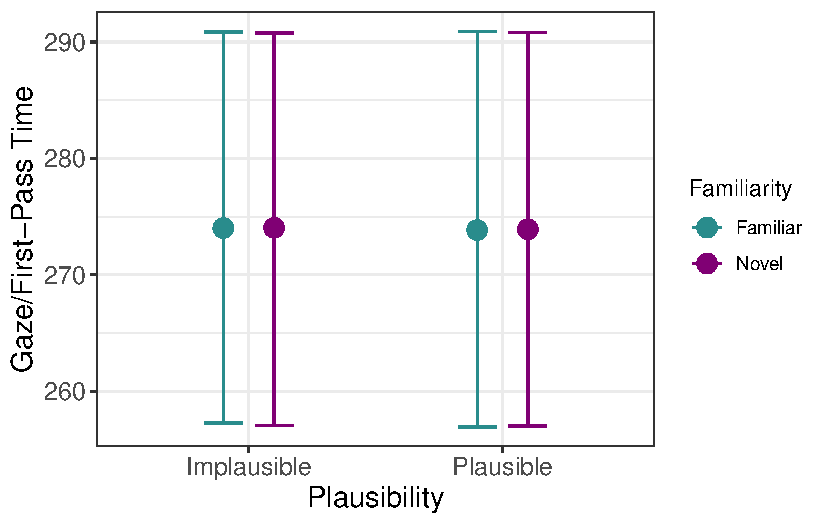
\includegraphics[width=0.8\linewidth,height=\textheight,keepaspectratio]{Chapters/Compound Nouns/staub_rep_ext_files/figure-pdf/fig-gazen1staub-1.pdf}

}

\end{figure}%

\paragraph{N2}\label{n2-1}

Our results for the effects of plausibility and familiarity on
gaze/first-pass times on the N2 region are described in
Table~\ref{tbl-gazen2staub} and visualized in
Figure~\ref{fig-gazen2staub}.

We find no effect of plausibility, but we do find an effect of
familiarity on reading times for the N2 region. These results suggest
that readers' gaze/first-pass times on the N2 region were shorter for
familiar compounds.

\begin{longtable}[]{@{}
  >{\raggedright\arraybackslash}p{(\linewidth - 10\tabcolsep) * \real{0.3378}}
  >{\raggedright\arraybackslash}p{(\linewidth - 10\tabcolsep) * \real{0.1216}}
  >{\raggedright\arraybackslash}p{(\linewidth - 10\tabcolsep) * \real{0.1351}}
  >{\raggedright\arraybackslash}p{(\linewidth - 10\tabcolsep) * \real{0.1081}}
  >{\raggedright\arraybackslash}p{(\linewidth - 10\tabcolsep) * \real{0.1081}}
  >{\raggedleft\arraybackslash}p{(\linewidth - 10\tabcolsep) * \real{0.1892}}@{}}

\caption{\label{tbl-gazen2staub}Model results examining the effect of
plausibility and familiarity on gaze/first-pass times for the N2
region.}

\tabularnewline

\toprule\noalign{}
\begin{minipage}[b]{\linewidth}\raggedright
\end{minipage} & \begin{minipage}[b]{\linewidth}\raggedright
Estimate
\end{minipage} & \begin{minipage}[b]{\linewidth}\raggedright
Est.Error
\end{minipage} & \begin{minipage}[b]{\linewidth}\raggedright
Q2.5
\end{minipage} & \begin{minipage}[b]{\linewidth}\raggedright
Q97.5
\end{minipage} & \begin{minipage}[b]{\linewidth}\raggedleft
\% Samples \textgreater{} 0
\end{minipage} \\
\midrule\noalign{}
\endhead
\bottomrule\noalign{}
\endlastfoot
Intercept & 275.485 & 9.039 & 257.696 & 293.098 & 100.0000 \\
Plausibility & 0.048 & 3.755 & -7.501 & 7.445 & 50.5500 \\
Familiarity & -12.956 & 6.366 & -24.981 & -0.202 & 2.3250 \\
Plausibility:Familiarity & -3.879 & 3.775 & -11.309 & 3.425 & 15.2375 \\

\end{longtable}

\begin{figure}[htbp]

\caption{\label{fig-gazen2staub}Visualization of the effects of
plausibility and familiarity on gaze/first-pass times for the N2
region.}

\centering{

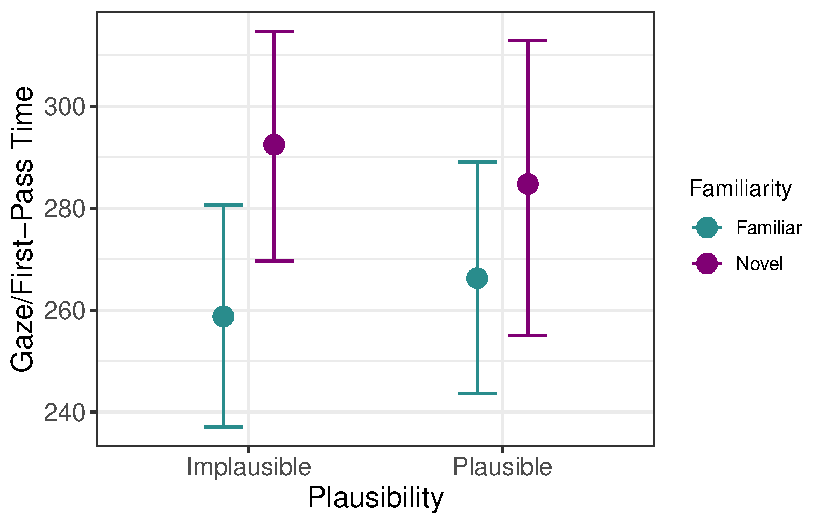
\includegraphics[width=0.8\linewidth,height=\textheight,keepaspectratio]{Chapters/Compound Nouns/staub_rep_ext_files/figure-pdf/fig-gazen2staub-1.pdf}

}

\end{figure}%

\subsubsection{Go-Past Time}\label{go-past-time}

\paragraph{N1}\label{n1-2}

Our results for the effects of plausibility and familiarity on go-past
times in the N1 region are described in Table~\ref{tbl-gopastn1staub}
and visualized in Figure~\ref{fig-gopastn1staub}.

Our results suggest a main-effect of plausibility as well as an
interaction effect between plausibility and familiarity such that the
increase in go-past times for familiar items is much greater than the
increase is for novel items.

\begin{longtable}[]{@{}
  >{\raggedright\arraybackslash}p{(\linewidth - 10\tabcolsep) * \real{0.3378}}
  >{\raggedright\arraybackslash}p{(\linewidth - 10\tabcolsep) * \real{0.1216}}
  >{\raggedright\arraybackslash}p{(\linewidth - 10\tabcolsep) * \real{0.1351}}
  >{\raggedright\arraybackslash}p{(\linewidth - 10\tabcolsep) * \real{0.1081}}
  >{\raggedright\arraybackslash}p{(\linewidth - 10\tabcolsep) * \real{0.1081}}
  >{\raggedleft\arraybackslash}p{(\linewidth - 10\tabcolsep) * \real{0.1892}}@{}}

\caption{\label{tbl-gopastn1staub}Model results examining the effect of
plausibility and familiarity on go-past times for the N1 region.}

\tabularnewline

\toprule\noalign{}
\begin{minipage}[b]{\linewidth}\raggedright
\end{minipage} & \begin{minipage}[b]{\linewidth}\raggedright
Estimate
\end{minipage} & \begin{minipage}[b]{\linewidth}\raggedright
Est.Error
\end{minipage} & \begin{minipage}[b]{\linewidth}\raggedright
Q2.5
\end{minipage} & \begin{minipage}[b]{\linewidth}\raggedright
Q97.5
\end{minipage} & \begin{minipage}[b]{\linewidth}\raggedleft
\% Samples \textgreater{} 0
\end{minipage} \\
\midrule\noalign{}
\endhead
\bottomrule\noalign{}
\endlastfoot
Intercept & 363.001 & 18.576 & 325.948 & 399.737 & 100.00000 \\
Plausibility & 16.903 & 6.907 & 3.608 & 30.536 & 99.36667 \\
Familiarity & -3.748 & 7.888 & -19.444 & 11.847 & 31.34000 \\
Plausibility:Familiarity & 14.839 & 7.419 & 0.450 & 29.409 & 97.76667 \\

\end{longtable}

\begin{figure}[htbp]

\caption{\label{fig-gopastn1staub}Visualization of the effect of
plausibility and Familiarity on go-past times for the N1 region.}

\centering{

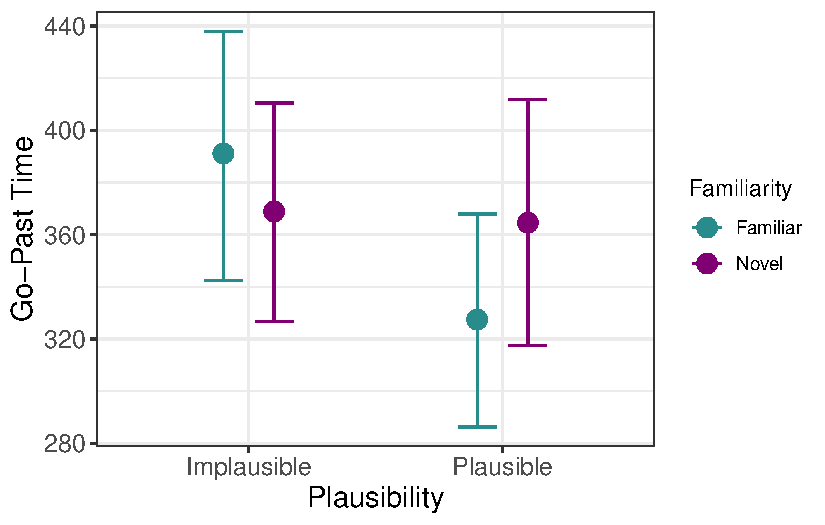
\includegraphics[width=0.8\linewidth,height=\textheight,keepaspectratio]{Chapters/Compound Nouns/staub_rep_ext_files/figure-pdf/fig-gopastn1staub-1.pdf}

}

\end{figure}%

\paragraph{N2}\label{n2-2}

Our results for the effects of plausibility and familiarity on go-past
times in the N2 region are described in Table~\ref{tbl-gopastn2staub}
and visualized in Figure~\ref{fig-gopastn2staub}.

Our results suggest an effect of familiarity such that familiar items
had shorter go-past times than novel items.

\begin{longtable}[]{@{}
  >{\raggedright\arraybackslash}p{(\linewidth - 10\tabcolsep) * \real{0.3378}}
  >{\raggedright\arraybackslash}p{(\linewidth - 10\tabcolsep) * \real{0.1216}}
  >{\raggedright\arraybackslash}p{(\linewidth - 10\tabcolsep) * \real{0.1351}}
  >{\raggedright\arraybackslash}p{(\linewidth - 10\tabcolsep) * \real{0.1081}}
  >{\raggedright\arraybackslash}p{(\linewidth - 10\tabcolsep) * \real{0.1081}}
  >{\raggedleft\arraybackslash}p{(\linewidth - 10\tabcolsep) * \real{0.1892}}@{}}

\caption{\label{tbl-gopastn2staub}Model results examining the effect of
plausibility and familiarity on go-past times for the N2 region.}

\tabularnewline

\toprule\noalign{}
\begin{minipage}[b]{\linewidth}\raggedright
\end{minipage} & \begin{minipage}[b]{\linewidth}\raggedright
Estimate
\end{minipage} & \begin{minipage}[b]{\linewidth}\raggedright
Est.Error
\end{minipage} & \begin{minipage}[b]{\linewidth}\raggedright
Q2.5
\end{minipage} & \begin{minipage}[b]{\linewidth}\raggedright
Q97.5
\end{minipage} & \begin{minipage}[b]{\linewidth}\raggedleft
\% Samples \textgreater{} 0
\end{minipage} \\
\midrule\noalign{}
\endhead
\bottomrule\noalign{}
\endlastfoot
Intercept & 351.825 & 21.876 & 308.493 & 394.204 & 100.000000 \\
Plausibility & 6.952 & 8.405 & -9.270 & 23.774 & 79.873333 \\
Familiarity & -17.433 & 13.362 & -44.885 & 7.492 & 8.966667 \\
Plausibility:Familiarity & -7.957 & 9.345 & -26.618 & 10.247 &
19.426667 \\

\end{longtable}

\begin{figure}[htbp]

\caption{\label{fig-gopastn2staub}Visualization of the effect of
plausibility and familiarity on go-past times for the N2 region.}

\centering{

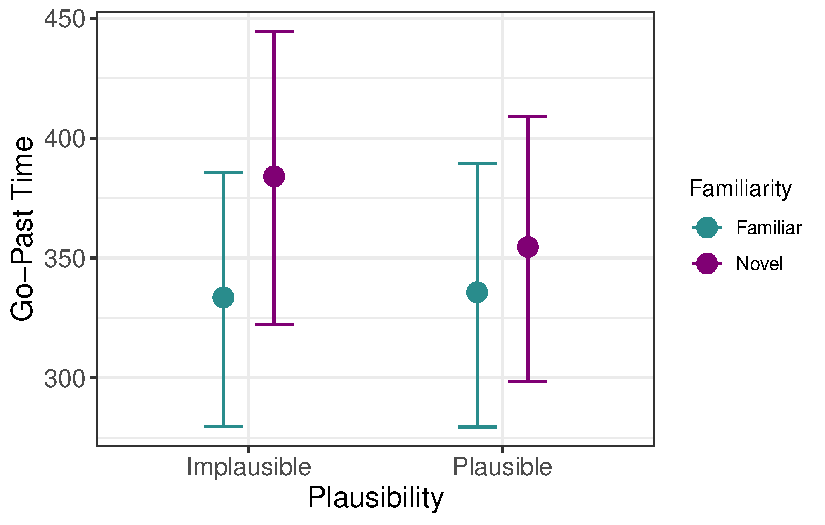
\includegraphics[width=0.8\linewidth,height=\textheight,keepaspectratio]{Chapters/Compound Nouns/staub_rep_ext_files/figure-pdf/fig-gopastn2staub-1.pdf}

}

\end{figure}%

\subsubsection{First-Pass Regression}\label{first-pass-regression}

\paragraph{N1}\label{n1-3}

Our results for the effects of plausibility and familiarity on
first-pass regressions in the N1 region are described in
Table~\ref{tbl-firstpassn1} and visualized in
Figure~\ref{fig-firstpassn1}.

Our results suggest an effect of plausibility on first pass regressions
for the N1 region such that implausible items had more first-pass
regressions than plausible items.

\begin{longtable}[]{@{}
  >{\raggedright\arraybackslash}p{(\linewidth - 10\tabcolsep) * \real{0.3472}}
  >{\raggedright\arraybackslash}p{(\linewidth - 10\tabcolsep) * \real{0.1250}}
  >{\raggedright\arraybackslash}p{(\linewidth - 10\tabcolsep) * \real{0.1389}}
  >{\raggedright\arraybackslash}p{(\linewidth - 10\tabcolsep) * \real{0.0972}}
  >{\raggedright\arraybackslash}p{(\linewidth - 10\tabcolsep) * \real{0.0972}}
  >{\raggedleft\arraybackslash}p{(\linewidth - 10\tabcolsep) * \real{0.1944}}@{}}

\caption{\label{tbl-firstpassn1staub}Model results examining the effect
of plausibility and familiarity on first-pass regression for the N1
region.}

\tabularnewline

\toprule\noalign{}
\begin{minipage}[b]{\linewidth}\raggedright
\end{minipage} & \begin{minipage}[b]{\linewidth}\raggedright
Estimate
\end{minipage} & \begin{minipage}[b]{\linewidth}\raggedright
Est.Error
\end{minipage} & \begin{minipage}[b]{\linewidth}\raggedright
Q2.5
\end{minipage} & \begin{minipage}[b]{\linewidth}\raggedright
Q97.5
\end{minipage} & \begin{minipage}[b]{\linewidth}\raggedleft
\% Samples \textgreater{} 0
\end{minipage} \\
\midrule\noalign{}
\endhead
\bottomrule\noalign{}
\endlastfoot
Intercept & -1.986 & 0.180 & -2.347 & -1.642 & 0.000 \\
Plausibility & 0.157 & 0.089 & -0.014 & 0.332 & 96.375 \\
Familiarity & 0.017 & 0.088 & -0.152 & 0.188 & 57.800 \\
Plausibility:Familiarity & 0.056 & 0.089 & -0.121 & 0.232 & 74.500 \\

\end{longtable}

\begin{figure}[htbp]

\caption{\label{fig-firstpassn1staub}Visualization of the effect of
plausibility and familiarity on first-pass regression for the N1
region.}

\centering{

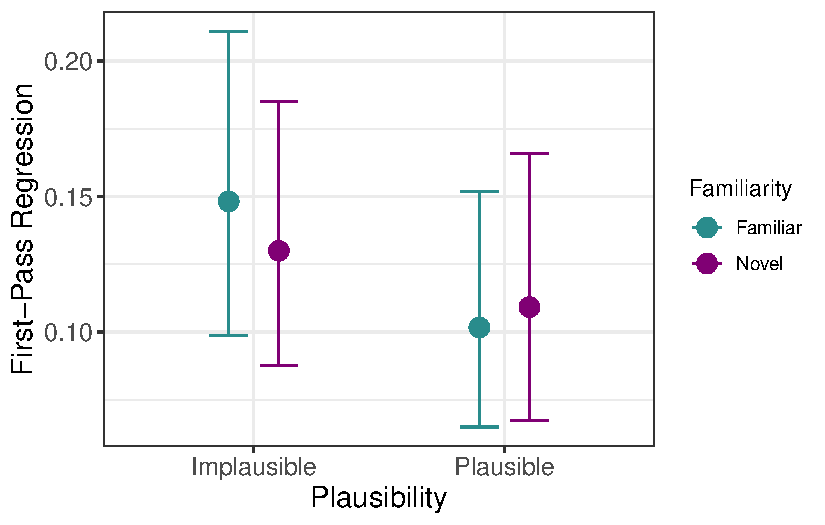
\includegraphics[width=0.8\linewidth,height=\textheight,keepaspectratio]{Chapters/Compound Nouns/staub_rep_ext_files/figure-pdf/fig-firstpassn1staub-1.pdf}

}

\end{figure}%

\paragraph{N2}\label{n2-3}

Our results for the effects of plausibility and familiarity on
first-pass regressions in the N2 region are described in
Table~\ref{tbl-firstpassn2} and visualized in
Figure~\ref{fig-firstpassn2}.

Our results suggest an effect of familiarity on first pass-regressions
for the N2 region suggesting that familiar items had fewer first-pass
regressions than novel items.

\begin{longtable}[]{@{}
  >{\raggedright\arraybackslash}p{(\linewidth - 10\tabcolsep) * \real{0.3472}}
  >{\raggedright\arraybackslash}p{(\linewidth - 10\tabcolsep) * \real{0.1250}}
  >{\raggedright\arraybackslash}p{(\linewidth - 10\tabcolsep) * \real{0.1389}}
  >{\raggedright\arraybackslash}p{(\linewidth - 10\tabcolsep) * \real{0.0972}}
  >{\raggedright\arraybackslash}p{(\linewidth - 10\tabcolsep) * \real{0.0972}}
  >{\raggedleft\arraybackslash}p{(\linewidth - 10\tabcolsep) * \real{0.1944}}@{}}

\caption{\label{tbl-firstpassn2staub}Model results examining the effect
of plausibility and familiarity on first-pass regression for the N2
region.}

\tabularnewline

\toprule\noalign{}
\begin{minipage}[b]{\linewidth}\raggedright
\end{minipage} & \begin{minipage}[b]{\linewidth}\raggedright
Estimate
\end{minipage} & \begin{minipage}[b]{\linewidth}\raggedright
Est.Error
\end{minipage} & \begin{minipage}[b]{\linewidth}\raggedright
Q2.5
\end{minipage} & \begin{minipage}[b]{\linewidth}\raggedright
Q97.5
\end{minipage} & \begin{minipage}[b]{\linewidth}\raggedleft
\% Samples \textgreater{} 0
\end{minipage} \\
\midrule\noalign{}
\endhead
\bottomrule\noalign{}
\endlastfoot
Intercept & -2.307 & 0.212 & -2.748 & -1.910 & 0.000 \\
Plausibility & 0.074 & 0.092 & -0.103 & 0.256 & 78.450 \\
Familiarity & -0.140 & 0.118 & -0.371 & 0.096 & 11.575 \\
Plausibility:Familiarity & -0.004 & 0.088 & -0.179 & 0.168 & 48.575 \\

\end{longtable}

\begin{figure}[htbp]

\caption{\label{fig-firstpassn2staub}Visualization of the effect of
plausibility and familiarity on first-pass regression for the N2
region.}

\centering{

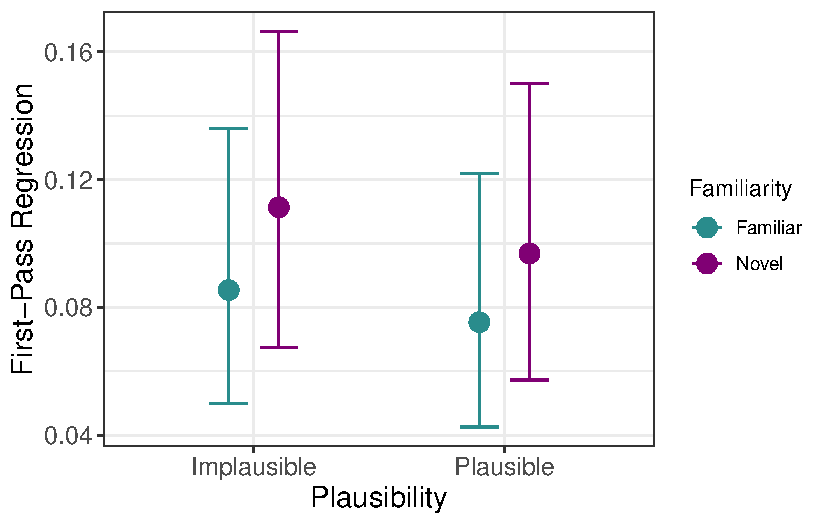
\includegraphics[width=0.8\linewidth,height=\textheight,keepaspectratio]{Chapters/Compound Nouns/staub_rep_ext_files/figure-pdf/fig-firstpassn2staub-1.pdf}

}

\end{figure}%

\subsection{Discussion}\label{discussion-2}

Experiment 3 demonstrates that readers have longer first-fixation times,
longer go-past times, and more first-pass regressions in implausible
contexts than in plausible contexts. Further, we find an interaction
effect in the opposite direction from predicted for go-past times: the
effect of plausibility is greater for familiar items than in novel
items. We will expand on this result in the Conclusion section.

\section{Experiment 4}\label{experiment-4}

In Experiment 4, we replicate the results we found in Experiment 2 using
eye-tracking.

\subsection{Methods}\label{methods-3}

\subsubsection{Participants}\label{participants-3}

56 native English speakers were recruited from the University of
California, Davis subjects pool. They were given course credit in
exchange for their participation. All participants had normal or
corrected vision.

\subsubsection{Materials}\label{materials-1}

The materials here were identical to those in Experiment 2.

\subsubsection{Procedure}\label{procedure-2}

We recorded participants' eye movements using the Eyelink 1000 Plus. We
recorded pupil movements from the right eye. Participants were seated
850mm away from the screen. Our screen resolution was 1920x1080, 531.3mm
in width, and 298.8mm in height.

Comprehension was checked for non-experimental trials and participants
below 80\% accuracy were excluded. Out of our 56 participants, 0 were
excluded for falling below the accuracy threshold.

\subsubsection{Analyses}\label{analyses-1}

Prior to our analyses, sentences with blinks were excluded and fixations
less than 80ms in duration and within one character of the nearest
fixation were merged into that fixation (following
\citeproc{ref-staubTimeCoursePlausibility2007}{Staub et al., 2007}). For
our regions of interest (the first noun and the second noun in the
compound noun), we computed first fixation duration, first pass time,
go-past time, and first-pass regression.

For each analysis, our independent variables were plausibility (high or
low) and (log) predictability (high or low) and their interaction. We
also included random slopes for condition and predictability by subject
and plausibility by compound noun as well as intercepts for subject and
compound noun. For each of our models, we used sum-coding, where the
intercept represents the grand mean and the fixed-effect coefficient
estimates represent the distance from the grand mean.

\subsection{Results}\label{results-3}

\subsubsection{First Fixation Times}\label{first-fixation-times-1}

\paragraph{N1}\label{n1-4}

First, we examined the effects of plausibility and predictability on
first fixation times for the first noun. Note that in our case, since
plausibility was coded as -1 for plausible and 1 for implausible, a
positive coefficient estimate of plausibility corresponds to longer
fixation times for implausible items. Additionally, following Houghton
et al.
(\citeproc{ref-houghtonTaskdependentConsequencesDisfluency2024}{2024})
we also report the percentage of posterior samples greater than zero.
Our model results can be found below in Table~\ref{tbl-firstfixn1} and a
visualization can be found in Figure~\ref{fig-firstfixn1}.

Our results for first-fixation times, while non-significant, do show an
interesting trend, with the effect of plausibility in the expected
direction (although with only \textasciitilde78\% samples greater than
zero). Further, we found a small but meaningful interaction effect such
that the readers' first-fixation times of low-predictability items was
affected more by the local implausibility than the high-predictability
items were.

\begin{longtable}[]{@{}
  >{\raggedright\arraybackslash}p{(\linewidth - 10\tabcolsep) * \real{0.3636}}
  >{\raggedright\arraybackslash}p{(\linewidth - 10\tabcolsep) * \real{0.1169}}
  >{\raggedright\arraybackslash}p{(\linewidth - 10\tabcolsep) * \real{0.1299}}
  >{\raggedright\arraybackslash}p{(\linewidth - 10\tabcolsep) * \real{0.1039}}
  >{\raggedright\arraybackslash}p{(\linewidth - 10\tabcolsep) * \real{0.1039}}
  >{\raggedleft\arraybackslash}p{(\linewidth - 10\tabcolsep) * \real{0.1818}}@{}}

\caption{\label{tbl-firstfixn1}Model results examining the effect of
plausibility and predictability on first fixation times for the N1
region.}

\tabularnewline

\toprule\noalign{}
\begin{minipage}[b]{\linewidth}\raggedright
\end{minipage} & \begin{minipage}[b]{\linewidth}\raggedright
Estimate
\end{minipage} & \begin{minipage}[b]{\linewidth}\raggedright
Est.Error
\end{minipage} & \begin{minipage}[b]{\linewidth}\raggedright
Q2.5
\end{minipage} & \begin{minipage}[b]{\linewidth}\raggedright
Q97.5
\end{minipage} & \begin{minipage}[b]{\linewidth}\raggedleft
\% Samples \textgreater{} 0
\end{minipage} \\
\midrule\noalign{}
\endhead
\bottomrule\noalign{}
\endlastfoot
Intercept & 231.016 & 4.433 & 222.356 & 239.502 & 100.00 \\
Plausibility & 1.661 & 2.020 & -2.289 & 5.695 & 78.95 \\
Predictability & 2.782 & 2.870 & -2.804 & 8.532 & 83.75 \\
Plausibility:Predictability & -3.473 & 2.012 & -7.418 & 0.522 & 4.15 \\

\end{longtable}

\begin{figure}[htbp]

\caption{\label{fig-firstfixn1}Visualization of the effects of
plausibility and predictability on first fixation times for the N1
region.}

\centering{

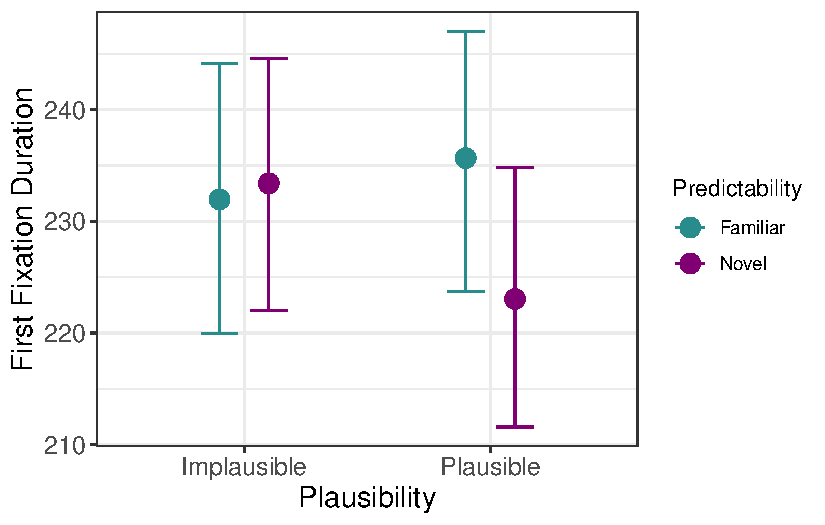
\includegraphics[width=0.8\linewidth,height=\textheight,keepaspectratio]{Chapters/Compound Nouns/staub_rep_ext_files/figure-pdf/fig-firstfixn1-1.pdf}

}

\end{figure}%

\paragraph{N2}\label{n2-4}

Our results for the effects of plausibility and predictability on first
fixation times in the N2 region are described in
Table~\ref{tbl-firstfixn2} and visualized in Figure~\ref{fig-firstfixn2}

Our results demonstrate an effect of predictability on the first
fixation times of the second noun in the compound noun. This is rather
unsurprising because in the present study predictability is a measure of
how expected the second noun is given the first. There also is not much
of a plausibility effect on the N2, which is also not particularly
surprising because the second noun eliminates the local implausibility
making both sentences plausible at the N2 region.

\begin{longtable}[]{@{}
  >{\raggedright\arraybackslash}p{(\linewidth - 10\tabcolsep) * \real{0.3636}}
  >{\raggedright\arraybackslash}p{(\linewidth - 10\tabcolsep) * \real{0.1169}}
  >{\raggedright\arraybackslash}p{(\linewidth - 10\tabcolsep) * \real{0.1299}}
  >{\raggedright\arraybackslash}p{(\linewidth - 10\tabcolsep) * \real{0.1039}}
  >{\raggedright\arraybackslash}p{(\linewidth - 10\tabcolsep) * \real{0.1039}}
  >{\raggedleft\arraybackslash}p{(\linewidth - 10\tabcolsep) * \real{0.1818}}@{}}

\caption{\label{tbl-firstfixn2}Model results examining the effect of
plausibility and predictability on first fixation times for the N2
region.}

\tabularnewline

\toprule\noalign{}
\begin{minipage}[b]{\linewidth}\raggedright
\end{minipage} & \begin{minipage}[b]{\linewidth}\raggedright
Estimate
\end{minipage} & \begin{minipage}[b]{\linewidth}\raggedright
Est.Error
\end{minipage} & \begin{minipage}[b]{\linewidth}\raggedright
Q2.5
\end{minipage} & \begin{minipage}[b]{\linewidth}\raggedright
Q97.5
\end{minipage} & \begin{minipage}[b]{\linewidth}\raggedleft
\% Samples \textgreater{} 0
\end{minipage} \\
\midrule\noalign{}
\endhead
\bottomrule\noalign{}
\endlastfoot
Intercept & 234.448 & 4.864 & 224.479 & 243.767 & 100.000 \\
Plausibility & -2.151 & 2.973 & -8.132 & 3.685 & 23.225 \\
Predictability & -4.136 & 2.988 & -9.887 & 1.887 & 8.575 \\
Plausibility:Predictability & -2.928 & 3.012 & -8.920 & 2.967 &
16.075 \\

\end{longtable}

\begin{figure}[htbp]

\caption{\label{fig-firstfixn2}Visualization of the effects of
plausibility and predictability on first fixation times for the N2
region.}

\centering{

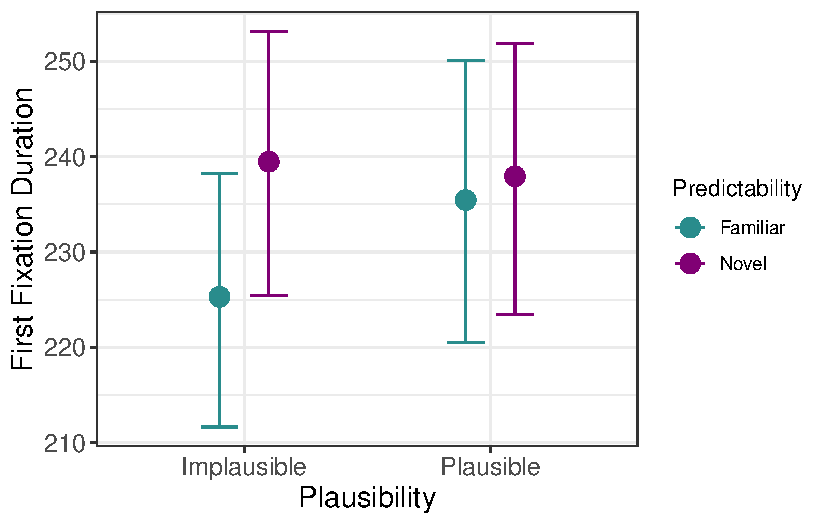
\includegraphics[width=0.8\linewidth,height=\textheight,keepaspectratio]{Chapters/Compound Nouns/staub_rep_ext_files/figure-pdf/fig-firstfixn2-1.pdf}

}

\end{figure}%

\subsubsection{Gaze/First-Pass Time}\label{gazefirst-pass-time-1}

\paragraph{N1}\label{n1-5}

Our results for the effects of plausibility and predictability on
gaze/first-pass times for the N1 region are presented in
Table~\ref{tbl-gazen1} and visualized in Figure~\ref{fig-gazen1}.

Our results demonstrate no effect of either plausibility or
predictability on the gaze times at the N1 region. We further examined
our filler items to rule out an error with the eye-tracker. Our filler
items contain a frequency manipulation and an analysis of the filler
items demonstrated that the frequency manipulation did effect gaze times
in our filler items, suggesting that the results here are not due to any
malfunction of the eye-tracker or cleaning procedure. We report the
effects found in the filler items at the end of this section.

\begin{longtable}[]{@{}
  >{\raggedright\arraybackslash}p{(\linewidth - 10\tabcolsep) * \real{0.3636}}
  >{\raggedright\arraybackslash}p{(\linewidth - 10\tabcolsep) * \real{0.1169}}
  >{\raggedright\arraybackslash}p{(\linewidth - 10\tabcolsep) * \real{0.1299}}
  >{\raggedright\arraybackslash}p{(\linewidth - 10\tabcolsep) * \real{0.1039}}
  >{\raggedright\arraybackslash}p{(\linewidth - 10\tabcolsep) * \real{0.1039}}
  >{\raggedleft\arraybackslash}p{(\linewidth - 10\tabcolsep) * \real{0.1818}}@{}}

\caption{\label{tbl-gazen1}Model results examining the effect of
plausibility and predictability on Gaze/first-pass times for the N1
region.}

\tabularnewline

\toprule\noalign{}
\begin{minipage}[b]{\linewidth}\raggedright
\end{minipage} & \begin{minipage}[b]{\linewidth}\raggedright
Estimate
\end{minipage} & \begin{minipage}[b]{\linewidth}\raggedright
Est.Error
\end{minipage} & \begin{minipage}[b]{\linewidth}\raggedright
Q2.5
\end{minipage} & \begin{minipage}[b]{\linewidth}\raggedright
Q97.5
\end{minipage} & \begin{minipage}[b]{\linewidth}\raggedleft
\% Samples \textgreater{} 0
\end{minipage} \\
\midrule\noalign{}
\endhead
\bottomrule\noalign{}
\endlastfoot
Intercept & 264.141 & 8.422 & 246.898 & 280.601 & 100.000 \\
Plausibility & -0.001 & 0.203 & -0.385 & 0.413 & 49.075 \\
Predictability & 0.005 & 0.198 & -0.394 & 0.387 & 51.475 \\
Plausibility:Predictability & -0.010 & 0.202 & -0.411 & 0.382 &
48.100 \\

\end{longtable}

\newpage

\begin{figure}[htbp]

\caption{\label{fig-gazen1}Visualization of the effects of plausibility
and predictability on Gaze/first-pass times for the N1 region.}

\centering{

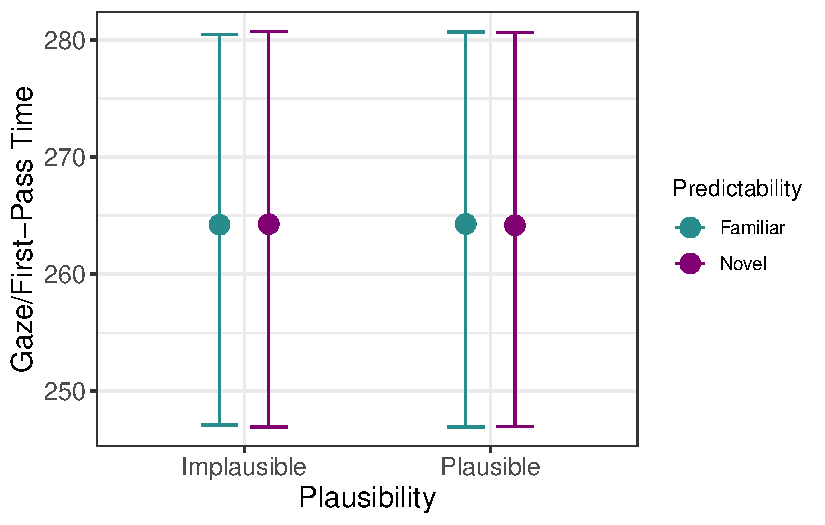
\includegraphics[width=0.8\linewidth,height=\textheight,keepaspectratio]{Chapters/Compound Nouns/staub_rep_ext_files/figure-pdf/fig-gazen1-1.pdf}

}

\end{figure}%

\paragraph{N2}\label{n2-5}

Our results for the effects of plausibility and predictability on
gaze/first-pass times for the N2 region are presented in
Table~\ref{tbl-gazen1} and visualized in Figure~\ref{fig-gazen1}.

Our results demonstrate no effect of either plausibility or
predictability on the gaze times at the N2 region. This is surprising
because the effect of predictability should facilitate reading at the
N2.

\begin{longtable}[]{@{}
  >{\raggedright\arraybackslash}p{(\linewidth - 10\tabcolsep) * \real{0.3636}}
  >{\raggedright\arraybackslash}p{(\linewidth - 10\tabcolsep) * \real{0.1169}}
  >{\raggedright\arraybackslash}p{(\linewidth - 10\tabcolsep) * \real{0.1299}}
  >{\raggedright\arraybackslash}p{(\linewidth - 10\tabcolsep) * \real{0.1039}}
  >{\raggedright\arraybackslash}p{(\linewidth - 10\tabcolsep) * \real{0.1039}}
  >{\raggedleft\arraybackslash}p{(\linewidth - 10\tabcolsep) * \real{0.1818}}@{}}

\caption{\label{tbl-gazen2}Model results examining the effect of
plausibility and predictability on Gaze/first-pass times for the N2
region.}

\tabularnewline

\toprule\noalign{}
\begin{minipage}[b]{\linewidth}\raggedright
\end{minipage} & \begin{minipage}[b]{\linewidth}\raggedright
Estimate
\end{minipage} & \begin{minipage}[b]{\linewidth}\raggedright
Est.Error
\end{minipage} & \begin{minipage}[b]{\linewidth}\raggedright
Q2.5
\end{minipage} & \begin{minipage}[b]{\linewidth}\raggedright
Q97.5
\end{minipage} & \begin{minipage}[b]{\linewidth}\raggedleft
\% Samples \textgreater{} 0
\end{minipage} \\
\midrule\noalign{}
\endhead
\bottomrule\noalign{}
\endlastfoot
Intercept & 253.757 & 6.071 & 241.726 & 265.767 & 100.000 \\
Plausibility & -0.003 & 0.100 & -0.196 & 0.192 & 48.825 \\
Predictability & -0.003 & 0.101 & -0.207 & 0.190 & 48.625 \\
Plausibility:Predictability & 0.003 & 0.100 & -0.199 & 0.202 & 51.625 \\

\end{longtable}

\begin{figure}[htbp]

\caption{\label{fig-gazen2}Visualization of the effects of plausibility
and predictability on Gaze/first-pass times for the N2 region.}

\centering{

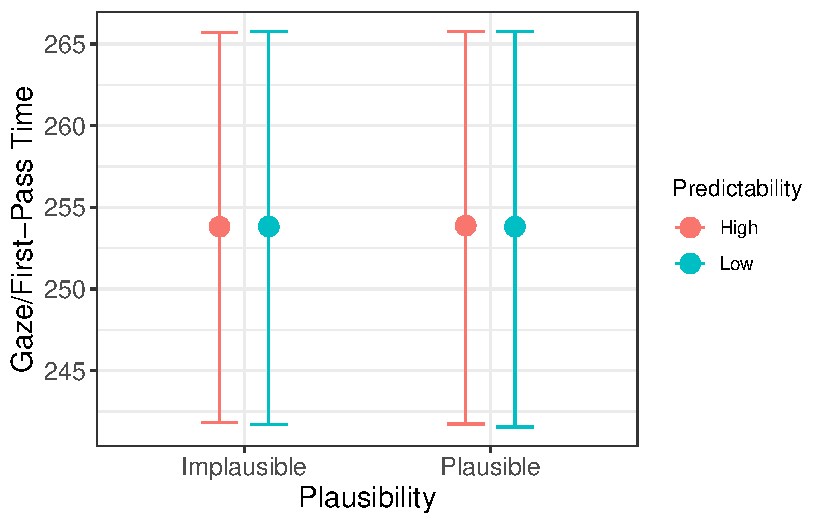
\includegraphics[width=0.8\linewidth,height=\textheight,keepaspectratio]{Chapters/Compound Nouns/staub_rep_ext_files/figure-pdf/fig-gazen2-1.pdf}

}

\end{figure}%

\subsubsection{Go-Past Time}\label{go-past-time-1}

\paragraph{N1}\label{n1-6}

Our results for the effects of plausibility and predictability on
go-past times for the N1 region are presented in
Table~\ref{tbl-gopastn1} and visualized in Figure~\ref{fig-gopastn1}.

The results for go-past times show no effect of predictability and
plausibility on the N1 region.

\begin{longtable}[]{@{}
  >{\raggedright\arraybackslash}p{(\linewidth - 10\tabcolsep) * \real{0.3636}}
  >{\raggedright\arraybackslash}p{(\linewidth - 10\tabcolsep) * \real{0.1169}}
  >{\raggedright\arraybackslash}p{(\linewidth - 10\tabcolsep) * \real{0.1299}}
  >{\raggedright\arraybackslash}p{(\linewidth - 10\tabcolsep) * \real{0.1039}}
  >{\raggedright\arraybackslash}p{(\linewidth - 10\tabcolsep) * \real{0.1039}}
  >{\raggedleft\arraybackslash}p{(\linewidth - 10\tabcolsep) * \real{0.1818}}@{}}

\caption{\label{tbl-gopastn1}Model results examining the effect of
plausibility and predictability on go-past times for the N1 region.}

\tabularnewline

\toprule\noalign{}
\begin{minipage}[b]{\linewidth}\raggedright
\end{minipage} & \begin{minipage}[b]{\linewidth}\raggedright
Estimate
\end{minipage} & \begin{minipage}[b]{\linewidth}\raggedright
Est.Error
\end{minipage} & \begin{minipage}[b]{\linewidth}\raggedright
Q2.5
\end{minipage} & \begin{minipage}[b]{\linewidth}\raggedright
Q97.5
\end{minipage} & \begin{minipage}[b]{\linewidth}\raggedleft
\% Samples \textgreater{} 0
\end{minipage} \\
\midrule\noalign{}
\endhead
\bottomrule\noalign{}
\endlastfoot
Intercept & 357.207 & 16.452 & 325.205 & 388.957 & 100.00000 \\
Plausibility & 0.018 & 0.197 & -0.367 & 0.400 & 54.05000 \\
Predictability & 0.005 & 0.200 & -0.390 & 0.394 & 50.10000 \\
Plausibility:Predictability & -0.000 & 0.200 & -0.392 & 0.393 &
49.76667 \\

\end{longtable}

\begin{figure}[htbp]

\caption{\label{fig-gopastn1}Visualization of the effect of plausibility
and predictability on go-past times for the N1 region.}

\centering{

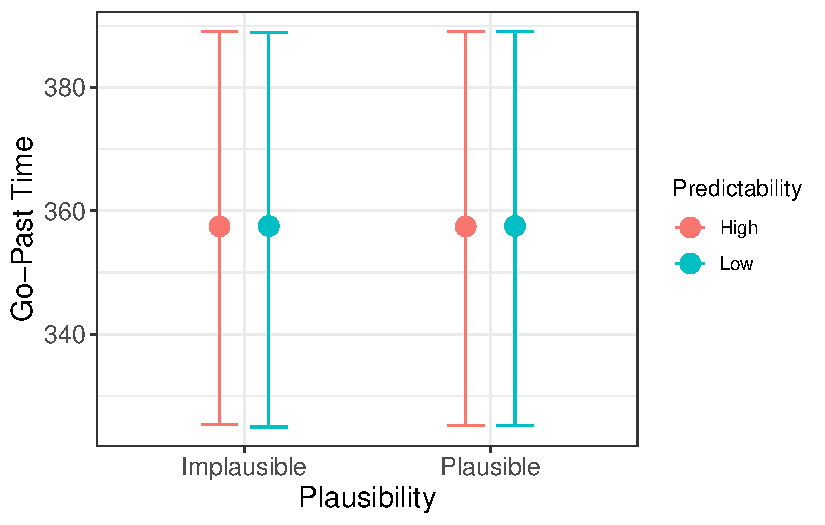
\includegraphics[width=0.8\linewidth,height=\textheight,keepaspectratio]{Chapters/Compound Nouns/staub_rep_ext_files/figure-pdf/fig-gopastn1-1.pdf}

}

\end{figure}%

\paragraph{N2}\label{n2-6}

Our results for the effects of plausibility and predictability on
go-past times for the N2 region are presented in
Table~\ref{tbl-gopastn2} and visualized in Figure~\ref{fig-gopastn2}.

Our results for the N2 region similarly show no effect of predictability
and plausibility on go-past times.

\begin{longtable}[]{@{}
  >{\raggedright\arraybackslash}p{(\linewidth - 10\tabcolsep) * \real{0.3636}}
  >{\raggedright\arraybackslash}p{(\linewidth - 10\tabcolsep) * \real{0.1169}}
  >{\raggedright\arraybackslash}p{(\linewidth - 10\tabcolsep) * \real{0.1299}}
  >{\raggedright\arraybackslash}p{(\linewidth - 10\tabcolsep) * \real{0.1039}}
  >{\raggedright\arraybackslash}p{(\linewidth - 10\tabcolsep) * \real{0.1039}}
  >{\raggedleft\arraybackslash}p{(\linewidth - 10\tabcolsep) * \real{0.1818}}@{}}

\caption{\label{tbl-gopastn2}Model results examining the effect of
plausibility and predictability on go-past times for the N2 region.}

\tabularnewline

\toprule\noalign{}
\begin{minipage}[b]{\linewidth}\raggedright
\end{minipage} & \begin{minipage}[b]{\linewidth}\raggedright
Estimate
\end{minipage} & \begin{minipage}[b]{\linewidth}\raggedright
Est.Error
\end{minipage} & \begin{minipage}[b]{\linewidth}\raggedright
Q2.5
\end{minipage} & \begin{minipage}[b]{\linewidth}\raggedright
Q97.5
\end{minipage} & \begin{minipage}[b]{\linewidth}\raggedleft
\% Samples \textgreater{} 0
\end{minipage} \\
\midrule\noalign{}
\endhead
\bottomrule\noalign{}
\endlastfoot
Intercept & 342.737 & 12.866 & 317.685 & 367.649 & 100.000 \\
Plausibility & -0.005 & 0.099 & -0.202 & 0.195 & 47.600 \\
Predictability & -0.001 & 0.100 & -0.198 & 0.195 & 50.000 \\
Plausibility:Predictability & -0.002 & 0.100 & -0.192 & 0.198 &
49.025 \\

\end{longtable}

\begin{figure}[htbp]

\caption{\label{fig-gopastn2}Visualization of the effect of plausibility
and predictability on go-past times for the N2 region.}

\centering{

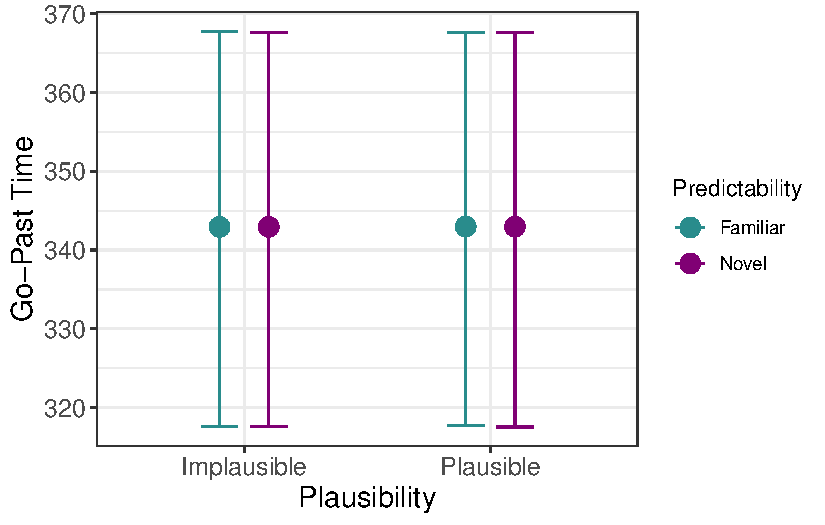
\includegraphics[width=0.8\linewidth,height=\textheight,keepaspectratio]{Chapters/Compound Nouns/staub_rep_ext_files/figure-pdf/fig-gopastn2-1.pdf}

}

\end{figure}%

\subsubsection{First-Pass Regression}\label{first-pass-regression-1}

\paragraph{N1}\label{n1-7}

Our results for the effects of predictability and plausibility on the
first-pass regressions on the N1 region are presented in
Table~\ref{tbl-firstpassn1} and visualized in
Figure~\ref{fig-firstpassn1}.

Our results suggest that readers are more likely to regress after the
first fixation in the implausible condition compared to the plausible
condition. Further, this plausibility effect is larger for
high-predictability items than low predictability items. This is
surprising because predictability is a measure of the N2, not the N1 and
if readers are anticipating the N2 then it should alleviate the local
implausibility at the N1 (which would result in a negative interaction
effect, i.e.~the opposite trend from what we see here).

\begin{longtable}[]{@{}
  >{\raggedright\arraybackslash}p{(\linewidth - 10\tabcolsep) * \real{0.3733}}
  >{\raggedright\arraybackslash}p{(\linewidth - 10\tabcolsep) * \real{0.1200}}
  >{\raggedright\arraybackslash}p{(\linewidth - 10\tabcolsep) * \real{0.1333}}
  >{\raggedright\arraybackslash}p{(\linewidth - 10\tabcolsep) * \real{0.0933}}
  >{\raggedright\arraybackslash}p{(\linewidth - 10\tabcolsep) * \real{0.0933}}
  >{\raggedleft\arraybackslash}p{(\linewidth - 10\tabcolsep) * \real{0.1867}}@{}}

\caption{\label{tbl-firstpassn1}Model results examining the effect of
plausibility and predictability on first-pass regression for the N1
region.}

\tabularnewline

\toprule\noalign{}
\begin{minipage}[b]{\linewidth}\raggedright
\end{minipage} & \begin{minipage}[b]{\linewidth}\raggedright
Estimate
\end{minipage} & \begin{minipage}[b]{\linewidth}\raggedright
Est.Error
\end{minipage} & \begin{minipage}[b]{\linewidth}\raggedright
Q2.5
\end{minipage} & \begin{minipage}[b]{\linewidth}\raggedright
Q97.5
\end{minipage} & \begin{minipage}[b]{\linewidth}\raggedleft
\% Samples \textgreater{} 0
\end{minipage} \\
\midrule\noalign{}
\endhead
\bottomrule\noalign{}
\endlastfoot
Intercept & -1.645 & 0.151 & -1.948 & -1.358 & 0.000 \\
Plausibility & 0.199 & 0.080 & 0.041 & 0.357 & 99.375 \\
Predictability & -0.049 & 0.086 & -0.214 & 0.123 & 27.750 \\
Plausibility:Predictability & 0.128 & 0.075 & -0.019 & 0.275 & 96.025 \\

\end{longtable}

\begin{figure}[htbp]

\caption{\label{fig-firstpassn1}Visualization of the effect of
plausibility and predictability on first-pass regression for the N1
region.}

\centering{

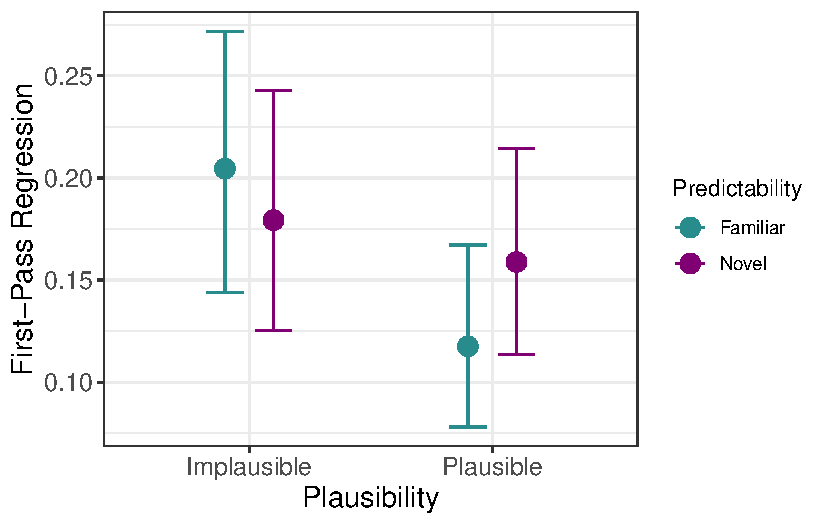
\includegraphics[width=0.8\linewidth,height=\textheight,keepaspectratio]{Chapters/Compound Nouns/staub_rep_ext_files/figure-pdf/fig-firstpassn1-1.pdf}

}

\end{figure}%

\paragraph{N2}\label{n2-7}

Our results for the effects of predictability and plausibility on
first-pass regressions in the N1 region are presented in
Table~\ref{tbl-firstpassn2} and visualized in
Figure~\ref{fig-firstpassn2}.

Our results no effect of predictability or plausibility. In other words,
unexpectedly high-predictability items had similar first-pass
regressions as low-predictability items in the N2 region.

\begin{longtable}[]{@{}
  >{\raggedright\arraybackslash}p{(\linewidth - 10\tabcolsep) * \real{0.3733}}
  >{\raggedright\arraybackslash}p{(\linewidth - 10\tabcolsep) * \real{0.1200}}
  >{\raggedright\arraybackslash}p{(\linewidth - 10\tabcolsep) * \real{0.1333}}
  >{\raggedright\arraybackslash}p{(\linewidth - 10\tabcolsep) * \real{0.0933}}
  >{\raggedright\arraybackslash}p{(\linewidth - 10\tabcolsep) * \real{0.0933}}
  >{\raggedleft\arraybackslash}p{(\linewidth - 10\tabcolsep) * \real{0.1867}}@{}}

\caption{\label{tbl-firstpassn2}Model results examining the effect of
plausibility and predictability on first-pass regression for the N2
region.}

\tabularnewline

\toprule\noalign{}
\begin{minipage}[b]{\linewidth}\raggedright
\end{minipage} & \begin{minipage}[b]{\linewidth}\raggedright
Estimate
\end{minipage} & \begin{minipage}[b]{\linewidth}\raggedright
Est.Error
\end{minipage} & \begin{minipage}[b]{\linewidth}\raggedright
Q2.5
\end{minipage} & \begin{minipage}[b]{\linewidth}\raggedright
Q97.5
\end{minipage} & \begin{minipage}[b]{\linewidth}\raggedleft
\% Samples \textgreater{} 0
\end{minipage} \\
\midrule\noalign{}
\endhead
\bottomrule\noalign{}
\endlastfoot
Intercept & -2.061 & 0.176 & -2.426 & -1.728 & 0.000 \\
Plausibility & -0.026 & 0.106 & -0.241 & 0.184 & 40.625 \\
Predictability & -0.022 & 0.102 & -0.223 & 0.177 & 41.100 \\
Plausibility:Predictability & 0.049 & 0.097 & -0.136 & 0.239 & 69.975 \\

\end{longtable}

\newpage

\begin{figure}[htbp]

\caption{\label{fig-firstpassn2}Visualization of the effect of
plausibility and predictability on first-pass regression for the N2
region.}

\centering{

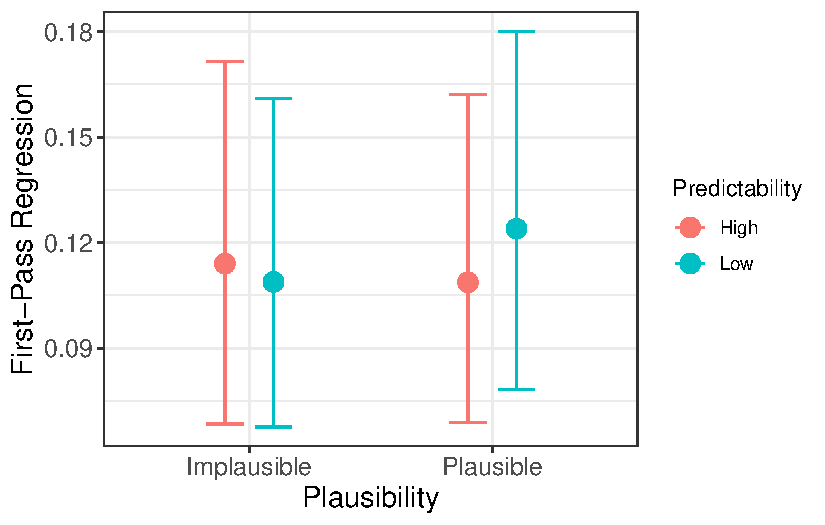
\includegraphics[width=0.8\linewidth,height=\textheight,keepaspectratio]{Chapters/Compound Nouns/staub_rep_ext_files/figure-pdf/fig-firstpassn2-1.pdf}

}

\end{figure}%

\subsubsection{Filler Items}\label{filler-items}

In order to confirm that our results weren't due to measurement error,
we used examined our filler items to sanity check our findings. Our
filler items contained a frequency manipulation where some items were
low-frequency and some were high-frequency. The Psycholinguistics
literature has demonstrated the robustness of the effects of frequency
on reading measures, thus we examined our filler items to confirm that
that the results for Gaze/First-Pass times and Go-Past time were not due
to measurement error.

\paragraph{First Fixation Times}\label{first-fixation-times-2}

Our results for the effects of frequency on first fixation times for our
filler items is presented in Table~\ref{tbl-firstfixationfiller} and
visualized in Figure~\ref{fig-firstfixationfiller}.

Our results, unsurprisingly, demonstrate longer first fixation times for
low frequency items compared to high frequency items.

\begin{longtable}[]{@{}lllllr@{}}

\caption{\label{tbl-firstfixationfiller}Model results examining the
effect of frequency on first fixation times in our filler materials.}

\tabularnewline

\toprule\noalign{}
& Estimate & Est.Error & Q2.5 & Q97.5 & \% Samples \textgreater{} 0 \\
\midrule\noalign{}
\endhead
\bottomrule\noalign{}
\endlastfoot
Intercept & 227.843 & 3.942 & 220.186 & 235.404 & 100.0 \\
Frequency & 4.011 & 1.848 & 0.414 & 7.642 & 98.5 \\

\end{longtable}

\begin{figure}[htbp]

\caption{\label{fig-firstfixationfiller}Visualization of the effect of
frequency on first fixation times in our filler materials.}

\centering{

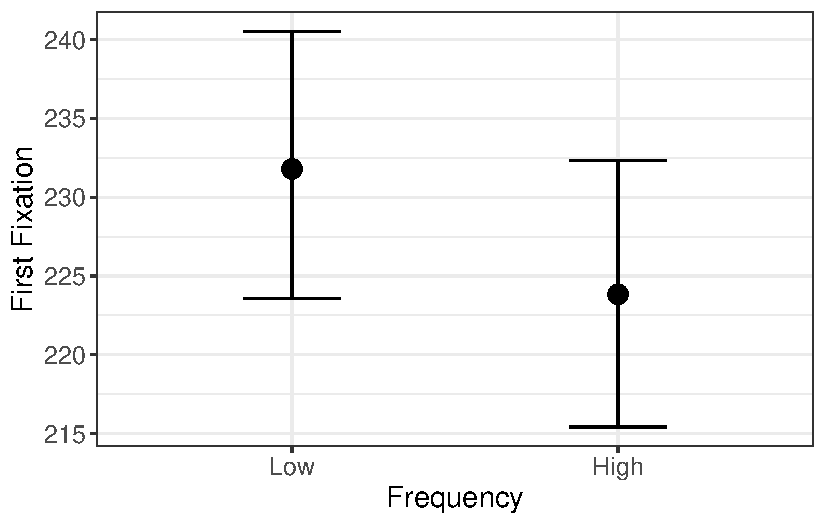
\includegraphics[width=0.6\linewidth,height=\textheight,keepaspectratio]{Chapters/Compound Nouns/staub_rep_ext_files/figure-pdf/fig-firstfixationfiller-1.pdf}

}

\end{figure}%

\paragraph{Gaze/First-Pass Time}\label{gazefirst-pass-time-2}

Our results for the effects of frequency on gaze/first-pass times for
our filler items is presented in Table~\ref{tbl-gazefiller} and
visualized in Figure~\ref{fig-gazefiller}.

Similarly, our results demonstrate longer gaze times for low-frequency
items compared to high-frequency ones. This suggests that the results we
found in Experiment 4 are not due to measurement error.

\begin{longtable}[]{@{}lllllr@{}}

\caption{\label{tbl-gazefiller}Model results examining the effect of
frequency on gaze/first-pass times in our filler materials.}

\tabularnewline

\toprule\noalign{}
& Estimate & Est.Error & Q2.5 & Q97.5 & \% Samples \textgreater{} 0 \\
\midrule\noalign{}
\endhead
\bottomrule\noalign{}
\endlastfoot
Intercept & 261.710 & 7.805 & 246.338 & 276.992 & 100.00000 \\
Frequency & 13.825 & 4.371 & 5.179 & 22.322 & 99.88333 \\

\end{longtable}

\begin{figure}[htbp]

\caption{\label{fig-gazefiller}Visualization of the effect of frequency
on gaze/first-pass times in our filler materials.}

\centering{

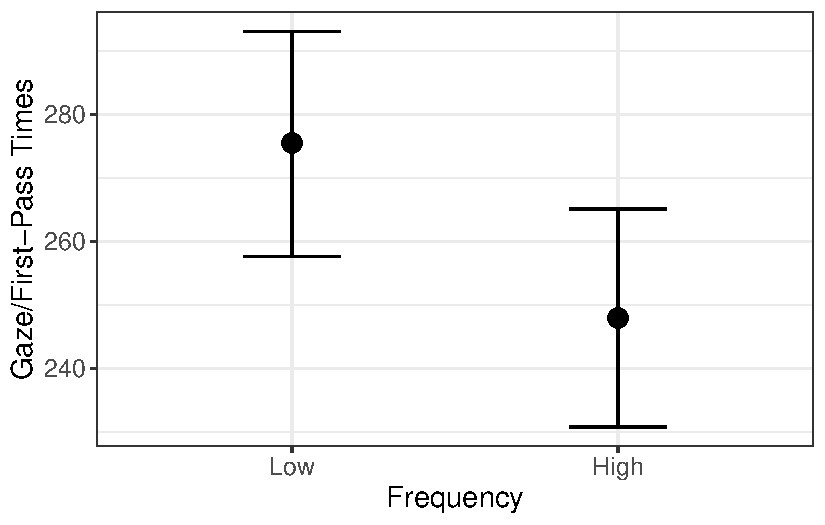
\includegraphics[width=0.6\linewidth,height=\textheight,keepaspectratio]{Chapters/Compound Nouns/staub_rep_ext_files/figure-pdf/fig-gazefiller-1.pdf}

}

\end{figure}%

\paragraph{Go-Past Time}\label{go-past-time-2}

Our results for the effects of frequency on go-past times for our filler
items is presented in Table~\ref{tbl-gopastfiller} and visualized in
Figure~\ref{fig-gopastfiller}.

For go-past times as well, we do find an effect such that low-frequency
items had longer go-past times. These results further confirm that the
results found in Experiment 4 were not due to measurement error.

\begin{longtable}[]{@{}lllllr@{}}

\caption{\label{tbl-gopastfiller}Model results examining the effect of
frequency on go-past times in our filler materials.}

\tabularnewline

\toprule\noalign{}
& Estimate & Est.Error & Q2.5 & Q97.5 & \% Samples \textgreater{} 0 \\
\midrule\noalign{}
\endhead
\bottomrule\noalign{}
\endlastfoot
Intercept & 368.199 & 17.340 & 334.329 & 402.836 & 100.0 \\
Frequency & 24.391 & 7.863 & 9.001 & 39.509 & 99.8 \\

\end{longtable}

\begin{figure}[htbp]

\caption{\label{fig-gopastfiller}Visualization of the effect of
frequency on go-past times in our filler materials.}

\centering{

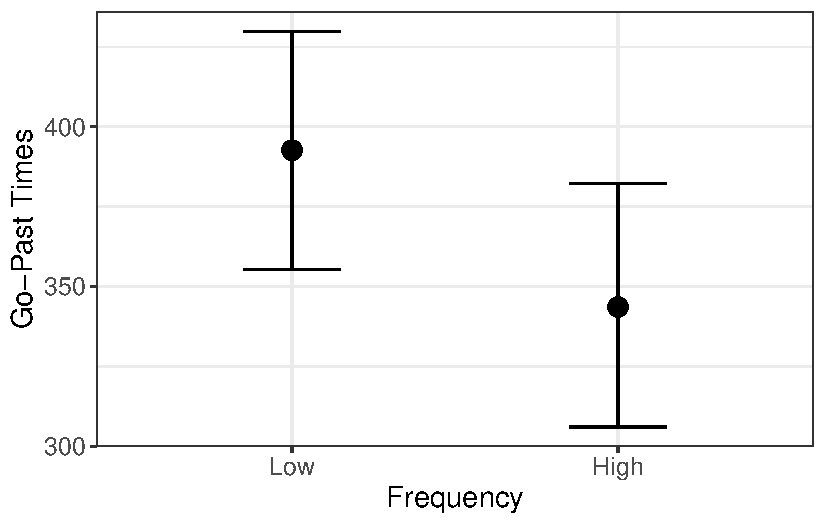
\includegraphics[width=0.6\linewidth,height=\textheight,keepaspectratio]{Chapters/Compound Nouns/staub_rep_ext_files/figure-pdf/fig-gopastfiller-1.pdf}

}

\end{figure}%

\paragraph{First-Pass Regression}\label{first-pass-regression-2}

Finally, our results for the first-pass regression rates of our filler
items is presented in Table~\ref{tbl-firstpassregressionfiller} and
visualized in Figure~\ref{fig-firstpassregressionfiller}.

The results of first-pass regressions demonstrate a greater rate of
first-pass regressions for low frequency items relative to high
frequency items. These results taken together suggest that the effects
of plausibility and predictability on each of the eye-tracking measures
was not a consequence of measurement error.

\begin{longtable}[]{@{}lllllr@{}}

\caption{\label{tbl-firstpassregressionfiller}Model results examining
the effect of frequency on first-pass regressions in our filler
materials.}

\tabularnewline

\toprule\noalign{}
& Estimate & Est.Error & Q2.5 & Q97.5 & \% Samples \textgreater{} 0 \\
\midrule\noalign{}
\endhead
\bottomrule\noalign{}
\endlastfoot
Intercept & -1.659 & 0.129 & -1.921 & -1.417 & 0.0 \\
Frequency & 0.156 & 0.058 & 0.044 & 0.271 & 99.6 \\

\end{longtable}

\begin{figure}[htbp]

\caption{\label{fig-firstpassregressionfiller}Visualization of the
effect of frequency on first-pass regressions in our filler materials.}

\centering{

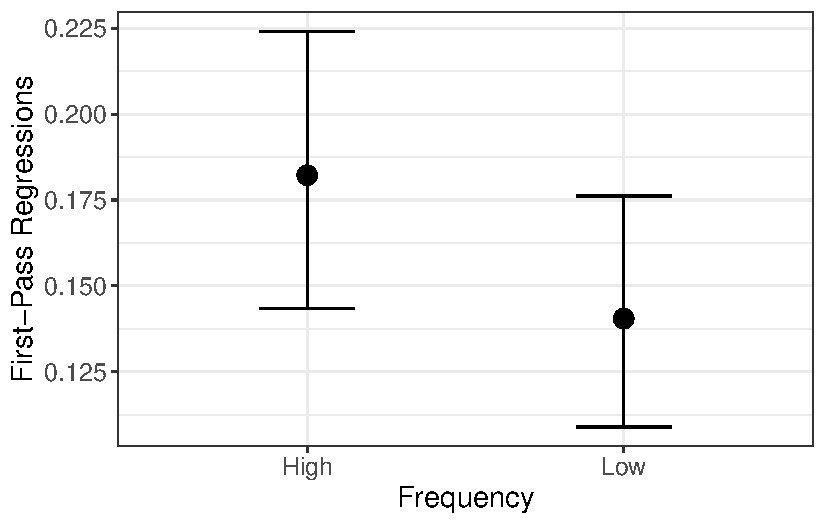
\includegraphics[width=0.6\linewidth,height=\textheight,keepaspectratio]{Chapters/Compound Nouns/staub_rep_ext_files/figure-pdf/fig-firstpassregressionfiller-1.pdf}

}

\end{figure}%

\subsection{Discussion}\label{discussion-3}

The results in Experiment 4 confirmed an effect of plausibility in
first-fixation times for low-predictability items, but not for
high-predictability items. This is difficult to reconcile with the
first-pass regressions where the opposite pattern is observed: there is
an effect of plausibility on first-pass regressions for
high-predictability items but not low-predictability items.

We also find no effect of plausibility for gaze duration or go-past
times, which was unexpected. Further, upon inspecting our filler items
we were able to confirm that this was not a consequence of measurement
error.

\section{Conclusion}\label{conclusion}

The present studies examined the processing of compound nouns in locally
implausible and locally plausible contexts, specifically with respect to
their phrasal frequency and predictability. In Experiment 1 we
replicated Staub et al.
(\citeproc{ref-staubTimeCoursePlausibility2007}{2007}) using the A-maze
task (\citeproc{ref-boyceMazeMadeEasy2020}{Boyce et al., 2020}) and
found an increase in reaction time for the implausible condition at N1
region, but no interaction effect between plausibility and familiarity.
Additionally at the N2 region, we found an increase in reaction time for
the plausible condition relative to the implausible condition and a
decrease in reaction time for high predictability items relative to low
predictability items.

In Experiment 2 we extended Experiment 1 using predictability as the key
measure instead of phrasal frequency. Similar to Experiment 1, we found
an increase in reaction time for the implausible condition at the N1
region, but again found no interaction effect between plausibility and
predictability. Also similar to Experiment 1, we found an increase in
reaction time at the N2 region for the plausible condition and a
decrease in reaction time for the high predictability items.

In Experiments 3 and 4 we replicated the two experiments with
eye-tracking. In Experiment 3, we find an effect of plausibility in
first fixation times, go-past times, and first-pass regressions. We also
find an interaction effect in go-past times such that high-frequency
items had higher go-past times in the implausible condition, but
low-frequency items did not. In Experiment 4, we find an effect of
plausibility in first-fixation times for low-predictability items (but
not high-predictability items) and an an effect of plausibility in
first-pass regressions for high-predictability items but not
low-predictability items.

Overall the results of experiments 1 and 2 suggest that the
predictability of the second noun in the compound (given the first noun)
has very little facilitatory effect on the processing of the first noun.
Importantly, the increase in reaction time in the implausible condition
for the N1 region was not mediated by the predictability of the compound
noun. If participants were predicting the second noun upon reading the
first noun, then we might expect to have seen a decrease in reaction
time for the high-predictable items in the implausible condition
relative to the low-predictability items.

Experiments 3 and 4 provide mixed-evidence. On one hand, there seems to
be a general effect of implausibility, however in some reading measures
such as first-fixation times, predictability seemed to alleviate this
effect. On the other hand, for other measures, implausible contexts
actually affected familiar/high-predictability items more than the
novel/low-predictability items.

There are a few possible explanations for the results we found. One
possibility is simply that our high-predictability compound nouns aren't
stored holistically. It is important to note that our compound nouns
were the most predictable compound nouns in the entire Google
\emph{n}-grams corpus, thus it seems unlikely that they weren't
predictable enough to be stored, though it may be that English compound
nouns have relatively low predictability relative to other multi-word
phrases. Instead it may be possible that predictability isn't the
driving force of storage.

Another possibility is that the high-predictability compound nouns are
stored holistically, but the processing consequences of them being
stored holistically are such that there is no facilitatory effect in the
processing of the first noun in the compound noun. This would certainly
beg the question, however, of what exactly the processing consequences
of holistic storage are. Perhaps the primary advantages to holistic
storage are in the domain of production, rather than processing.

Finally, it is possible that there may be competing forces. On the one
hand, high-predictability items may help overcome the local
implausibility (as evidenced by the alleviation in first-fixation times
found in Experiment 4). On the other hand, there's also evidence from
the literature that people are generally more acceptable of
low-frequency words in novel contexts than high-frequency words
(\citeproc{ref-harmonPuttingOldTools2017}{Harmon \& Kapatsinski, 2017}).
It is possible that these competing forces explain the mixed-results in
the eye-tracking experiments.

Finally, with respect to the increase in reaction time at the N2 region
in the plausible condition that we found in Experiments 1 and 2, we do
not see this effect in Experiments 3 and 4, suggesting that this effect
may be a task-specific effect. This result suggests that in the maze
task, participants have a bias to analyze the first noun as the head
noun and then have to reinterpret the sentence once it is clear that the
noun is not the head noun. Further, since we don't see the same effect
in the implausible condition, participants may not fully commit to an
interpretation that is implausible.

In summary, the present study contributes to the current theories of
sentence processing by demonstrating that predictability may not be the
driving factor behind holistic storage, however given the lack of
research demonstrating the specific processing consequences of holistic
storage, it is possible that rather than predictability not driving
holistic storage, either our task doesn't elicit a measurable effect of
holistic storage, or holistic storage of a compound noun just doesn't
facilitate the processing of the first noun in compound nouns.

\bookmarksetup{startatroot}

\chapter{\texorpdfstring{The effects of frequency and predictability on
the recognition of \emph{up} in English verb+up
collocations.}{The effects of frequency and predictability on the recognition of up in English verb+up collocations.}}\label{the-effects-of-frequency-and-predictability-on-the-recognition-of-up-in-english-verbup-collocations.}

\section{Introduction}\label{introduction-2}

When a listener hears the phrase \emph{trick or treat}, do they process
it compositionally, processing each word individually before combining
them into a single parse? Or do they access a single holistically stored
representation of the phrase from memory? This question of to what
extent larger-than-word constructions can be stored and accessed
holistically is one that psycholinguists have been interested in for
quite some time (\citeproc{ref-bybee2003}{Bybee, 2003}; e.g.,
\citeproc{ref-bybee2001}{Bybee \& Hopper, 2001};
\citeproc{ref-goldbergConstructionsNewTheoretical2003}{Goldberg, 2003};
\citeproc{ref-nooteboomStorageComputationLanguage2002}{Nooteboom et al.,
2002}; \citeproc{ref-stembergerFrequencyLexicalStorage1986}{Stemberger
\& MacWhinney, 1986},
\citeproc{ref-stembergerAreInflectedForms2004}{2004}).

Throughout the years different theories have argued for different
degrees of holistic storage, with two theories in particular dominating
the field. On one hand, Chomskyan theories (e.g.,
\citeproc{ref-chomsky1965}{Chomsky, 1965};
\citeproc{ref-pinker2002}{Pinker \& Ullman, 2002}) have proposed that
only necessary items (e.g., items that can't be formed compositionally)
are stored.\footnote{Although some theories (e.g.,
  \citeproc{ref-pinker2002}{Pinker \& Ullman, 2002}) have accepted that
  some very high-frequency items may be stored due to human memory, but
  these theories are much more conservative about what is stored
  compared to usage-based theories.} On the other hand, usage-based
theories (e.g., \citeproc{ref-bybee2003}{Bybee, 2003}) have proposed
that many items that could in principle be formed compositionally can be
stored under certain usage-based conditions, such as frequency of use.

Traditional Chomskyan theories (e.g.,
\citeproc{ref-chomsky1965}{Chomsky, 1965};
\citeproc{ref-pinker2002}{Pinker \& Ullman, 2002}) have argued that
processing multi-word phrases is completely compositional: each piece is
accessed individually and then combined to form the larger meaning. Some
exceptions are reserved for idioms and other outliers, which can't be
formed compositionally. More specifically, Chomskyan views of storage
argue that whether an item is stored is determined purely by the degree
of compositionality. According to these theories, if a multi-word
expression can be composed from its parts then there is no need to
holistically store the expression, and thus it is not stored
holistically. For example since \emph{I don't know} can be processed
compositionally, it would be processed by composing a representation
from each of the individual words, \emph{I, don't,} and \emph{know}. On
the other hand, \emph{kicked the bucket} would be stored holistically
because there's very little relationship between the meaning of the
individual words and the meaning of the expression (i.e., it's
non-compositional).

Chomskyan theories of storage gained popularity partly because storage
was thought to be a valuable resource that was taken up only by units
that necessitated storage. This was perhaps influenced by the limited
storage space of sophisticated computers at the time. In recent times,
however, we've learned that the brain may have dramatically more space
for storage than we had previously realized, with an upper bound of
10\textsuperscript{8432} bits
(\citeproc{ref-wangDiscoveringCapacityHuman2003}{Wang et al., 2003}).
This is magnitudes larger than any current estimate of how much storage
language requires.\footnote{Indeed, Mollica \& Piantadosi
  (\citeproc{ref-mollicaHumansStoreMegabytes2019}{2019}) estimated that,
  in terms of linguistic information, humans store only somewhere
  between one million and ten million bits of information, meaning that
  even their upper estimate is well within the capacity of the brain.}
Considering this, it might not come as a surprise that there has been a
rise in support for usage-based theories of holistic storage over the
past few decades
(\citeproc{ref-ambridgeStoredAbstractionsRadical2020}{Ambridge, 2020};
\citeproc{ref-baayenDutchInflectionRules2002}{H. Baayen et al., 2002};
\citeproc{ref-bybee2003}{Bybee, 2003}; \citeproc{ref-bybee2001}{Bybee \&
Hopper, 2001}; \citeproc{ref-bybeeEffectUsageDegrees1999}{Bybee \&
Scheibman, 1999}; \citeproc{ref-kapatsinski2018}{Kapatsinski, 2018};
\citeproc{ref-kapatsinskiFrequencyEmergencePrefabs2009}{Kapatsinski \&
Radicke, 2009}; \citeproc{ref-morganAbstractKnowledgeDirect2016}{Morgan
\& Levy, 2016a};
\citeproc{ref-stembergerFrequencyLexicalStorage1986}{Stemberger \&
MacWhinney, 1986}, \citeproc{ref-stembergerAreInflectedForms2004}{2004};
\citeproc{ref-zangParafovealProcessingChinese2024}{Zang et al., 2024}).

Usage-based theories posit that more than just non-compositional items
(e.g., multi-word expressions) may be stored holistically in the
lexicon, arguing that storage is driven by usage-based factors. For
example, factors like frequency or predictability of the phrase may
influence whether the phrase is stored holistically or not. According to
these theories, in addition to idioms and non-compositional items,
multi-word phrases such as \emph{I don't know} may also be stored
holistically if they are used frequently enough (e.g.,
\citeproc{ref-ambridgeStoredAbstractionsRadical2020}{Ambridge, 2020};
\citeproc{ref-arnonMoreWordsFrequency2010}{Arnon \& Snider, 2010};
\citeproc{ref-kapatsinski2018}{Kapatsinski, 2018};
\citeproc{ref-kapatsinskiFrequencyEmergencePrefabs2009}{Kapatsinski \&
Radicke, 2009};
\citeproc{ref-leeFrequencyEffectsMorphologisation2015}{Lee \&
Kapatsinski, 2015};
\citeproc{ref-morganAbstractKnowledgeDirect2016}{Morgan \& Levy, 2016a};
\citeproc{ref-stembergerFrequencyLexicalStorage1986}{Stemberger \&
MacWhinney, 1986}, \citeproc{ref-stembergerAreInflectedForms2004}{2004};
\citeproc{ref-tomaselloConstructingLanguageUsagebased2005}{Tomasello,
2005}).

While it has become a dominant view in the field that at least some
multi-word items are stored, it remains unclear what exactly the size of
the units being stored is and, more so, what the factors driving storage
are. Further, if multi-word representations are stored holistically,
what are the consequences of this in terms of language processing?

\subsection{Evidence of Holistic
Storage}\label{evidence-of-holistic-storage}

There is no shortage of evidence for holistic multi-word storage (e.g.,
\citeproc{ref-bybeeEffectUsageDegrees1999}{Bybee \& Scheibman, 1999};
\citeproc{ref-christiansenMoreWordsRole2017}{Christiansen \& Arnon,
2017}; \citeproc{ref-stembergerFrequencyLexicalStorage1986}{Stemberger
\& MacWhinney, 1986},
\citeproc{ref-stembergerAreInflectedForms2004}{2004};
\citeproc{ref-zwitserloodProcessingRepresentationMorphological2018}{Zwitserlood,
2018}), especially in the phonology literature. For example, Bybee \&
Scheibman (\citeproc{ref-bybeeEffectUsageDegrees1999}{1999})
demonstrated that the word \emph{don't} is reduced to a larger extent in
the phrase \emph{I don't know} than in other phrases containing
\emph{don't}. In other words, the phrase \emph{I don't know} seems to
have its own mental representation. If it was the case that the
representation of \emph{don't} in \emph{I don't know} was the same as
the representation of \emph{don't} in other contexts, then one would
expect \emph{don't} to be equally reduced in both cases (which is
contrary to the finding in
\citeproc{ref-bybeeEffectUsageDegrees1999}{Bybee \& Scheibman, 1999}).
Similarly, in Korean, certain consonants undergo tensification when they
occur after the future marker -\emph{l}. The rate of this tensification
is higher in high-frequency phrases than low-frequency phrases, further
suggesting that high-frequency phrases may be stored holistically
(\citeproc{ref-yiEumun2002}{Yi, 2002}).

In addition to the phonology literature, the Psycholinguistics
literature has also provided an abundance of evidence for multi-word
storage. For example, Siyanova-Chanturia et al.
(\citeproc{ref-siyanova-chanturiaSeeingPhraseTime2011}{2011})
demonstrated that binomial phrases (e.g., \emph{cat and dog}) are read
faster in their more frequent ordering than in their less frequent
ordering. Further, in a follow-up study, Morgan \& Levy
(\citeproc{ref-morganAbstractKnowledgeDirect2016}{2016a}) demonstrated
that these ordering preferences for frequent binomials are not due to
abstract ordering preferences (e.g., a preference for short words before
long words), but are rather driven by experience with the specific
binomial (i.e., how frequent each binomial ordering is), providing
additional evidence that frequent phrases are stored holistically.

Similarly, Arnon \& Snider
(\citeproc{ref-arnonMoreWordsFrequency2010}{2010}) demonstrated that
frequent multi-word phrases are read faster than lower frequency
multi-word phrases, even after accounting for the frequency of the
individual words. This suggests that humans are sensitive to the
frequencies of multi-word phrases. Further, in language production
humans are also sensitive to the frequency of multi-word phrases. In a
production study, Janssen \& Barber
(\citeproc{ref-janssenPhraseFrequencyEffects2012}{2012}) found that
participants produced frequent multi-word phrases faster than lower
frequency phrases, even after taking into account the frequencies of the
individual words.

Further, there is also evidence of multi-word storage from the learning
literature (\citeproc{ref-bannardStoredWordSequences2008}{Bannard \&
Matthews, 2008};
\citeproc{ref-siegelmanAdvantageStartingBig2015}{Siegelman \& Arnon,
2015}). For example, Siegelman \& Arnon
(\citeproc{ref-siegelmanAdvantageStartingBig2015}{2015}) demonstrated
that learning is facilitated by attending to the whole utterance, as
opposed to attending to each individual word. Specifically, they used an
artificial language paradigm to examine adult L2 learners' ability to
learn grammatical gender. They found that adults learn grammatical
gender better when they are presented with unsegmented utterances rather
than segmented utterances. In other words, attending to the entire
utterance, rather than learning to compose the utterance word-by-word,
facilitated their learning. It seems plausible that if the entire
utterance is being attended to, then participants may be learning (i.e.,
storing) the entire utterance initially. Further, storing
larger-than-word chunks may possibly be facilitating the learning of
grammatical gender in their study.

\subsection{What Drives Storage?}\label{what-drives-storage}

Despite the evidence of multi-word holistic storage, however, it is
still largely unclear what factors drive storage. Humans seem to be
sensitive to a variety of statistical information, including both
frequency (e.g., \citeproc{ref-bybeeEffectUsageDegrees1999}{Bybee \&
Scheibman, 1999};
\citeproc{ref-kapatsinskiFrequencyEmergencePrefabs2009}{Kapatsinski \&
Radicke, 2009};
\citeproc{ref-leeFrequencyEffectsMorphologisation2015}{Lee \&
Kapatsinski, 2015}; \citeproc{ref-mayeLearningPhonemesMinimal2000}{Maye
\& Gerken, 2000}) and predictability (e.g,
\citeproc{ref-olejarczukDistributionalLearningErrordriven2018}{Olejarczuk
et al., 2018};
\citeproc{ref-ramscarChildrenValueInformativity2013}{Ramscar et al.,
2013}).

Traditionally, frequency has been assumed to be the driving factor
behind multi-word storage. Indeed, most of the examples of storage given
so far have been with respect to frequency. Perhaps the most famous
series of studies demonstrating this were conducted by Bybee
(\citeproc{ref-bybee2003}{Bybee, 2003}; \citeproc{ref-bybee2001}{Bybee
\& Hopper, 2001}; \citeproc{ref-bybeeEffectUsageDegrees1999}{Bybee \&
Scheibman, 1999}). In a series of studies, Bybee and colleagues
demonstrated that a variety of words are reduced more in high-frequency
contexts than low-frequency contexts (additionally see
\citeproc{ref-kapatsinskiHierarchicalInferenceSound2021}{Kapatsinski,
2021} for further discussion of this). For example, in addition to the
earlier examples, \emph{going to} can be reduced in the frequent future
marker, \emph{gonna}, but not in the less frequent verb phrase
construction describing motion (e.g., *\emph{gonna the store},
\citeproc{ref-bybee2003}{Bybee, 2003}). This mirrors patterns we see on
a word-level (which for the most part must be stored). For example, the
reduction of vowels to schwa in English is more advanced in
high-frequency words than low-frequency words
(\citeproc{ref-bybee2003}{Bybee, 2003};
\citeproc{ref-hooperWordFrequencyLexical1976a}{Hooper, 1976}). In other
words, for both words and phrases, sound reduction advances more quickly
as a function of frequency (i.e., high frequency phrases and high
frequency words are both more reduced than their lower frequency
counterparts). While this is not surprising for words (which most
theories posit have separate representations), it is surprising for
phrases which don't necessarily have to be stored holistically.

On the other hand, predictability has not been directly examined much by
the Psycholinguistics literature within the context of holistic
multi-word storage (c.f.
\citeproc{ref-odonnellFragmentGrammarsExploring2009}{O'Donnell et al.,
2009}). Additionally, the previous chapter demonstrated that
predictability didn't alleviate the effects of local implausibility in
reading. To refresh the readers memory, in the previous chapter I
examined whether participants were slower to select the first noun in
high-predictability compound nouns in locally implausible contexts
(i.e., contexts where the first noun in the compound is implausible but
where the second noun eliminates the implausibility; see the below
sentences) relative to high-predictability compound nouns in locally
plausible contexts.

\begin{enumerate}
\def\labelenumi{\arabic{enumi}.}
\item
  \begin{description}
  \item[\textbf{High Predictability Plausible:}]
  ~~~~~~~~Jimmy spread out the peanut butter.
  \end{description}
\item
  \begin{description}
  \item[\textbf{High Predictability Implausible:}]
  ~~~~Jimmy picked up the peanut butter.
  \end{description}
\end{enumerate}

\noindent Note that in the implausible condition, the second noun always
eliminates the implausibility (i.e., \emph{spread out the peanut} is
implausible, but \emph{spread out the peanut butter} is not). If
high-predictability compound nouns are stored holistically, participants
may be able to access the full compound noun upon encountering the first
noun, thus overcoming the local implausibility effect (since the second
noun in the compound always eliminates the implausibility). The results
suggested that the first noun in the compound nouns was read slower in
the implausible condition than in the plausible condition.
Interestingly, this slowdown was roughly the same regardless of the
predictability of the compound noun. That is, there was an increase in
reaction time for selecting the first noun in the compound in the
implausible condition (relative to the plausible condition) regardless
of the predictability of the second noun in the compound noun. Their
results suggest that either predictability doesn't drive the holistic
storage of compound nouns or that it doesn't facilitate processing in
this manner. However they noted that this may be a task effect, since
they used the maze task as opposed to an eye-tracking task.

Despite the lack of direct evidence of predictability in the role of
multi-word storage, however, predictability has been shown to play a
crucial role in learning
(\citeproc{ref-olejarczukDistributionalLearningErrordriven2018}{Olejarczuk
et al., 2018};
\citeproc{ref-ramscarChildrenValueInformativity2013}{Ramscar et al.,
2013}; \citeproc{ref-saffranStatisticalLearning8MonthOld1996}{Saffran et
al., 1996}). For example, Olejarczuk et al.
(\citeproc{ref-olejarczukDistributionalLearningErrordriven2018}{2018})
demonstrated that when learning new phonetic categories, learners don't
just pay attention to co-occurrence rates, but actively try to predict
upcoming sounds, suggesting that the learning of phonetic categories is
also driven by prediction (i.e., the predictability of a given sound
within a context). Further, in learning new words, Ramscar et al.
(\citeproc{ref-ramscarChildrenValueInformativity2013}{2013})
demonstrated that children are sensitive to how predictable a cue is of
an outcome (e.g., a high-frequency cue will be ignored if it isn't
predictive of a specific outcome). Additionally, word-segmentation
(i.e., learning which segments in an utterance are words) is also highly
sensitive to predictability
(\citeproc{ref-saffranStatisticalLearning8MonthOld1996}{Saffran et al.,
1996}). In their classic paper, Saffran et al.
(\citeproc{ref-saffranStatisticalLearning8MonthOld1996}{1996})
demonstrated that children keep track of transitional probabilities -- a
measurement of predictability -- to segment the speech stream. While
these are studies examining learning, not storage, the units that we
learn may likely be the units we store. If predictability drives what we
learn, it may also drive what we store.

Thus, the current literature presents strong evidence for the role of
frequency in the storage of multi-word phrases, as well as suggests the
possibility of a further influence of predictability. However, it
remains unclear to what extent each of these factors drives storage and
whether they interact at all with each other.

\subsection{Representation of Stored
Units}\label{representation-of-stored-units}

Given the evidence that a lot more may be stored than previously
thought, another important question to consider is what the internal
representations of these units is. Specifically, do the stored units
maintain their own internal representation with respect to their
component parts? For example, it is possible that the representation of
high-frequency phrases, such as \emph{pick up,} retains the
representations of the component parts \emph{pick} and \emph{up}
(Figure~\ref{fig-lossinternalstructure}). On the other hand, it is
possible that the phrase lacks internal representation of the component
parts, either because it was lost over time or because it was not
learned to begin with.

Indeed, there seems to be some evidence that multi-word phrases may not
have a fully intact internal structure with respect to their component
parts. For example, Kapatsinski \& Radicke
(\citeproc{ref-kapatsinskiFrequencyEmergencePrefabs2009}{2009})
demonstrated that in high frequency V+\emph{up} constructions, it is
harder to recognize the segment \emph{up} (with respect to
medium-frequency V+\emph{up} constructions). This suggests that those
items may have a holistic representation that has lost some of its
internal structure. In their study, participants were given different
auditory sentences and tasked with pressing a button immediately if they
heard the segment \emph{up}. Interestingly, they found that
recognizability of \emph{up} follows a U-shaped pattern with respect to
the frequency of the phrase. That is, participants were slow to
recognize \emph{up} in low frequency phrasal verbs, but for medium-high
frequency phrasal verbs they were quicker to recognize \emph{up}.
However, upon reaching the highest frequency words participants once
again grew slower to recognize \emph{up} (See
Figure~\ref{fig-kapatsinskiplot}). Though it's important to note that
the original paper does not take into account predictability. It's
unclear how to account for the increase in recognition time for the
highest frequency items if there is no loss of internal representation
of those items.

A visualization of what a stored representation with and without
internal structure may look like is presented in
Figure~\ref{fig-lossinternalstructure}. The left tree represents the
phrase \emph{pick up} stored with its internal structure still intact,
whereas the right tree represents \emph{pick up} stored without internal
structure. Note that both trees are examples of a holistically stored
representation. The key difference is whether the internal structure
remains intact in the holistic representation. The results from
Kapatsinski \& Radicke
(\citeproc{ref-kapatsinskiFrequencyEmergencePrefabs2009}{2009}) suggest
that for high-frequency verb+\emph{up} collocations, their
representation may be more similar to the tree on the right, since
participants were slower to recognize \emph{up}. We will revisit this
point in the discussion section in more detail.

\begin{figure}[htbp]

\caption{\label{fig-kapatsinskiplot}The U-shaped effect of the frequency
of verb+\emph{up} constructions on the speed with which \emph{up} is
detected, reproduced from Kapatsinski \& Radicke
(\citeproc{ref-kapatsinskiFrequencyEmergencePrefabs2009}{2009}).}

\centering{

\pandocbounded{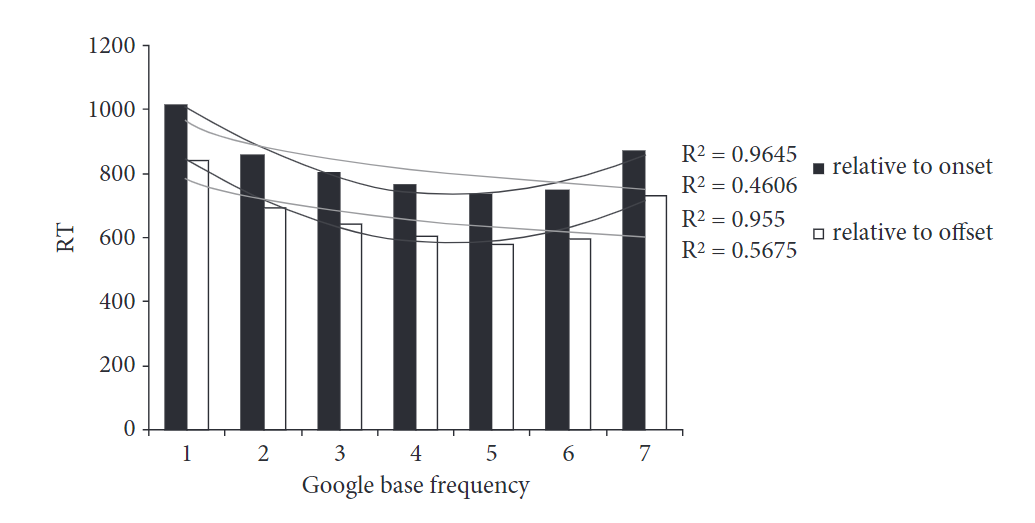
\includegraphics[keepaspectratio]{Chapters/Recognizability/Write-up/Figures/kapatsinskiradicke_graph.png}}

}

\end{figure}%

\begin{figure}[htbp]

\caption{\label{fig-lossinternalstructure}A diagram of two ways the word
\emph{pick up} could be stored. The left tree demonstrates a stored
representation of \emph{pick up}, where the internal structure is still
intact. The right tree demonstrates a holistically stored unit, where
there is a loss of internal structure. Note that both of these are
stored structures, as opposed to a compositional representation of
\emph{pick up} which would be comprised of the individual
representations \emph{pick} and \emph{up}.}

\centering{

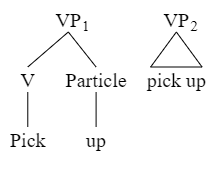
\includegraphics[width=1.13542in,height=\textheight,keepaspectratio]{Chapters/Recognizability/Write-up/Figures/syntax_tree.png}

}

\end{figure}%

It's worth noting that in the case of phrasal verbs like \emph{pick up},
it can't be the case that the entire internal representation is lost
because it is possible to syntactically alternate it (e.g., \emph{pick
up the cup} vs \emph{pick the cup up}). However, it is possible that
semantic or lemma information is lost in the holistic representation.
That is, it is possible that syntactic and/or morphological information
may be preserved even if semantic or lemma information is lost. In other
words, loss of internal representation may happen at different levels as
opposed to being an all-or-nothing process.

\subsection{Present Study}\label{present-study}

The present study examines the factors that drive storage and the
representations of stored items by extending Kapatsinski \& Radicke
(\citeproc{ref-kapatsinskiFrequencyEmergencePrefabs2009}{2009}) to look
at the effects of both frequency, predictability, and their interaction
on the processing of V+\emph{up} phrases. Similar to Kapatsinski \&
Radicke (\citeproc{ref-kapatsinskiFrequencyEmergencePrefabs2009}{2009})
, participants are tasked with pressing a button once they hear the
segment \emph{up} (which in our study occurs either as a particle within
verb phrases, e.g., \emph{pick up}, or part of a word, e.g.,
\emph{puppet}), but in our case the stimuli varied in frequency,
predictability, and whether they were a phrasal verb or not. Since both
frequency and predictability effects are rather robust in the
literature, we should at the very least see a negative correlation
between frequency and predictability and recognition time (up to perhaps
a certain point, where recognition time may increase). Further, if
predictability is not a driving factor of storage, we should see an
increase in recognition times for only the most \emph{frequent} phrases.
On the other hand, if predictability does drive storage, we may see an
increase in reaction time for both frequent and predictable phrases.

\section{Methods}\label{methods-4}

\subsection{Participants}\label{participants-4}

Participants were recruited through the University of California, Davis
Linguistics/Psychology Human Subjects Pool. 350 people participated in
this study and were compensated in the form of course credit. All
participants self-reported being native English speakers. Additionally,
44 participants were excluded due to an accuracy score below our
threshold of 70\%, leaving a total of 306 participants for the data
analysis.

\subsection{Materials}\label{materials-2}

We searched the Google \emph{n}-grams corpus
(\citeproc{ref-linSyntacticAnnotationsGoogle2012}{Lin et al., 2012}) for
the most predictable and the highest frequency phrases that matched our
criteria of containing a verb immediately followed by the word
\emph{up}. We operationalized predictability as the odds ratio of the
probability of \emph{up} occurring immediately after the verb to the
probability of any other word occurring (Equation~\ref{eq-logodds}).

\begin{equation}\phantomsection\label{eq-logodds}{
\frac{\mathrm{count(\textit{Verb+up})}}{\mathrm{count(\textit{Verb})} - \mathrm{count(\textit{Verb+up})}} 
}\end{equation}

In non-mathematical terms, the above equation quantifies how likely
\emph{up} is to follow after the verb relative to every other word that
could follow. For example, the odds ratio of \emph{pick up} would be the
number of times the entire verb phrase occurs -- \emph{pick up} --
divided by the number of times the verb -- \emph{pick} -- occurs without
\emph{up} following it.

For the purposes of the present study, we gathered a variety of phrases
that varied in both their predictability and frequency and their
combination. In order to do this, we extracted the 50 most frequent
Verb+\emph{up} items and the 50 most predictable ones. Next, we selected
100 more by randomly sampling from the remaining items. In order to
ensure stable predictability estimates we eliminated words that a
college-aged speaker wouldn't have heard more than 10 times.\footnote{Levy
  et al. (\citeproc{ref-levyProcessingExtraposedStructures2012}{2012})
  extrapolated that the average college-aged speaker has heard about 350
  million words in their lifetime. Thus we excluded items that had a
  frequency smaller than 10 per 350 million.} We then visually inspected
the data to confirm that our data spanned across both the frequency and
predictability continuum. This distribution is presented in
Figure~\ref{fig-stimplot}.

\begin{figure}[htbp]

\caption{\label{fig-stimplot}log-predictability by log-frequency (per
million) plot of our items.}

\centering{

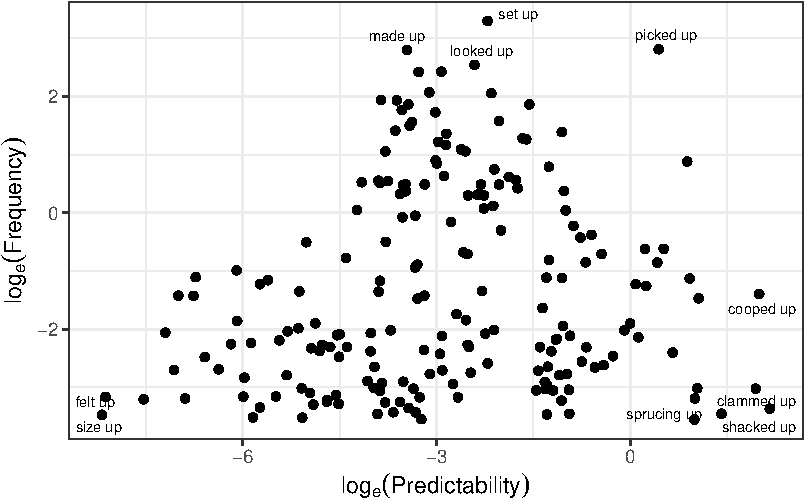
\includegraphics[width=0.8\linewidth,height=\textheight,keepaspectratio]{Chapters/Recognizability/Write-up/quarto-writeup_files/figure-pdf/fig-stimplot-1.pdf}

}

\end{figure}%

Phrasal verbs show a syntactic alternation that is not present in all
verb+\emph{up} collocations (e.g., in the example below \emph{lightened
up the room} is fine, but \emph{lightened the room up} is weird at
best). It is possible that due to this syntactic alternation, phrasal
verbs may be stored regardless of frequency and predictability. This is
because in order to properly use phrasal verbs, a speaker must be aware
of the syntactic alternation, which can't simply be predicted
compositionally (e.g., some V+\emph{up} phrases are phrasal verbs, while
other V+\emph{up} phrases are not phrasal verbs\footnote{Note that this
  largely correlates with whether the verb is transitive or not.}).
Thus, we additionally coded our stimuli for whether they were phrasal
verbs or not. This coding was done based on whether they could
syntactically alternate between having the noun within the verb phrase
and having the noun immediately after the verb phrase. For example,
since both \emph{pick the cat up} and \emph{pick up the cat} are
grammatical, \emph{pick up} was classified as a phrasal verb. Each item
was checked by two of the authors. Disagreement was easily resolved by
discussion and an agreement was reached for every item.

\begin{exe} 
\ex
  \begin{xlist}
    \ex The student lightened up the room. \\
    \ex ??The student lightened the room up. \\
  \end{xlist}
\end{exe}

We also searched the same corpus for words that contained the segment
\emph{up} (e.g., \emph{cupcake}). In order to gather a subset of words
that roughly matches the frequency range of our experimental stimuli, we
extracted the 50 most frequent words, then sampled from the rest of the
dataset to gather an additional 100 words. These 350 items together
comprise our stimuli.

For each item, we constructed two sentences: one sentence which
contained \emph{up}, and one sentence that was identical except that it
didn't include the segment \emph{up.} For words, the entire word was
replaced. For phrases, \emph{up} was simply deleted if possible (e.g.,
\emph{clean up} replaced with \emph{clean}). If this resulted in an
awkward sentence, the entire phrase was replaced. An example is given
below.

\begin{exe} 
\ex
  \begin{xlist}
    \ex He picked up the phone and answered the call. \\
    \ex He grabbed the phone and answered the call. \\
  \end{xlist}
\end{exe}

In summary, our stimuli were comprised of 200 Verb+\emph{up} phrases
that varied in both frequency and predictability, 150 words that
contained \emph{up}, and 350 filler sentences which were matched with
our experimental sentences with the exception of having \emph{up}
replaced.

After creating the sentences, a native English speaker then recorded
each sentence in a random order to minimize any list effect. We
subsequently equalized the amplitude such that every sentence was
roughly the same loudness.

\subsection{Procedure}\label{procedure-3}

Participants were presented with audio sentences via Pavlovia
(\url{https://pavlovia.org/}), a website for presenting PsychoPy
experiments (\citeproc{ref-peirce2019psychopy2}{Peirce et al., 2019}).
Each participant was presented with 3 practice trials and then 350
sentences. While we had a total of 700 sentences, participants didn't
see both the filler and experimental sentence for the same item, thus
they only saw half of the stimuli. The order of the sentences was random
and exactly half of the sentences contained the target segment (to avoid
biasing the participants towards a specific response). Participants were
instructed to press a key as soon as they heard the segment \emph{up},
or to press a separate key at the end of the sentence if they did not
hear the target segment in the sentence. We then recorded their reaction
time of the button press. The experiment took approximately 40 minutes.

\section{Results}\label{results-4}

The data\footnote{The stimuli, data, and analyses scripts can all be
  found freely available here:
  \url{https://github.com/znhoughton/Recognizability-Experiment}} was
analyzed using General Additive Mixed models, as implemented in the
\emph{mgcv} package (\citeproc{ref-wood2011fast}{Wood, 2011}) within the
R programming environment (\citeproc{ref-Rpackage}{R Core Team, 2022}).
General Additive Mixed Models are models that allow us to model our
outcome variable as a combination of the predictors. GAMMs differ from
generalized linear regression models in that they allow the predictors
to be modeled as non-linear functions, similar to polynomial regression.
Specifically, in a Generalized Additive Mixed Model, beta-coefficients
are replaced with a smooth function, which is a combination of splines.
The more splines that we include, the more wiggly our line will be. In
order to avoid overfitting, GAMMs also include a penalty term,
\(\lambda\), which can be modified to penalize more wiggly lines that
aren't justified by the data. While the predictors are allowed to vary
non-linearly, the linking function in our case was linear (i.e.,
response time varied linearly with the spline functions). Our decision
to use GAMMs was driven by our hypothesis that recognition times may
vary non-linearly as a function of frequency and/or predictability (as
suggested by
\citeproc{ref-kapatsinskiFrequencyEmergencePrefabs2009}{Kapatsinski \&
Radicke, 2009}).

For all of our models, the dependent variable was the time it took for
participants to react to the onset of the target segment in experimental
sentences/sentences containing \emph{up} (i.e., the time it took
participants to press the button after hearing \emph{up}).

In order to visualize the surface of the interaction effect between
frequency and predictability, we first ran a model with our independent
variable as the interaction between log-predictability and
log-frequency, which was allowed to vary non-linearly, and duration of
the segment, which was not allowed to vary non-linearly. Additionally,
we also included random intercepts for participant, trial, and item, as
well as random by-participant slopes for predictability, frequency,
their interaction, and trial. All our random-effects were allowed to be
wiggly (non-linear). Our model formula is included below in
Equation~\ref{eq-gamminteraction}. This model allows us to visualize the
surface of the interaction effect. Note that in GAMMs, the syntax
\texttt{ti()} is used to model the interaction effects since it produces
a tensor product interaction from which the main-effects have been
excluded. On the other hand \texttt{te()} models the full tensor product
smooth without the main-effects excluded. Thus when modeling the
main-effects with the interaction effect we use \texttt{ti()} and when
modeling the surface (that is, without separating the main-effects from
the interaction) we use \texttt{te()}.

\begin{equation}\phantomsection\label{eq-gamminteraction}{
\begin{aligned}log(RT) & \sim te(Predictability, Frequency) + Duration + s(participant, bs = \text{`}re\text{'}) + s(Item, bs = \text{`}re\text{'}) \\& + s(trial, bs = \text{`}re\text{'}) + s(Predictability, Frequency, participant, bs = \text{`}re\text{'}) \end{aligned}
}\end{equation}

The results of this model are presented in Table~\ref{tbl-gamModelTab}
and visualized in Figure~\ref{fig-gam2dplot1}. We found no significant
effect of the tensor product smooth.\footnote{We also examined the
  interaction between frequency and predictability on accuracy (whether
  they correctly responded to whether \emph{up} was present in the
  sentence) and similarly found no significant effect.} Although the
tensor product smooth for the interaction effect was not significant,
it's possible that phrasal verbs and non-phrasal verbs behave
differently and that could be why we don't see an interaction effect. As
such, we ran an additional model examining whether the interaction
effect was different for phrasal verbs versus non-phrasal verbs. The
results for this model are reported in
Table~\ref{tbl-gamModelPhrasalNonPhrasalTab}. The results suggest that
there is no difference between phrasal and non-phrasal verbs.

It is also possible that despite a lack of an interaction effect, that
frequency or predictability independently affect recognition times.
Thus, we ran an additional Generalized Additive Model with
log-frequency, log-predictability, and the interaction between
log-frequency and log-predictability as fixed-effects that could vary
non-linearly. Similar to before, duration of the segment was also
modeled as a fixed-effect that could not vary non-linearly. The
random-effects structure for this model was identical to the previous
two models. The model syntax is included below in
Equation~\ref{eq-gammFull}:

\begin{equation}\phantomsection\label{eq-gammFull}{
\begin{aligned}log(RT) & \sim ti(Predictability) + ti(Frequency) + ti(Predictability, Frequency) + Duration \\ & + s(participant, bs = \text{`}re\text{'}) + s(Item, bs = \text{`}re\text{'})  + s(trial, bs = \text{`}re\text{'}) \\ & + s(Predictability, Frequency, Trial, Participant, bs = \text{`}re\text{'}) \end{aligned}
}\end{equation}

Our results are presented in Table~\ref{tbl-gamModelInterTab};
Equation~\ref{eq-gammFull} and visualized in
Figure~\ref{fig-gammodelinterplot}. The results demonstrated a
significant main-effect of predictability (\emph{p} \textless{} 0.05),
but no significant effect of frequency (\emph{p} = 0.327).\footnote{We
  ran a follow-up model without the interaction to determine whether
  including the interaction effect takes away our power to detect an
  effect of frequency, however the results for our main-effects are
  consistent regardless of whether we include the interaction between
  frequency and predictability in the model.}

To summarize the results of our generalized additive models, we found no
interaction effect between frequency and predictability, no main effect
of frequency, but we do find a significant main effect of
predictability.

In the Psycholinguistics literature, generalized additive mixed models
are not yet well established. Thus, we ran a follow-up Bayesian
quadratic regression model to further examine the effects of frequency
and predictability on recognition times. Since the Generalized Additive
Model suggested that there was no significant interaction between
frequency and predictability, we left out the interaction term from the
regression model. The random-effects were modeled without correlations
between them in order to allow the model to run faster.
Equation~\ref{eq-BayesianFullModelSyntax} below presents the full model
syntax:

\begin{equation}\phantomsection\label{eq-BayesianFullModelSyntax}{
\begin{aligned}
log(RT) & \sim  log(Frequency) + log(Predictability) + Duration + log(Frequency)^2  + log(Predictability)^2 \\ & + (1 + log(Frequency) + log(Predictability) + log(Frequency^2) + log(Predictability^2) \\& + Duration || Participant) + (1 || Item)
\end{aligned}
}\end{equation}

The results of this model are presented in
Table~\ref{tbl-brmsQuadraticNoInter} and visualized in
Figure~\ref{fig-FullQuadraticPlot}. Following Houghton et al.
(\citeproc{ref-houghtonTaskdependentConsequencesDisfluency2024}{2024}),
in some cases where the credible interval crosses zero, we also report
the percentage of posterior samples greater than or less than zero. For
the current model, although the credible intervals for both quadratic
terms crossed zero, nearly 97\% of the posterior samples for
predictability\(^2\) were greater than zero, and nearly 93\% of the
posterior samples for frequency\(^2\) were greater than zero. A plot of
the posterior distribution for each coefficient is presented in
Figure~\ref{fig-posteriorplotFullQuadratic}. The results suggest a
U-shaped effect of predictability and a marginal u-shaped effect of
frequency on recognition times. In other words, participants recognized
\emph{up} faster as frequency or predictability increased, except for
the most frequent or most predictable items, where participants were
slower to recognize \emph{up}.

Finally, we replicated the analyses from Kapatsinski \& Radicke
(\citeproc{ref-kapatsinskiFrequencyEmergencePrefabs2009}{2009}) using
two Bayesian quadratic regression models (implemented in \emph{brms;}
\citeproc{ref-burknerBrmsPackageBayesian2017}{Bürkner, 2017}), one which
only included frequency, and one which only included predictability. For
the frequency model, the fixed-effects were log-frequency and
log-frequency\(^2\), along with duration. The model also included random
intercepts for participant and item, and random slopes for log-frequency
by participant, duration by participant, and log-frequency\(^2\) by
participant.

The quadratic regression with predictability was identical to the
quadratic regression with frequency, except that log-frequency was
replaced with log-predictability, and log-frequency\(^2\) was replaced
with log-predictability\(^2\). The random-effects were modeled without
correlations between them for both models (this was done to allow the
model to run faster, since we collected a large amount of data).

The model syntax for both models is included below in
Equation~\ref{eq-brmsFreq} and Equation~\ref{eq-brmsPredic}:

\begin{equation}\phantomsection\label{eq-brmsFreq}{
\begin{aligned}
log(RT) & \sim log(Frequency) + Duration + log(Frequency)^2 \\ & + (1 + log(Frequency) + log(Frequency)^2 + Duration || Participant) + (1 || Item)
\end{aligned}
}\end{equation}

\begin{equation}\phantomsection\label{eq-brmsPredic}{
\begin{aligned}
log(RT) & \sim log(Predictability) + Duration + log(Predictability)^2 \\ & + (1 + log(Predictability) + log(Predictability)^2 + Duration || Participant) + (1 || Item)
\end{aligned}
}\end{equation}

The results of our first model are presented in
Table~\ref{tbl-brmsFreq}. While the credible interval for
log(frequency)\(^2\) crosses zero, over 95\% of the posterior samples
were greater than zero, suggesting an effect of frequency\(^2\) on
recognition times. A visualization of the model predictions is presented
in Figure~\ref{fig-FreqOnlyPlot} and a visualization of the posterior
distribution is presented in Figure~\ref{fig-FreqOnlyBetaPlot}.

The results of our second model are presented in
Table~\ref{tbl-brmsPredic}. While the credible interval for
log(predictability)\(^2\) crosses zero, over 96\% of the posterior
samples were greater than zero, suggesting a meaningful effect. A
visualization of the model predictions is included in
Figure~\ref{fig-PredicOnlyPlot} and a visualization of the posterior
distribution is presented in Figure~\ref{fig-PredicOnlyBetaPlot}.

In summary, our results suggest that when considered independently,
there appears to be a U-shaped effect for both frequency and
predictability. The effect for frequency is not as reliably detected
when predictability is also accounted for in our models, however we do
find weak evidence for it. We do not find strong evidence for an
interaction between frequency and predictability but it is possible that
our study simply does not have the power to detect an interaction
effect.

\begin{table}

\caption{\label{tbl-gamModelTab}Model results for the generalized
Additive Mixed Model cotanining only the interaction between frequency
and predictability.}

\centering{

\begin{tabular}{lrrrl}
\toprule
  & edf & Ref.df & F & p-value\\
\midrule
te(log-predictability, log-frequency) & 5.59 & 5.73 & 1.86 & 0.090\\
s(trial) & 0.99 & 1.00 & 115.38 & <0.001\\
s(participant) & 296.00 & 305.00 & 39.74 & <0.001\\
s(item) & 175.44 & 195.00 & 10.68 & <0.001\\
s(log-predictability, log-frequency, trial, participant) & 43.00 & 306.00 & 0.46 & 0.100\\
\bottomrule
\end{tabular}

}

\end{table}%

\begin{table}

\caption{\label{tbl-gamModelPhrasalNonPhrasalTab}Model results for the
Generalized Additive Mixed Model cotaining the interaction between
frequency and predictability for phrasal vs nonphrasal verbs.}

\centering{

\begin{tabular}{lrrrl}
\toprule
  & edf & Ref.df & F & p-value\\
\midrule
te(log-predictability, log-frequency):Nonphrasal & 3.93 & 3.98 & 1.46 & 0.210\\
te(log-predictability, log-frequency):Phrasal & 4.07 & 4.12 & 1.27 & 0.240\\
s(trial) & 0.99 & 1.00 & 115.65 & <0.001\\
s(participant) & 295.99 & 305.00 & 39.83 & <0.001\\
s(item) & 172.59 & 191.00 & 10.94 & <0.001\\
\addlinespace
s(log-predictability, log-frequency, trial, participant) & 42.97 & 306.00 & 0.46 & 0.100\\
\bottomrule
\end{tabular}

}

\end{table}%

\begin{table}

\caption{\label{tbl-gamModelInterTab}Model results for the Generalized
Additive Mixed Model cotaining Frequency, Predictability, and the
interaction between them.}

\centering{

\begin{tabular}{lrrrl}
\toprule
  & edf & Ref.df & F & p-value\\
\midrule
ti(log-frequency) & 2.16 & 2.20 & 1.73 & 0.270\\
ti(log-predictability) & 1.97 & 2.01 & 4.10 & 0.020\\
ti(log-frequency, log-predictability) & 1.00 & 1.00 & 0.89 & 0.350\\
s(participant) & 296.33 & 305.00 & 37.72 & <0.001\\
s(item) & 175.70 & 195.00 & 10.76 & <0.001\\
\addlinespace
s(log-predictability, log-frequency, participant) & 0.17 & 305.00 & 0.00 & 0.600\\
\bottomrule
\end{tabular}

}

\end{table}%

\begin{table}

\caption{\label{tbl-brmsFreq}Results for the Bayesian quadratic
regression model containing only frequency and frequency\(^2\).}

\centering{

\begin{tabular}{lllllr}
\toprule
  & Estimate & Est.Error & Q2.5 & Q97.5 & \% Samples > 0\\
\midrule
Intercept & -0.102 & 0.025 & -0.150 & -0.054 & 0.000\\
log-frequency & 0.016 & 0.011 & -0.005 & 0.038 & 93.310\\
Duration & -0.084 & 0.098 & -0.274 & 0.108 & 19.355\\
log-frequency\textasciicircum{}2 & 0.006 & 0.004 & -0.001 & 0.013 & 95.225\\
\bottomrule
\end{tabular}

}

\end{table}%

\begin{table}

\caption{\label{tbl-brmsPredic}Results for the Bayesian quadratic
regression model containing only predidctability and
predictability\(^2\).}

\centering{

\begin{tabular}{lllllr}
\toprule
  & Estimate & Est.Error & Q2.5 & Q97.5 & \% Samples > 0\\
\midrule
Intercept & -0.110 & 0.027 & -0.163 & -0.058 & 0.0000\\
log-predictability & 0.008 & 0.011 & -0.014 & 0.029 & 75.7350\\
Duration & -0.089 & 0.098 & -0.280 & 0.102 & 18.4225\\
log-predictability\textasciicircum{}2 & 0.003 & 0.002 & -0.000 & 0.006 & 96.0975\\
\bottomrule
\end{tabular}

}

\end{table}%

\begin{table}

\caption{\label{tbl-brmsQuadraticNoInter}Model results for the Bayesian
quadratic regression model containing fixed-effects for frequency,
predictability, and their quadratics.}

\centering{

\begin{tabular}{lllllr}
\toprule
  & Estimate & Est.Error & Q2.5 & Q97.5 & \% Samples > 0\\
\midrule
Intercept & -0.102 & 0.029 & -0.161 & -0.046 & 0.02625\\
log-frequency & 0.019 & 0.011 & -0.002 & 0.041 & 96.15625\\
log-predictability & 0.009 & 0.011 & -0.013 & 0.032 & 78.99750\\
duration & -0.135 & 0.098 & -0.328 & 0.057 & 8.27125\\
log-predictability\textasciicircum{}2 & 0.003 & 0.002 & -0.000 & 0.007 & 96.88125\\
\addlinespace
log-frequency\textasciicircum{}2 & 0.005 & 0.004 & -0.002 & 0.012 & 92.94375\\
\bottomrule
\end{tabular}

}

\end{table}%

\begin{figure}[htbp]

\caption{\label{fig-FreqOnlyBetaPlot}Plot of the posterior distribution
for the beta value of each fixed-effect in our frequency-only quadratic
regression model. The y-axis contains the different fixed-effects and
the x-axis contains the posterior distribution of beta values for the
corresponding fixed-effect.}

\centering{

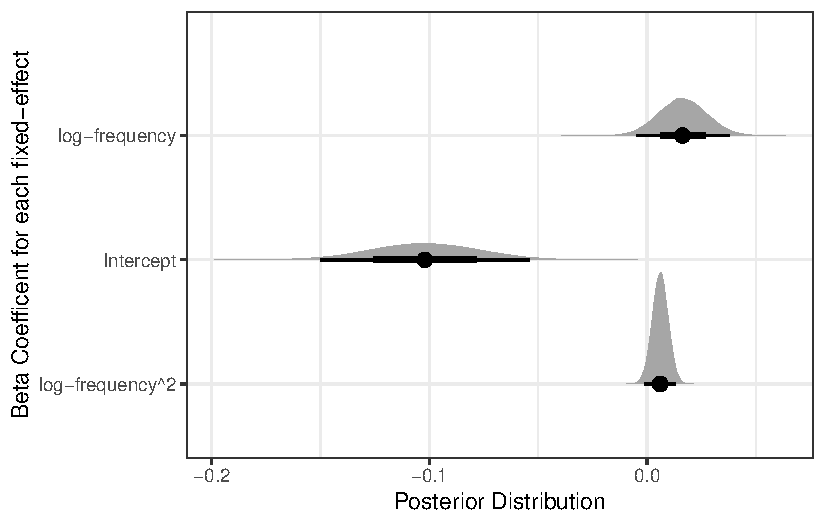
\includegraphics[width=0.8\linewidth,height=\textheight,keepaspectratio]{Chapters/Recognizability/Write-up/quarto-writeup_files/figure-pdf/fig-FreqOnlyBetaPlot-1.pdf}

}

\end{figure}%

\begin{figure}[htbp]

\caption{\label{fig-PredicOnlyBetaPlot}Plot of the posterior
distribution for the beta value of each fixed-effect in our
predictability-only quadratic regression model. The y-axis contains the
different fixed-effects and the x-axis contains the posterior
distribution of beta values for the corresponding fixed-effect.}

\centering{

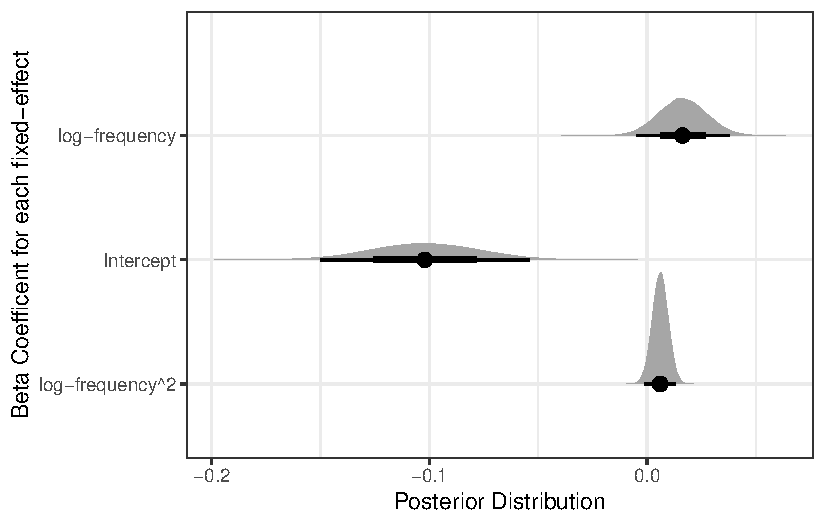
\includegraphics[width=0.8\linewidth,height=\textheight,keepaspectratio]{Chapters/Recognizability/Write-up/quarto-writeup_files/figure-pdf/fig-PredicOnlyBetaPlot-1.pdf}

}

\end{figure}%

\begin{figure}[htbp]

\caption{\label{fig-FreqOnlyPlot}Model predictions for the effects of
frequency on reaction times for the frequency-only Bayesian quadratic
model.}

\centering{

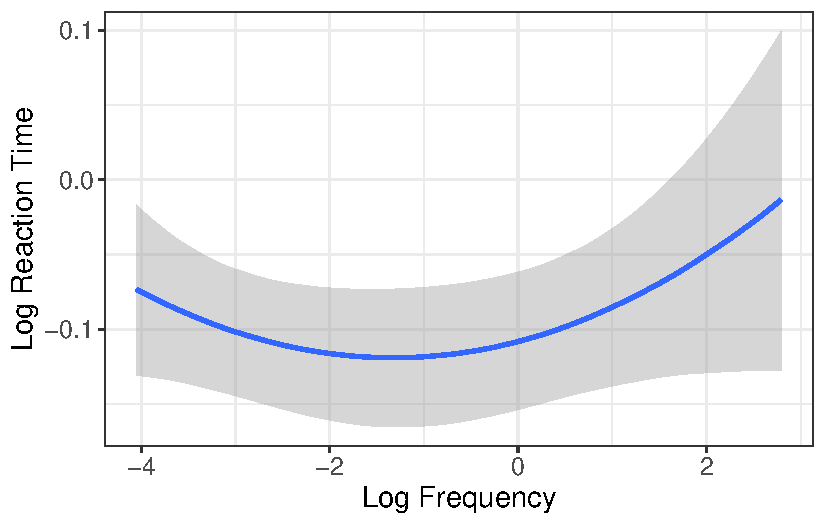
\includegraphics[width=0.6\linewidth,height=\textheight,keepaspectratio]{Chapters/Recognizability/Write-up/quarto-writeup_files/figure-pdf/fig-FreqOnlyPlot-1.pdf}

}

\end{figure}%

\begin{figure}[htbp]

\caption{\label{fig-PredicOnlyPlot}Model predictions for the effect of
predictability on reaction times for the predictability-only models.}

\centering{

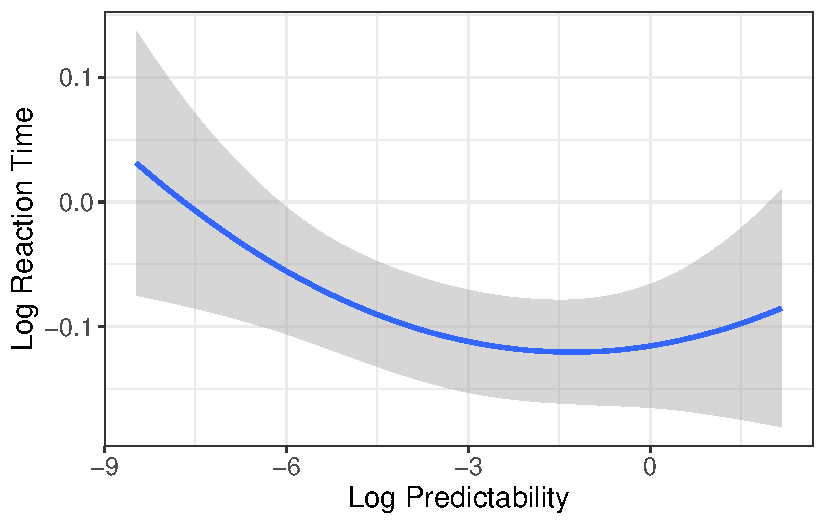
\includegraphics[width=0.6\linewidth,height=\textheight,keepaspectratio]{Chapters/Recognizability/Write-up/quarto-writeup_files/figure-pdf/fig-PredicOnlyPlot-1.pdf}

}

\end{figure}%

\begin{figure}[htbp]

\caption{\label{fig-gam2dplot1}Plot of the interaction effect between
predictability and frequency of our GAM model containing only the
interaction between frequency and predictability. The brightness of the
coloration denotes the strength of the effect at the point in the graph.
Brighter colors denote longer reaction times.}

\centering{

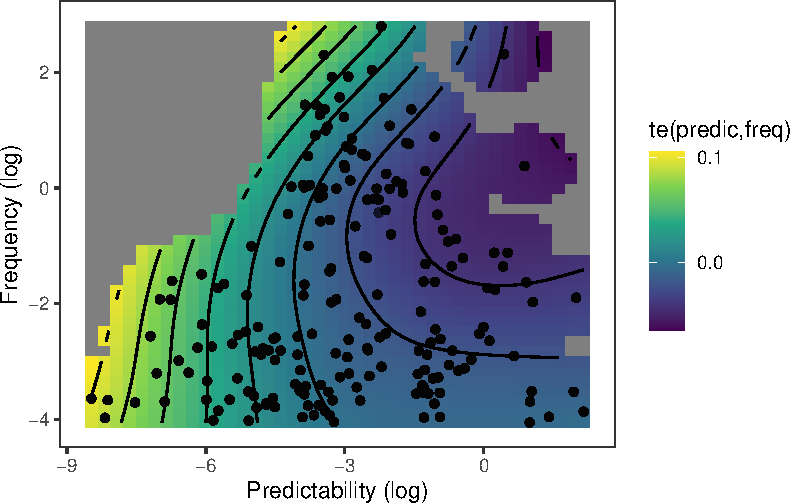
\includegraphics[width=0.8\linewidth,height=\textheight,keepaspectratio]{Chapters/Recognizability/Write-up/quarto-writeup_files/figure-pdf/fig-gam2dplot1-1.pdf}

}

\end{figure}%

\begin{figure}[htbp]

\caption{\label{fig-gammodelinterplot}Plot of our GAM model's predicted
effect of log(predictability) on recognition time.}

\centering{

\pandocbounded{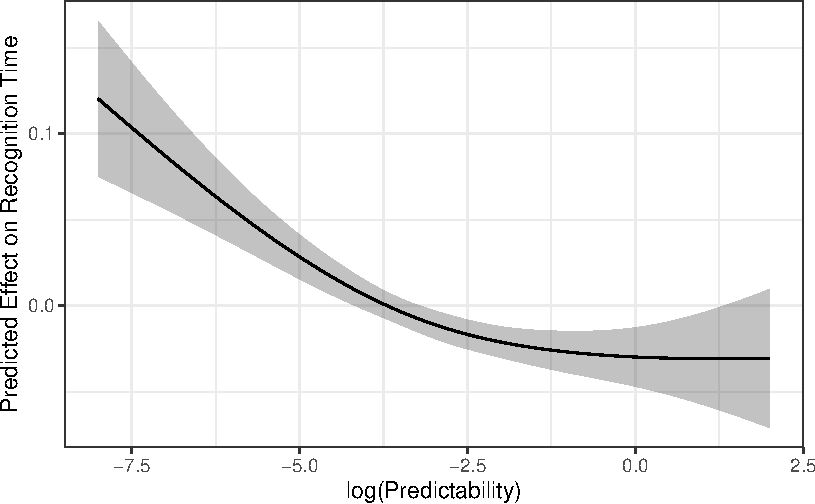
\includegraphics[keepaspectratio]{Chapters/Recognizability/Write-up/quarto-writeup_files/figure-pdf/fig-gammodelinterplot-1.pdf}}

}

\end{figure}%

\begin{figure}[htbp]

\caption{\label{fig-posteriorplotFullQuadratic}Plot of the posterior
distribution for the beta value of each fixed-effect in our Bayesian
quadratic regression model. The y-axis contains the different
fixed-effects and the x-axis contains the posterior distribution of beta
values for the corresponding fixed-effect.}

\centering{

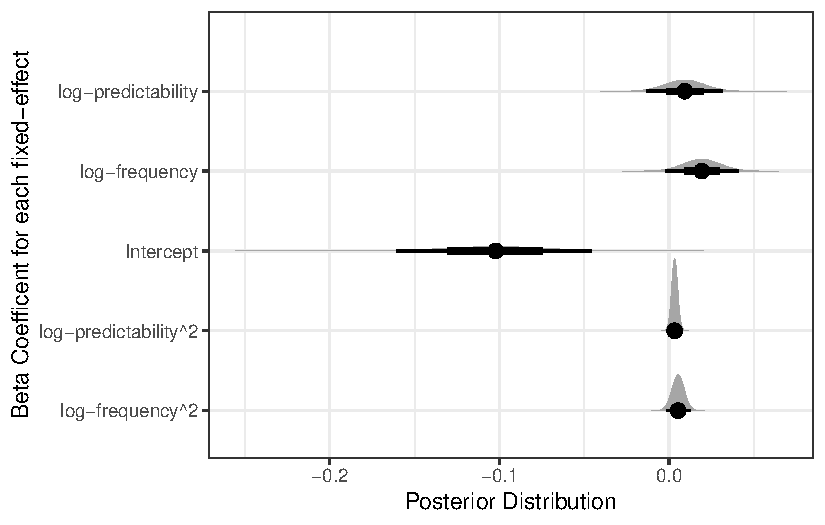
\includegraphics[width=0.8\linewidth,height=\textheight,keepaspectratio]{Chapters/Recognizability/Write-up/quarto-writeup_files/figure-pdf/fig-posteriorplotFullQuadratic-1.pdf}

}

\end{figure}%

\begin{figure}[htbp]

\caption{\label{fig-FullQuadraticPlot}Visualization of the model results
from Table~\ref{tbl-brmsQuadraticNoInter} for frequency (top) and
predictability (bottom). Frequencies are per million.}

\centering{

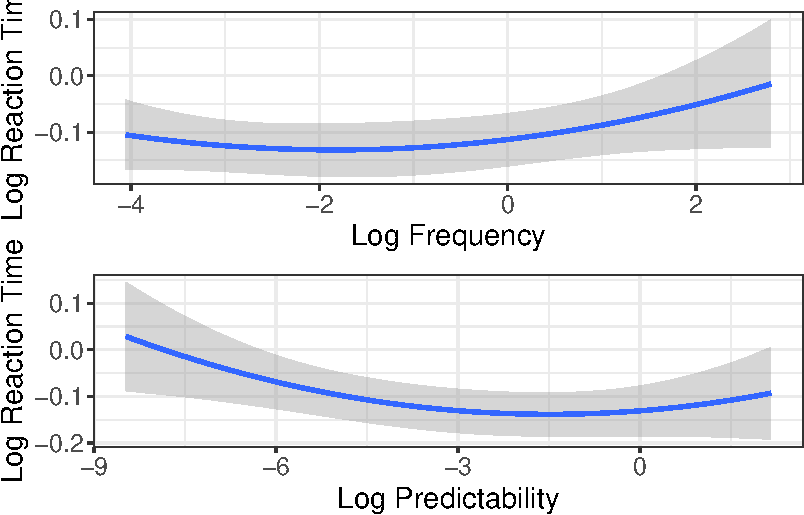
\includegraphics[width=0.8\linewidth,height=\textheight,keepaspectratio]{Chapters/Recognizability/Write-up/quarto-writeup_files/figure-pdf/fig-FullQuadraticPlot-1.pdf}

}

\end{figure}%

\section{Discussion}\label{discussion-4}

The present study examined the effects of frequency and predictability
on the recognizability of the particle \emph{up} in English phrasal
verbs. We found a U-shaped effect for both frequency and predictability
on recognizability: as frequency and predictability increased, people
were faster at recognizing \emph{up}, until reaching the highest
frequency/most predictable items, where people were slower.
Additionally, we also found no meaningful differences between phrasal
verbs (e.g., \emph{pick up}) and non-phrasal verbs (e.g., \emph{stir
up}), suggesting that this slowdown is due to statistical properties of
the language as opposed to syntactic properties.

There are three possible accounts for the slowdown we see for the
highest frequency or predictability items. First, it's possible that
people are attending less to \emph{up} or even skipping it in high
frequency and high predictability phrases. This account, unlike the
other accounts that we'll discuss, does not explicitly require the high
frequency and high predictability phrases to be stored. Instead, the
listener may be able to process the meaning of the phrase fast enough
that they don't need to wait to hear the entire phrase. For example,
it's possible that for high-frequency and high-predictability items,
when accessing the first word, e.g., \emph{pick}, the listener accesses
the representation of the entire phrase --- either a holistic
representation or a compositional representation --- immediately, before
even hearing \emph{up}. The listener can then continue to process the
next words (skipping over \emph{up}). Since the task is to respond when
they hear \emph{up}, the delay in reaction time may be because they're
not accessing the phonological representation of \emph{up}. Instead,
they may access the semantic representation of the phrase without
initially accessing the phonological representation of \emph{up} and go
on to recover the phonological representation from the semantic
representation of the phrase, causing a delay in recognition time.
Indeed, this possibility was suggested by Healy
(\citeproc{ref-healyDetectionErrorsWord1976}{1976}), who suggested that
in reading once people process the meaning of a word, they move on to
the next word regardless of whether they have processed each individual
letter. This account doesn't explicitly require \emph{pick up} to be
stored holistically since a listener could hear \emph{pick}, predict
\emph{up}, and compose the meaning \emph{pick up} despite having not
heard \emph{up}. However, it also isn't incompatible with a storage
account, since the listener might hear \emph{pick,} predict \emph{up},
and then accesses a stored holistic representation of \emph{pick up}. In
other words, if listeners are attending less to \emph{up}, then it's
unclear whether the listeners are accessing a representation formed by a
compositional process (i.e., accessing \emph{pick,} predicting
\emph{up,} and composing \emph{pick up}) or simply retrieving a stored
form from memory (accessing a holistic representation \emph{pick up}).

The next two accounts all require the high-frequency and
high-predictability items to be stored holistically, but vary with
respect to whether the holistically stored representations retain their
internal structure.

It is possible that the slowdown for the high frequency and high
predictability items is due to competition between an additional
representation. This competition can either be between a holistic
representation that has internal structure and a compositional
representation, or between a holistic representation that does not have
internal structure and the compositional representation. Compositional
representation here refers to a representation that is formed by
accessing individual forms (e.g., \emph{pick} and \emph{up}) and
combining them via some generative process. High-frequency and
high-predictability items may develop a holistic representation separate
from the compositional representation and this additional representation
may compete with the compositional representation causing the slowdown.
This account doesn't necessarily need to involve a loss of internal
structure because simply having an additional representation to compete
with can result in a slowdown, however it also not incompatible with an
account where the holistic representation has lost some of its internal
structure. These two possibilities both account for the slowdown at the
highest frequency and highest predictability items.

To break it down further, there is a good deal of evidence that
different mental representations compete for recognition
(\citeproc{ref-oppenheimLexicalCompetitionDemand2019}{Oppenheim \&
Balatsou, 2019}; c.f.
\citeproc{ref-staubInfluenceClozeProbability2015}{Staub et al., 2015}).
A representation is selected once it receives sufficiently more
activation than its competitors
(\citeproc{ref-mcclellandInteractiveActivationModel1981}{McClelland \&
Rumelhart, 1981}). For example, in picture-naming tasks in which
participants are tasked with naming a picture while confronted with a
distractor word, participants are generally slower to produce the
intended word when the distractor word is semantically related to the
picture
(\citeproc{ref-mcclellandInteractiveActivationModel1981}{McClelland \&
Rumelhart, 1981};
\citeproc{ref-schriefersExploringTimeCourse1990}{Schriefers et al.,
1990};
\citeproc{ref-starreveldSemanticInterferenceOrthographic1995}{Starreveld
\& La Heij, 1995}). This effect is not restricted to production as we
see similar competition effects in comprehension as well. For example,
Magnuson et al.
(\citeproc{ref-magnusonDynamicsLexicalCompetition2007}{2007}) examined
the role of competition in word recognition using a visual world
paradigm, where participants saw words on a screen and were instructed
to select the word that they heard. To measure word-recognition, an
eye-tracker was used to track pupil fixations. In each of the trials
there was a single distractor image. They found that words with low
cohort density (i.e., words that have fewer phonological competitors)
showed a larger proportion of target to nontarget fixations. That is,
participants looked the distractor image less relative to the target
word when the word had fewer competitors. Given the inhibitory effects
of competition, it is possible that the delay in reaction time for
\emph{up} in high-frequency and predictability phrases may be a
consequence of an additional representation competing with the
compositional representation. However, there is also evidence that
competition has no effect on comprehension
(\citeproc{ref-staubInfluenceClozeProbability2015}{Staub et al., 2015}).
Using reaction time data from a cloze completion task, Staub et al.
(\citeproc{ref-staubInfluenceClozeProbability2015}{2015}) demonstrated
that a RACE model with neither facilitation nor inhibition between
competitors can account for the data. Thus the evidence for competition
effects in comprehension is mixed. Note that this account is agnostic
about whether the holistic representation has lost its internal
structure or not: simply having an additional representation to compete
with can cause the slowdown.

Lastly it is possible that rather than being driven by competition,
listeners are simply accessing a holistically stored representation of
the phrase that lacks internal structure. This interpretation seems
quite likely given that we see a U-shaped effect in both phrasal (e.g.,
\emph{pick up}) and non-phrasal verbs (e.g., \emph{stir up}). Phrasal
verbs have a syntactic alternation that may lead to all of them being
stored, regardless of whether they are frequent/predictable or not. For
example, In a corpus study, Hampe
(\citeproc{ref-hampeTransitivePhrasalVerbs2012}{2012}) argued that
\emph{Verb-Object-Particle} constructions and
\emph{Verb-Particle-Object} constructions are two distinct
constructions.\footnote{However, the same study also makes the claim
  that these templates are different from more lexically specific
  constructions, thus it is unclear in what ways these templates may
  pattern similarly to holistically stored lexical items.} If the
increase in reaction time is simply due to competition between the
holistically stored representation and the individual word-level
representations, then if all phrasal verbs are stored we would expect
all of the phrasal verbs to be recognized more slowly. This is because
all of the phrasal verbs, regardless of frequency, would have an
additional representation that would compete for activation. However, we
only see a slowdown for the most frequent or most predictable phrases,
suggesting that storage alone isn't driving the effect. Instead, it is
the combination of storage and usage that leads to loss of internal
representation.

One explanation for why high frequency and high predictability items may
not have an intact internal representation is that the internal
structure for those items may never have been learned to begin with.
Children are experts at statistical learning and use transitional
probabilities to divide the continuous speech stream
(\citeproc{ref-saffranStatisticalLearning8MonthOld1996}{Saffran et al.,
1996}). High predictability phrases in the present study, by definition,
have higher transitional probabilities between words. Thus if children
are relying on transitional probabilities to separate speech into
individual words, the individual words in the most predictable phrases
may not be separated out of the speech stream initially.

Further, many high-frequency (e.g., \emph{set up}) and
high-predictability (e.g., \emph{conjure up}) phrases have semantically
vague relationships that might make it difficult to split them up on a
semantic basis. It seems plausible then that maybe these phrases weren't
learned as being composed of individual words initially and thus the
internal structure for the holistically stored items may not have been
learned. The example, \emph{trick or treat}, is a prime example of a
phrase that does not seem to have a clear semantic relationship between
the phrase and its component parts.

On the other hand, the internal structure may have been lost over time.
For example, Harmon \& Kapatsinski
(\citeproc{ref-harmonPuttingOldTools2017}{2017}) demonstrated that as
learners repeatedly experience a form with a specific meaning, they
become more likely to use that form to express novel meanings in
production (resulting in semantic extension). It is possible that this
accessibility effect similarly drives a loss of internal structure: As a
phrase becomes more semantically extended, the internal structure may be
lost over time. That is, as a phrase such as \emph{pick up} becomes
extended to express novel meanings such as \emph{continue} (``Let's pick
up from where we last left off''), the relationship between the phrase
and its internal pieces (e.g., the relationship between \emph{pick up}
and the individual words \emph{pick} and \emph{up}) becomes less
transparent, and the learner may slowly unlearn this relationship as it
becomes less useful.

In summary, our results suggest that both frequency and predictability
may drive the holistic storage of phrasal verbs, and these holistically
stored items may compete with their component parts during lexical
access. However, future work is still needed to confirm whether the
slowdown for the highest frequency and highest predictability items is
indeed due to a stored holistic representation or if it's due to
shallower attention mechanisms.

\bookmarksetup{startatroot}

\chapter*{References}\label{references}
\addcontentsline{toc}{chapter}{References}

\markboth{References}{References}

\begingroup
\raggedright

\phantomsection\label{refs}
\begin{CSLReferences}{1}{0}
\bibitem[\citeproctext]{ref-al-selwiLSTMInefficiencyLongterm2023}
Al-Selwi, S. M., Hassan, M. F., Abdulkadir, S. J., \& Muneer, A. (2023).
LSTM inefficiency in long-term dependencies regression problems.
\emph{Journal of Advanced Research in Applied Sciences and Engineering
Technology}, \emph{30}(3), 1631.
\url{https://www.researchgate.net/profile/Amgad-Muneer-2/publication/370769893_LSTM_Inefficiency_in_Long-Term_Dependencies_Regression_Problems/links/64624134f43b8a29ba525b9b/LSTM-Inefficiency-in-Long-Term-Dependencies-Regression-Problems.pdf}

\bibitem[\citeproctext]{ref-ambridgeStoredAbstractionsRadical2020}
Ambridge, B. (2020). Against stored abstractions: A radical exemplar
model of language acquisition. \emph{First Language}, \emph{40}(5-6),
509--559. \url{https://doi.org/10.1177/0142723719869731}

\bibitem[\citeproctext]{ref-arnonMoreWordsFrequency2010}
Arnon, I., \& Snider, N. (2010). More than words: Frequency effects for
multi-word phrases. \emph{Journal of Memory and Language}, \emph{62}(1),
67--82. \url{https://doi.org/10.1016/j.jml.2009.09.005}

\bibitem[\citeproctext]{ref-baayenDutchInflectionRules2002}
Baayen, H., Schreuder, R., De Jong, N., \& Krott, A. (2002). \emph{Dutch
inflection: The rules that prove the exception} (S. Nooteboom, F.
Weerman, \& F. Wijnen, Eds.; Vol. 30, pp. 61--92). Springer Netherlands.
\url{http://link.springer.com/10.1007/978-94-010-0355-1_3}

\bibitem[\citeproctext]{ref-baayenAmorphousModelMorphological2011}
Baayen, R. H., Milin, P., rević, D. F., Hendrix, P., \& Marelli, M.
(2011). An amorphous model for morphological processing in visual
comprehension based on naive discriminative learning.
\emph{Psychological Review}, \emph{118}(3), 438--481.
\url{https://doi.org/10.1037/a0023851}

\bibitem[\citeproctext]{ref-bannardStoredWordSequences2008}
Bannard, C., \& Matthews, D. (2008). Stored Word Sequences in Language
Learning: The Effect of Familiarity on Children's Repetition of
Four-Word Combinations. \emph{Psychological Science}, \emph{19}(3),
241--248. \url{https://doi.org/10.1111/j.1467-9280.2008.02075.x}

\bibitem[\citeproctext]{ref-barrRandomEffectsStructure2013}
Barr, D. J., Levy, R., Scheepers, C., \& Tily, H. J. (2013). Random
effects structure for confirmatory hypothesis testing: Keep it maximal.
\emph{Journal of Memory and Language}, \emph{68}(3), 255--278.
\url{https://doi.org/10.1016/j.jml.2012.11.001}

\bibitem[\citeproctext]{ref-benderDangersStochasticParrots2021}
Bender, E. M., Gebru, T., McMillan-Major, A., \& Shmitchell, S. (2021).
\emph{FAccT '21: 2021 ACM Conference on Fairness, Accountability, and
Transparency}. 610--623. \url{https://doi.org/10.1145/3442188.3445922}

\bibitem[\citeproctext]{ref-bengioProblemLearningLongterm1993}
Bengio, Y., Frasconi, P., \& Simard, P. (1993). \emph{IEEE international
conference on neural networks}. 1183--1188 vol.3.
\url{https://doi.org/10.1109/ICNN.1993.298725}

\bibitem[\citeproctext]{ref-benorChickenEggProbabilistic2006}
Benor, S. B., \& Levy, R. (2006). The chicken or the egg? A
probabilistic analysis of english binomials. \emph{Language},
\emph{82}(2), 233--278. \url{https://doi.org/10.1353/lan.2006.0077}

\bibitem[\citeproctext]{ref-berkoChildsLearningEnglish1958}
Berko, J. (1958). The Child's Learning of English Morphology.
\emph{{\emph{WORD}}}, \emph{14}(2-3), 150--177.
\url{https://doi.org/10.1080/00437956.1958.11659661}

\bibitem[\citeproctext]{ref-boyceMazeMadeEasy2020}
Boyce, V., Futrell, R., \& Levy, R. P. (2020). Maze made easy: Better
and easier measurement of incremental processing difficulty.
\emph{Journal of Memory and Language}, \emph{111}(November 2019),
104082. \url{https://doi.org/10.1016/j.jml.2019.104082}

\bibitem[\citeproctext]{ref-burknerBrmsPackageBayesian2017}
Bürkner, P.-C. (2017). Brms: An r package for bayesian multilevel models
using stan. \emph{Journal of Statistical Software}, \emph{80}, 128.
\url{https://www.jstatsoft.org/article/view/v080i01}

\bibitem[\citeproctext]{ref-bybeeWordFrequencyContext2002}
Bybee, J. (2002). Word frequency and context of use in the lexical
diffusion of phonetically conditioned sound change. \emph{Language
Variation and Change}, \emph{14}(3), 261--290.
\url{https://doi.org/10.1017/S0954394502143018}

\bibitem[\citeproctext]{ref-bybee2003}
Bybee, J. (2003). \emph{Phonology and language use} (Vol. 94). Cambridge
University Press.

\bibitem[\citeproctext]{ref-bybee2001}
Bybee, J., \& Hopper, P. (2001). Introduction to frequency and the
emergence of linguistic structure. \emph{Typological Studies in
Language}, \emph{45}, 126.
\url{https://www.torrossa.com/gs/resourceProxy?an=5002168&publisher=FZ4850\#page=10}

\bibitem[\citeproctext]{ref-bybeeEffectUsageDegrees1999}
Bybee, J., \& Scheibman, J. (1999). The effect of usage on degrees of
constituency: The reduction of don't in english. \emph{Linguistics},
\emph{37}(4). \url{https://doi.org/10.1515/ling.37.4.575}

\bibitem[\citeproctext]{ref-chomsky1965}
Chomsky, N. (1965). \emph{Aspects of the theory of syntax special
technical report no. 11}.

\bibitem[\citeproctext]{ref-christiansenMoreWordsRole2017}
Christiansen, M. H., \& Arnon, I. (2017). More than words: The role of
multiword sequences in language learning and use. \emph{Topics in
Cognitive Science}, \emph{9}(3), 542--551.
\url{https://doi.org/10.1111/tops.12274}

\bibitem[\citeproctext]{ref-goldbergConstructionsNewTheoretical2003}
Goldberg, A. E. (2003). Constructions: A new theoretical approach to
language. \emph{Trends in Cognitive Sciences}, \emph{7}(5), 219--224.
\url{https://doi.org/10.1016/S1364-6613(03)00080-9}

\bibitem[\citeproctext]{ref-groeneveldOLMoAcceleratingScience2024}
Groeneveld, D., Beltagy, I., Walsh, P., Bhagia, A., Kinney, R., Tafjord,
O., Jha, A. H., Ivison, H., Magnusson, I., Wang, Y., et al. (2024).
Olmo: Accelerating the science of language models. \emph{arXiv Preprint
arXiv:2402.00838}.

\bibitem[\citeproctext]{ref-gulordava2018colorlessgreenrecurrent}
Gulordava, K., Bojanowski, P., Grave, E., Linzen, T., \& Baroni, M.
(n.d.). \emph{Colorless green recurrent networks dream hierarchically}.
\url{https://doi.org/10.48550/arXiv.1803.11138}

\bibitem[\citeproctext]{ref-haleyThisBERTNow2020}
Haley, C. (2020). \emph{This is a BERT. Now there are several of them.
Can they generalize to novel words?} 333341.
\url{https://aclanthology.org/2020.blackboxnlp-1.31/}

\bibitem[\citeproctext]{ref-hampeTransitivePhrasalVerbs2012}
Hampe, B. (2012). Transitive phrasal verbs in acquisition and use: A
view from construction grammar. \emph{Language Value}, \emph{4}(1),
1--32.
\url{https://raco.cat/index.php/LanguageValue/article/view/302086}

\bibitem[\citeproctext]{ref-harmonPuttingOldTools2017}
Harmon, Z., \& Kapatsinski, V. (2017). Putting old tools to novel uses:
The role of form accessibility in semantic extension. \emph{Cognitive
Psychology}, \emph{98}, 22--44.
\url{https://doi.org/10.1016/j.cogpsych.2017.08.002}

\bibitem[\citeproctext]{ref-healyDetectionErrorsWord1976}
Healy, A. F. (1976). Detection errors on the word the: Evidence for
reading units larger than letters. \emph{Journal of Experimental
Psychology: Human Perception and Performance}, \emph{2}(2), 235.
\url{https://psycnet.apa.org/journals/xhp/2/2/235/}

\bibitem[\citeproctext]{ref-hooperWordFrequencyLexical1976a}
Hooper, J. B. (1976). Word frequency in lexical diffusion and the source
of morphophonological change. \emph{Current Progress in Historical
Linguistics}, \emph{96}, 105.

\bibitem[\citeproctext]{ref-houghtonTaskdependentConsequencesDisfluency2024}
Houghton, Z., Kato, M., Baese-Berk, M., \& Vaughn, C. (2024).
Task-dependent consequences of disfluency in perception of native and
non-native speech. \emph{Applied Psycholinguistics}, 1--17.
\url{https://doi.org/10.1017/S0142716423000486}

\bibitem[\citeproctext]{ref-janssenPhraseFrequencyEffects2012}
Janssen, N., \& Barber, H. A. (2012). Phrase Frequency Effects in
Language Production. \emph{PLOS ONE}, \emph{7}(3), e33202.
\url{https://doi.org/10.1371/journal.pone.0033202}

\bibitem[\citeproctext]{ref-kapatsinski2018}
Kapatsinski, V. (2018). \emph{Changing minds changing tools: From
learning theory to language acquisition to language change}. MIT Press.

\bibitem[\citeproctext]{ref-kapatsinskiHierarchicalInferenceSound2021}
Kapatsinski, V. (2021). Hierarchical inference in sound change: Words,
sounds, and frequency of use. \emph{Frontiers in Psychology},
\emph{12}(August). \url{https://doi.org/10.3389/fpsyg.2021.652664}

\bibitem[\citeproctext]{ref-kapatsinskiFrequencyEmergencePrefabs2009}
Kapatsinski, V., \& Radicke, J. (2009). \emph{Frequency and the
emergence of prefabs: Evidence from monitoring}. \emph{January 2009},
499. \url{https://doi.org/10.1075/tsl.83.14kap}

\bibitem[\citeproctext]{ref-lasriSubjectVerbAgreement2022}
Lasri, K., Seminck, O., Lenci, A., \& Poibeau, T. (2022). Subject verb
agreement error patterns in meaningless sentences: Humans vs. BERT.
\emph{arXiv Preprint arXiv:2209.10538}.

\bibitem[\citeproctext]{ref-leeFrequencyEffectsMorphologisation2015}
Lee, O., \& Kapatsinski, V. (2015). \emph{Frequency effects in
morphologisation of korean /n/-epenthesis}. 1--23.

\bibitem[\citeproctext]{ref-levyProcessingExtraposedStructures2012}
Levy, R., Fedorenko, E., Breen, M., \& Gibson, E. (2012). The processing
of extraposed structures in english. \emph{Cognition}, \emph{122}(1),
12--36. \url{https://doi.org/10.1016/j.cognition.2011.07.012}

\bibitem[\citeproctext]{ref-liAreNeuralNetworks2021}
Li, B., \& Wisniewski, G. (2021). \emph{Are neural networks extracting
linguistic properties or memorizing training data? An observation with a
multilingual probe for predicting tense}.
\url{https://shs.hal.science/halshs-03197072/}

\bibitem[\citeproctext]{ref-liAssessingCapacityTransformer2023}
Li, B., Wisniewski, G., \& Crabbé, B. (2023). Assessing the capacity of
transformer to abstract syntactic representations: A contrastive
analysis based on long-distance agreement. \emph{Transactions of the
Association for Computational Linguistics}, \emph{11}, 18--33.
\url{https://doi.org/10.1162/tacl_a_00531}

\bibitem[\citeproctext]{ref-linSyntacticAnnotationsGoogle2012}
Lin, Y., Michel, J.-B., Lieberman, E. A., Orwant, J., Brockman, W., \&
Petrov, S. (2012). \emph{Syntactic annotations for the google books
ngram corpus}. 169174. \url{https://aclanthology.org/P12-3029.pdf}

\bibitem[\citeproctext]{ref-liuFrequencydependentRegularizationConstituent2020}
Liu, Z., \& Morgan, E. (2020). \emph{Frequency-dependent regularization
in constituent ordering preferences.}
\url{https://www.cognitivesciencesociety.org/cogsci20/papers/0751/0751.pdf}

\bibitem[\citeproctext]{ref-liuFrequencyDependentRegularizationSyntactic2021}
Liu, Z., \& Morgan, E. (2021). \emph{Frequency-dependent regularization
in syntactic constructions}. 387389.
\url{https://aclanthology.org/2021.scil-1.41.pdf}

\bibitem[\citeproctext]{ref-magnusonDynamicsLexicalCompetition2007}
Magnuson, J. S., Dixon, J. A., Tanenhaus, M. K., \& Aslin, R. N. (2007).
The Dynamics of Lexical Competition During Spoken Word Recognition.
\emph{Cognitive Science}, \emph{31}(1), 133--156.
\url{https://doi.org/10.1080/03640210709336987}

\bibitem[\citeproctext]{ref-mayeLearningPhonemesMinimal2000}
Maye, J., \& Gerken, L. (2000). \emph{Learning phonemes without minimal
pairs}. \emph{2}, 522533.
\url{https://www.academia.edu/download/68237640/Learning_Phonemes_Without_Minimal_Pairs20210721-21044-1t0fvya.pdf}

\bibitem[\citeproctext]{ref-mcclellandTRACEModelSpeech1984}
McClelland, J. L., Elman, J. L., \& LANGUAGE, C. U. S. D. L. J. C. F. R.
I. (1984). The TRACE model of speech perception. \emph{California
University San Diego, La Jolla Center for Research in Language}.
\url{https://apps.dtic.mil/sti/citations/ADA157550}

\bibitem[\citeproctext]{ref-mcclellandInteractiveActivationModel1981}
McClelland, J. L., \& Rumelhart, D. E. (1981). An interactive activation
model of context effects in letter perception: I. An account of basic
findings. \emph{Psychological Review}, \emph{88}(5), 375.
\url{https://psycnet.apa.org/record/1981-31825-001}

\bibitem[\citeproctext]{ref-mccoyHowMuchLanguage2023}
McCoy, R. T., Smolensky, P., Linzen, T., Gao, J., \& Celikyilmaz, A.
(2023). How much do language models copy from their training data?
Evaluating linguistic novelty in text generation using raven.
\emph{Transactions of the Association for Computational Linguistics},
\emph{11}, 652670.
\url{https://direct.mit.edu/tacl/article/doi/10.1162/tacl_a_00567/116616}

\bibitem[\citeproctext]{ref-mcmurrayWithincategoryVOTAffects2009}
McMurray, B., Tanenhaus, M. K., \& Aslin, R. N. (2009). Within-category
VOT affects recovery from {"}lexical{"} garden-paths: Evidence against
phoneme-level inhibition. \emph{Journal of Memory and Language},
\emph{60}(1), 65--91. \url{https://doi.org/10.1016/j.jml.2008.07.002}

\bibitem[\citeproctext]{ref-michel2011quantitativeanalysisculture}
Michel, J.-B., Shen, Y. K., Aiden, A. P., Veres, A., Gray, M. K., The
Google Books Team, Pickett, J. P., Hoiberg, D., Clancy, D., Norvig, P.,
Orwant, J., Pinker, S., Nowak, M. A., \& Aiden, E. L. (2011).
Quantitative Analysis of Culture Using Millions of Digitized Books.
\emph{Science}, \emph{331}(6014), 176--182.
\url{https://doi.org/10.1126/science.1199644}

\bibitem[\citeproctext]{ref-misraLanguageModelsLearn2024}
Misra, K., \& Mahowald, K. (2024). Language models learn rare phenomena
from less rare phenomena: The case of the missing AANNs. \emph{arXiv
Preprint arXiv:2403.19827}.

\bibitem[\citeproctext]{ref-mollicaHumansStoreMegabytes2019}
Mollica, F., \& Piantadosi, S. T. (2019). Humans store about 1.5
megabytes of information during language acquisition. \emph{Royal
Society Open Science}, \emph{6}(3), 181393.
\url{https://doi.org/10.1098/rsos.181393}

\bibitem[\citeproctext]{ref-morganModelingIdiosyncraticPreferences2015}
Morgan, E., \& Levy, R. (2015a). \emph{Modeling idiosyncratic
preferences : How generative knowledge and expression frequency jointly
determine language structure}. 1649--1654.

\bibitem[\citeproctext]{ref-morgan2015}
Morgan, E., \& Levy, R. (2015b). \emph{Modeling idiosyncratic
preferences: How generative knowledge and expression frequency jointly
determine language structure.}

\bibitem[\citeproctext]{ref-morganAbstractKnowledgeDirect2016}
Morgan, E., \& Levy, R. (2016a). Abstract knowledge versus direct
experience in processing of binomial expressions. \emph{Cognition},
\emph{157}, 384--402.
\url{https://doi.org/10.1016/j.cognition.2016.09.011}

\bibitem[\citeproctext]{ref-morganFrequencydependentRegularizationIterated2016a}
Morgan, E., \& Levy, R. (2016b). Frequency-dependent regularization in
iterated learning. \emph{The Evolution of Language: Proceedings of the
11th International Conference}.

\bibitem[\citeproctext]{ref-morgan2024}
Morgan, E., \& Levy, R. (2024). Productive knowledge and item-specific
knowledge trade off as a function of frequency in multiword expression
processing. \emph{Language}, \emph{100}(4), e195--e224.
\url{https://muse.jhu.edu/pub/24/article/947046}

\bibitem[\citeproctext]{ref-nooteboomStorageComputationLanguage2002}
Nooteboom, S., Nooteboom, S. G., Weerman, F., \& Wijnen, F. N. K.
(2002). \emph{Storage and computation in the language faculty}. Springer
Science \& Business Media.
\url{https://books.google.com/books?hl=en&lr=&id=Sa_dGP0AT-YC&oi=fnd&pg=PR7&dq=nootebom+storage+and+computation&ots=nYGC8JjkTW&sig=1RZzWemOQIzn6bmSH7NF396lKZQ}

\bibitem[\citeproctext]{ref-odonnellProductivityReuseLanguage2016}
O'Donnell, T. J. (2016). Productivity and reuse in language.
\emph{Productivity and Reuse in Language}, 1613--1618.
\url{https://doi.org/10.7551/mitpress/9780262028844.001.0001}

\bibitem[\citeproctext]{ref-odonnellFragmentGrammarsExploring2009}
O'Donnell, T. J., Tenenbaum, J. B., \& Goodman, N. D. (2009).
\emph{Fragment Grammars: Exploring Computation and Reuse in Language}.
\url{https://dspace.mit.edu/handle/1721.1/44963}

\bibitem[\citeproctext]{ref-olejarczukDistributionalLearningErrordriven2018}
Olejarczuk, P., Kapatsinski, V., \& Baayen, R. H. (2018). Distributional
learning is error-driven: The role of surprise in the acquisition of
phonetic categories. \emph{Linguistics Vanguard}, \emph{4}(s2), 1--9.
\url{https://doi.org/10.1515/lingvan-2017-0020}

\bibitem[\citeproctext]{ref-oppenheimLexicalCompetitionDemand2019}
Oppenheim, G. M., \& Balatsou, E. (2019). Lexical competition on demand.
\emph{Cognitive Neuropsychology}, \emph{36}(5-6), 216--219.
\url{https://doi.org/10.1080/02643294.2019.1580189}

\bibitem[\citeproctext]{ref-peirce2019psychopy2}
Peirce, J., Gray, J. R., Simpson, S., MacAskill, M., Höchenberger, R.,
Sogo, H., Kastman, E., \& Lindeløv, J. K. (2019). PsychoPy2: Experiments
in behavior made easy. \emph{Behavior Research Methods}, \emph{51},
195--203.

\bibitem[\citeproctext]{ref-pierrehumbertExemplarDynamicsWord2001}
Pierrehumbert, J. B. (2001). \emph{Exemplar dynamics: Word frequency,
lenition and contrast} (J. L. Bybee \& P. J. Hopper, Eds.; Vol. 45, p.
137). John Benjamins Publishing Company.
\url{https://doi.org/10.1075/tsl.45.08pie}

\bibitem[\citeproctext]{ref-pierrehumbertPhonologicalRepresentationAbstract2016}
Pierrehumbert, J. B. (2016). Phonological Representation: Beyond
Abstract Versus Episodic. \emph{Annual Review of Linguistics},
\emph{2}(Volume 2, 2016), 33--52.
\url{https://doi.org/10.1146/annurev-linguistics-030514-125050}

\bibitem[\citeproctext]{ref-pinker2002}
Pinker, S., \& Ullman, M. T. (2002). The past and future of the past
tense. \emph{Trends in Cognitive Sciences}, \emph{6}(11), 456--463.
\url{https://doi.org/10.1016/S1364-6613(02)01990-3}

\bibitem[\citeproctext]{ref-Rpackage}
R Core Team. (2022). \emph{R: A language and environment for statistical
computing}. R Foundation for Statistical Computing.
\url{https://www.R-project.org/}

\bibitem[\citeproctext]{ref-ramscarChildrenValueInformativity2013}
Ramscar, M., Dye, M., \& Klein, J. (2013). Children value informativity
over logic in word learning. \emph{Psychological Science}, \emph{24}(6),
1017--1023. \url{https://doi.org/10.1177/0956797612460691}

\bibitem[\citeproctext]{ref-saffranStatisticalLearning8MonthOld1996}
Saffran, J. R., Aslin, R. N., \& Newport, E. L. (1996). Statistical
Learning by 8-Month-Old Infants. \emph{Science}, \emph{274}(5294),
1926--1928. \url{https://doi.org/10.1126/science.274.5294.1926}

\bibitem[\citeproctext]{ref-schriefersExploringTimeCourse1990}
Schriefers, H., Meyer, A. S., \& Levelt, W. J. M. (1990). Exploring the
time course of lexical access in language production: Picture-word
interference studies. \emph{Journal of Memory and Language},
\emph{29}(1), 86--102.
\url{https://doi.org/10.1016/0749-596X(90)90011-N}

\bibitem[\citeproctext]{ref-siegelmanAdvantageStartingBig2015}
Siegelman, N., \& Arnon, I. (2015). The advantage of starting big:
Learning from unsegmented input facilitates mastery of grammatical
gender in an artificial language. \emph{Journal of Memory and Language},
\emph{85}, 60--75. \url{https://doi.org/10.1016/j.jml.2015.07.003}

\bibitem[\citeproctext]{ref-siyanova-chanturiaSeeingPhraseTime2011}
Siyanova-Chanturia, A., Conklin, K., \& Heuven, W. J. B. van. (2011).
Seeing a phrase {"} time and again{"} matters: The role of phrasal
frequency in the processing of multiword sequences. \emph{Journal of
Experimental Psychology: Learning Memory and Cognition}, \emph{37}(3),
776--784. \url{https://doi.org/10.1037/a0022531}

\bibitem[\citeproctext]{ref-smithZSFileFormat2014}
Smith, N. (2014). ZS: A file format for efficiently distributing, using,
and archiving record-oriented datasets of any size. \emph{Vorpus.Org},
\emph{270273}(270273), 1--39.

\bibitem[\citeproctext]{ref-starreveldSemanticInterferenceOrthographic1995}
Starreveld, P. A., \& La Heij, W. (1995). Semantic interference,
orthographic facilitation, and their interaction in naming tasks.
\emph{Journal of Experimental Psychology: Learning, Memory, and
Cognition}, \emph{21}(3), 686.
\url{https://psycnet.apa.org/record/1995-42762-001}

\bibitem[\citeproctext]{ref-staubInfluenceClozeProbability2015}
Staub, A., Grant, M., Astheimer, L., \& Cohen, A. (2015). The influence
of cloze probability and item constraint on cloze task response time.
\emph{Journal of Memory and Language}, \emph{82}, 1--17.
\url{https://doi.org/10.1016/j.jml.2015.02.004}

\bibitem[\citeproctext]{ref-staubTimeCoursePlausibility2007}
Staub, A., Rayner, K., Pollatsek, A., Hyönä, J., \& Majewski, H. (2007).
The time course of plausibility effects on eye movements in reading:
Evidence from noun-noun compounds. \emph{Journal of Experimental
Psychology: Learning Memory and Cognition}, \emph{33}(6), 1162--1169.
\url{https://doi.org/10.1037/0278-7393.33.6.1162}

\bibitem[\citeproctext]{ref-stembergerFrequencyLexicalStorage1986}
Stemberger, J. P., \& MacWhinney, B. (1986). Frequency and the lexical
storage of regularly inflected forms. \emph{Memory \& Cognition},
\emph{14}(1), 17--26. \url{https://doi.org/10.3758/BF03209225}

\bibitem[\citeproctext]{ref-stembergerAreInflectedForms2004}
Stemberger, J. P., \& MacWhinney, B. (2004). Are inflected forms stored
in the lexicon. \emph{Morphology: Critical Concepts in Linguistics},
\emph{6}, 107122.

\bibitem[\citeproctext]{ref-tomaselloConstructingLanguageUsagebased2005}
Tomasello, M. (2005). \emph{Constructing a language: A usage-based
theory of language acquisition}. Harvard university press.

\bibitem[\citeproctext]{ref-touvronLlama2Open2023}
Touvron, H., Martin, L., Stone, K., Albert, P., Almahairi, A., Babaei,
Y., Bashlykov, N., Batra, S., Bhargava, P., Bhosale, S., et al. (2023).
Llama 2: Open foundation and fine-tuned chat models. \emph{arXiv
Preprint arXiv:2307.09288}.

\bibitem[\citeproctext]{ref-vaswaniAttentionAllYou2017}
Vaswani, A., Shazeer, N., Parmar, N., Uszkoreit, J., Jones, L., Gomez,
A. N., Kaiser, \& Polosukhin, I. (2017). Attention is all you need.
\emph{Advances in Neural Information Processing Systems}, \emph{30}.
\url{https://proceedings.neurips.cc/paper/7181-attention-is-all}

\bibitem[\citeproctext]{ref-wagenmakers2010bayesianhypothesistesting}
Wagenmakers, E.-J., Lodewyckx, T., Kuriyal, H., \& Grasman, R. (2010).
Bayesian hypothesis testing for psychologists: A tutorial on the
savage{\textendash}dickey method. \emph{Cognitive Psychology},
\emph{60}(3), 158189.
\url{https://www.sciencedirect.com/science/article/pii/S0010028509000826?casa_token=gRo7ST2VYTQAAAAA:EgIkNTP-CucMTpDL6ttAuK08KLqCfi9cmrdx3sTTpZiLjrC6T5qMm1vM0girWG6lHDl9Vjpk}

\bibitem[\citeproctext]{ref-wangDiscoveringCapacityHuman2003}
Wang, Y., Liu, D., \& Wang, Y. (2003). Discovering the Capacity of Human
Memory. \emph{Brain and Mind}, \emph{4}(2), 189--198.
\url{https://doi.org/10.1023/A:1025405628479}

\bibitem[\citeproctext]{ref-warstadtFindingsBabyLMChallenge2023}
Warstadt, A., Mueller, A., Choshen, L., Wilcox, E., Zhuang, C., Ciro,
J., Mosquera, R., Paranjabe, B., Williams, A., Linzen, T., \& Cotterell,
R. (2023). \emph{Findings of the BabyLM challenge: Sample-efficient
pretraining on developmentally plausible corpora} (A. Warstadt, A.
Mueller, L. Choshen, E. Wilcox, C. Zhuang, J. Ciro, R. Mosquera, B.
Paranjabe, A. Williams, T. Linzen, \& R. Cotterell, Eds.; p. 134).
Association for Computational Linguistics.
\url{https://doi.org/10.18653/v1/2023.conll-babylm.1}

\bibitem[\citeproctext]{ref-weissweilerLinguisticGeneralizationsAre2025}
Weissweiler, L., Mahowald, K., \& Goldberg, A. (2025). Linguistic
generalizations are not rules: Impacts on evaluation of LMs. \emph{arXiv
Preprint arXiv:2502.13195}.

\bibitem[\citeproctext]{ref-wood2011fast}
Wood, S. N. (2011). Fast stable restricted maximum likelihood and
marginal likelihood estimation of semiparametric generalized linear
models. \emph{Journal of the Royal Statistical Society Series B:
Statistical Methodology}, \emph{73}(1), 3--36.

\bibitem[\citeproctext]{ref-yaoBothDirectIndirect2025}
Yao, Q., Misra, K., Weissweiler, L., \& Mahowald, K. (2025). Both direct
and indirect evidence contribute to dative alternation preferences in
language models. \emph{arXiv Preprint arXiv:2503.20850}.

\bibitem[\citeproctext]{ref-yiEumun2002}
Yi, B. W. (2002). \emph{음운 현상과 빈도 효과}.

\bibitem[\citeproctext]{ref-zangParafovealProcessingChinese2024}
Zang, C., Wang, S., Bai, X., Yan, G., \& Liversedge, S. P. (2024).
Parafoveal processing of chinese four-character idioms and phrases in
reading: Evidence for multi-constituent unit hypothesis. \emph{Journal
of Memory and Language}, \emph{136}, 104508.
\url{https://doi.org/10.1016/j.jml.2024.104508}

\bibitem[\citeproctext]{ref-zwitserloodProcessingRepresentationMorphological2018}
Zwitserlood, P. (2018). \emph{Processing and representation of
morphological complexity in native language comprehension and
production}. 583--602.
\url{https://doi.org/10.1007/978-3-319-74394-3_20}

\end{CSLReferences}

\endgroup




\end{document}
